\documentclass[a4paper]{report}
\usepackage[utf8]{inputenc} %these  package are in order to get proper accents
\usepackage{graphicx}
\usepackage[justification=centering]{caption}
\usepackage{subfig}
\usepackage{fancyhdr}
\usepackage{cite}
\usepackage{chapterbib} %blibliography in each chapter
\usepackage{hyperref}
\usepackage{tabulary}
\usepackage{amsmath}
\graphicspath{{/home/joaquin/Dropbox/figures/diagrams/}{/home/joaquin/Dropbox/figures/}{/home/joaquin/Dropbox/python/figures/}{/home/joaquin/Dropbox/figures/eps/}}
%\usepackage[T1]{fontenc}  these 2 packages ara in order to get proper accents

\newcommand{\degree}{\ensuremath{^\circ}}
\newcommand{\fWidthSetup}{1.00}
\newcommand{\fWidth}{0.6}
\newcommand{\fWidthTwoFiguresNextToEachOther}{0.49}
\newcommand{\fWidthTwoFigures}{0.85}
\newcommand{\fWidthThreeFigures}{0.70}
\newcommand{\fwidthBig}{1.0\textwidth}
\newcommand{\fwidthSmall}{0.6\textwidth}


\begin{document}

\pagestyle{empty}
\noindent
\includegraphics[width=7cm]{logoUPV}
\hspace{\fill}
\includegraphics[width=3cm]{logoDCOM}
\vspace{2cm}
\begin{center}
 \Large Thesis for the degree of Doctor of Philosophy
\end{center}
\vspace{3cm}
\begin{center}
 \Huge Ultrafast, CMOS compatible, integrated all optical switching\vspace{1.5cm}
 \vspace{2cm}
 \Large Joaquin Matres
\end{center}
\vspace{2cm}
\begin{flushleft}Supervisors:\\\large
\vspace{0.3cm}Dr. Claudio Jose Oton Nieto\\ Prof. Javier Marti Sendra
\end{flushleft}
\centerline{\\[1.0cm]}
\centerline{Valencia, November 2013}
\pagenumbering{roman}

\pagestyle{empty}
\tableofcontents
% \listoffigures
% \listoftables
% \setcounter{chapter}{0}

\chapter*{Acknowledgements}
In first place I would like to thank my supervisor Claudio for all his help during my PhD, without him all this work could have never been possible. I would also like to thank my co-supervisor Javier for all his advice and support.
I am fortunate to have worked in well recognized research institutes that have allowed me to develop my capabilities in cutting-edge topics, working with people from different backgrounds and countries and developing a technology that will benefit our children and all the society. After learning from such amazing people, now I can dream with objectives never imagined before. For that I would like to thank all my colleagues in Valencia, Southampton and Davis. 

Finally I thank the Universidad Politecnica de Valencia for my doctoral grant, the Spanish Ministry of Science for the award of students with Excellence Mention and the Transatlantic Partnership for Excellence in Engineering – TEE European Commission Project mobility award. I also acknowledge financial support from the EU-project PHOLOGIC (FP6-IST-NMP-017158) and the Spanish Ministry of Science SINADEC (TEC2008-06333) and PROMETEO/2010/087 NANOFOTONICA projects.

\begin{abstract}
The most promising technology expected to alleviate the intra-chip and chip-to-chip interconnection bottleneck is silicon photonics, in which electronics and photonics can be integrated monolithically, only requiring standard CMOS processing lines for fabrication. Nonlinear interaction can provide all-optical processing capabilities, which do not have the bandwidth limitations imposed by electronics. Silicon has a Kerr coefficient which is 100 times higher than silica; this fact, together with the strong confinement because its high refractive index difference, makes nonlinear effects take place at relatively low optical powers.

However, at $1.5~\mu$m, silicon undergoes two-photon absorption too, generating carriers with slower dynamics that can mask the ultrafast nonlinear Kerr effect. There are different strategies to reduce the effect of carriers, such as carrier sweeping through a PN junction or reduction of carrier lifetime through introduction of recombination centers. Another possibility is using a slot waveguide, with most light confined in the slot and not in the silicon, allows having a highly nonlinear material inside the slot, such as silicon nanocrystals ~\cite{Oton2010,Matres2011,Matres:12}. Amorphous silicon should also be considered because its high nonlinearity and low carrier effects~\cite{Matres2013}. In this thesis, we consider all these different materials, waveguides and devices (ring resonator and Mach Zehnder interferometer) for making all-optical switches that can work at 40~Gb/s bitrates or higher.
\end{abstract}


\begin{abstract}
La tecnología más prometedora para solventar el cuello de botella en las actuales interconexiones entre chips y dentro del chip es la fotónica en silicio, donde la electrónica y la fotónica pueden integrarse monolíticamente, requiriendo solamente un proceso estándar de fabricacion CMOS.
Además, la interacción no lineal proporciona al silicio capacidades de procesamiento todo-óptico, sin limitaciones de ancho de banda como las que sufre la electrónica.
El silicio tiene un coeficiente Kerr 100 veces mayor que la sílice; este hecho, junto con el gran confinamiento debido al alto contraste de índice de refracción, permite observar efectos no lineales a potencias ópticas relativamente bajas.

Sin embargo, a 1,5 micras de longitud de onda el silicio sufre un efecto conocido como absorción de dos fotones. Esta generación de portadores tiene una dinámica más lenta que puede enmascarar el efecto kerr ultrarrápido.
Para reducir el efecto de los portadores suelen utilizarse distintas estrategias, tales como barrer portadores a través de una unión PN o reducir el tiempo de vida de los portadores introduciendo de centros de recombinación. Otra posibilidad es usar una guía de onda ranurada, en las que el modo se confina en la ranura en vez de en el silicio ~\cite{Oton2010,Matres2011,Matres:12}. También hemos de considerar el Silicio amorfo, por su alta no linealidad y menores efectos de portadores~\cite{Matres2013}. En esta tesis, se consideran todas estas guías de onda y estructuras (anillo resonante o MZI) para la fabricación de conmutadores totalmente ópticos a velocidades por encima de 40 Gb/s.
\end{abstract}


\begin{abstract}
La tecnologia més prometedora per les futures interconnexions intra-xip i de xip a xip és la fotònica de silici, en què l'electrònica i la fotònica s'integren monolíticament, només requerint línies de procés CMOS estàndard per a la fabricació. L' interacció no lineal pot proporcionar capacitats de processament totalment òptiques, sense les limitacions d'ample de banda imposades per l'electrònica. El silici té un coeficient de Kerr, que és 100 vegades més gran que la sílice, aquest fet, juntament amb el fort confinament a causa de la gran diferència d'índex de refracció, permeteix utilitzar efectes no lineals amb una potencia òptica relativament baixa.

No obstant això, a 1,5 micres de longitud d'ona, el silici també es sotmet a l'absorció de dos fotons, generant portadors amb dinàmica més lenta que poden emmascarar l'efecte no lineal Kerr ultraràpid. Hi ha diferents estratègies per reduir l'efecte dels portadors, com accelerar portadors a través d'una unió PN o reduir el temps de vida dels portadors a través de la introducció de centres de recombinació. Una altra possibilitat és utilitzar una guia ranurada, amb la majoria de la llum confinat a la ranura i no en el silici ~\cite{Oton2010,Matres2011,Matres:12}. El silici amorf també ha de ser considerat, per la seva alta no linealitat i baixos efectes de portadors~\cite{Matres2013}. En aquesta tesi, es consideren totes aquestes guies d'ona i estructures (anell resonant o MZI) per a la fabricació de commutadors totalment òptics a velocitats de 40 Gb/s o superiors.
\end{abstract}

\pagestyle{fancy}
\lhead{}
\renewcommand{\chaptermark}[1]{\markboth{\thechapter.\ #1}{}}
\pagenumbering{arabic}
\chapter{Introduction}
\label{ch:intro}

In recent years, telecommunication technologies have experienced a great development. This increase is due to the growing number of users, which at the same time makes networks more attractive for the creation of innovative and sophisticated applications.
To meet the needs of these applications, large capacity communications networks interconnection are required, which have resulted in major impacts on society.
These two factors, both the increasing number of users and the emergence of more sophisticated applications, has forced the networks to evolve, so that communication needs can be met.


\section{Optical Technology}
To meet our basic need to communicate, new technologies have appeared to achieve the maximum bandwidth at reasonable prices.
It is then when optical technology begins to be used between core network nodes, mainly in the form of single-mode fiber links.
This links have a bandwidth of several Gbit/s per wavelength, which in total can aggregate a total capacity of over 1 Tbit/s.
However, the main functions of these network nodes, such as routing, are still being done in the electrical domain, which is a major bottleneck for the future.
Currently we are trying to develop optical technology in the network nodes in order to develop high performance optical networks.


\begin{figure}[htb]
	\centering
	\includegraphics[width=0.60\textwidth]{mux}
	\caption{Multiplexing information in different wavelengths we can reach Tbit/s capacity with a single optical waveguide. (Intel)}
\end{figure}


\section{Integrated optics}
The best strategy to manufacture optical devices with different functions, high bandwidth and low cost is to use integrated optics, in which a single manufacturing process can generate large volumes of production, resulting in a dramatic decrease of the cost per device.

Currently, the main technologies used for manufacturing integrated optical devices are based on group III-V elements such as Indium Phosphide (InP) and gallium arsenide (GaAs) that can monolithically integrate active components such as lasers and amplifiers, lithium niobate ($ \mathrm{LiNbO_3} $) for high performance external modulators and doped glasses for low scale of integration passive components (Arrayed Waveguide Gratings, etc.).
These materials have very good optical properties and many global companies, such as JDS Uniphase and Bookham, have developed commercial optical devices such as lasers, modulators and multiplexers/demultiplexers for WDM networks. However, these materials require highly specialized manufacturing technologies, and are not suitable for large-scale manufacturing.

With the increasing demand of bandwidth, optical links start to become necessary for lower distances, getting closer to the electronic circuits in data centers. Therefore, there is a great need to reduce the cost of optical devices in this new datacom emerging market, with more growing prospects for optical communications than the traditional telecom market.


\section{Silicon Integrated optics}
The most developed manufacturing processes are the Complementary Metal Oxide Semiconductor (CMOS), highly developed during many years by the microelectronics industry.
Unfortunately, III-V technologies are not compatible with CMOS, and their manufacturing processes are not as mature and developed.
In this way, it is necessary to investigate new optical technologies that allow the development of high performance commercial prototypes compatible with CMOS manufacturing processes.
This is how the development of silicon photonic technologies will allow mass production of optical devices at a lower cost.

In addition, silicon is transparent in the two telecommunication wavelengths, which are at 1.3 and 1.55 microns. Moreover the high index difference between silicon (3.47) and silica (1.44) at those particular wavelengths, allows the confinement of light in very small waveguides, below one micron, and very small bending radius, allowing a drastic reduction of the area required by the device in the wafer and a very high degree of integration. Finally, the high degree of confinement enables using nonlinear optical effects at moderate powers, allowing the realization of all-optical devices.

Silicon photonics is now a reality, and the proof is that companies like IBM, Intel, Luxtera and Kotura are currently manufacturing silicon photonic devices using CMOS-compatible technology. These devices are primarily modulators, detectors and sensors.
The main problem of the silicon optical devices is the difficulty of achieving efficient light emission and amplification due to its indirect gap.
On the other hand, the powers necessary to obtain non-linear effects also generate carriers in the silicon that hinder the realization of ultrafast devices.
At present, research centers and major global companies are putting great efforts in developing nonlinear active devices in silicon, and the proof is the large number of very high impact publications made in recent years.~\cite{Reed2004,Almeida2004b,Boyraz2004,Preble2005,Liang:05,Hochberg2006,Jacobsen2006,Foster2007,Waldow2008,Lee2009,koos2009}


\section{Objective}
The objective is this thesis is to study different strategies for a high speed and low cost solution for future optical interconnects. All optical switching will allow us to increase the speed using ultrafast nonlinear kerr effect and scale the power needed. Moreover all the materials considered are compatible with CMOS technology, which is crucial for large scale manufacturing at competitive prices.


\section{Methodology}
\label{ch:methodology}
Three main activities necessary for this dissertation were:

\subsection{Design}
It required the use of simulation tools to predict the optical properties of the waveguides and devices. Depending on the characteristics of the device (optical waveguides, couplers, resonators, etc.) there are different simulation methods that are more suitable for each design (See appendix~\ref{ch:simulations}).

\begin{figure}[htb]
  \centering
  \includegraphics[width=0.49\textwidth]{out_resonance}              
  \includegraphics[width=0.49\textwidth]{in_resonance}
  \caption{FDTD simulation of a 20~$\mu$m radius resonator at 1.55~$\mu$m. Light only passes through when the ring is out of resonance. Waveguides were made of fully etched Silicon (3.47), with 220~nm height and 500~nm width, surrounded by Silica (1.44). The gap between the ring and the waveguide was 200~nm and light polarization was set to TE.
  }
\end{figure}

\subsection{Fabrication}
The Valencia Nanophotonics Technology Center has $ 500~\mathrm{m}^2 $ of clean-rooms and all the necessary equipment to fabricate optical integrated circuits. The most important techniques available include electron beam lithography, inductively coupled plasma reactive ion etching, oxide and poly-silicon deposition, electron microscopy, etc.
The fabrication processes were carried out by specialized engineers of the Institute and we also collaborated with the most advanced research centers in Europe. Particularly, we worked in several European projects with CEA-LETI and IMEC, allowing us to design samples that required processes not available in Valencia.

\begin{figure}[htb]
  \centering
  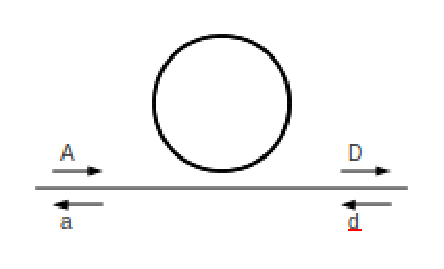
\includegraphics[width=0.49\textwidth]{anillo}              
  \includegraphics[width=0.49\textwidth]{SEM}
  \caption{Electron microscopy image of a ring resonator fabricated in our facilities. Starting from SOI wafers with 3~$\mu m$ buried oxide and 250~nm silicon layer, waveguides were patterned with e-beam lithography and etched with an inductively coupled plasma (ICP) etcher. The structures were covered with 2~$\mu m$ of silica after SEM characterization. The channels were 500~nm wide and 250~nm high, and were coupled to a 10~$\mu m$-radius ring through a 300~nm gap.
  }

\end{figure}


\subsection{Testing}
Devices were tested in fully equipped laboratories, with capacity of ultrafast nonlinear measurements. For this, the center has several laser sources (tunable, pulsed and continuous) in the range of 1.3-1.6 microns, coupling systems (fiber, objective or grating), and detection systems with bandwidths above 40~GHz. Nonlinear experiments include pump and probe measurements, where a pump generates changes in the propagation of a signal by cross-absorption-modulation (XAM) and cross-phase-modulation (XPM). These changes can be exploited for all-optical switching and logic gates (Section~\ref{ch:allOpticalSwitching}). For this, I used Mach-Zehnder interferometers or ring resonators to convert phase modulation into amplitude modulation.
Finally, I characterized the lifetime of the carriers (\ref{ch:timeRes}), which is decisive to determine the maximum switching speed of the devices and investigated parametric processes such as four wave mixing, as it has recently been shown that, under certain conditions, it can be efficient in silicon guides (\ref{ch:fwm}).


\begin{figure}[htb]
  \centering
  \includegraphics[width=0.49\textwidth]{horizontal2}            
  \includegraphics[width=0.49\textwidth]{vertical2}
  \caption{Horizontal and vertical coupling setups for sample characterization.}
\end{figure}



\section{Outline}
Chapter~\ref{ch:PhotonicCircuits} introduces the building blocks and chapter~\ref{ch:nonlinearEffects} the nonlinear effects that play a role for developing all-optical switches.
Chapters~\ref{ch:paperSwitching}-\ref{ch:paperLogicGates} present an all optical switch and a logic gate, using a microring resonator and a Mach Zehnder Interferometer respectively.
Chapters~\ref{ch:articleTimeRes}-\ref{ch:articleFigureOfMerit} characterize the figures of merit of different nonlinear waveguides.
Then, appendix~\ref{ch:experimentalSetups} describes the different experimental setups, where Ref.~\ref{ch:paperBackscattering} presents a technique to characterize rings that considers backscattering effects through a model and Ref.~\ref{ch:paperPhase} is a technique to measure the phase of different devices. Finally, appendix~\ref{ch:simulations} covers different simulation algorithms used for this dissertation.


\pagestyle{plain}
\bibliographystyle{unsrt}
\bibliography{library}


\pagestyle{fancy}
\lhead{}
\renewcommand{\chaptermark}[1]{\markboth{\thechapter.\ #1}{}}

\chapter{Building blocks}
\label{ch:PhotonicCircuits}
The most important building blocks for developing all-optical switches are:


\section{Waveguides}

To route light in photonic integrated circuits there are different types of waveguides:

\begin{figure}[h]
    \centering
    \includegraphics[width=0.49\textwidth]{strip3d2}
    \includegraphics[width=0.49\textwidth]{rib3d}
    \caption{The strip (left) confines more the light than the rib waveguide (right). However, in the strip, the mode sees more sidewall roughness created during the etching process and usually has higher loss.}
    \label{fig:ribStripSchematics}
\end{figure}


\begin{itemize}
 \item In \textbf{Strip} waveguides, the silicon is fully etched at both sides. This maximizes the lateral index contrast, allowing very tight bends and small footprints. Sidewall roughness is the main source of loss, which is usually in the range of few dB/cm for $220 \times 500$~nm waveguides.

 \item In \textbf{Rib} waveguides, a silicon slab remains at the bottom, where the mode expands. The index difference and confinement factor are smaller than the strip case, requiring higher bending radius. However they can achieve lower loss and allow the introduction of an electrical signal from both sides of the slab, as for example in modulators.
 
 \item If a thin layer of low-index material is inserted in the middle of the core of a strip waveguide, that is called a \textbf{slot} waveguide. These waveguides are interesting for some applications because the mode with polarization perpendicular to the slot layer undergoes a strong field enhancement due to the dielectric constant discontinuity. The orientation of the slot layer can be either horizontal or vertical.
 For sensing, a vertical slot is very interesting, as the slot can be filled with the analyte, whereas for nonlinear applications the horizontal slot has lower loss and therefore longer effective length of the nonlinear interaction.
\end{itemize}


\begin{figure}[h]
    \centering
    \includegraphics[width=0.49\textwidth]{sloth}
    \includegraphics[width=0.49\textwidth]{slotv}
    \caption{The slot can be filled with an analyte (sensors) or a nonlinear material (silicon nanocrystals) and can be horizontal or vertical.}
    \label{fig:slotSchematic}
\end{figure}


There are several methods to calculate the modes in a waveguide (Appendix~\ref{ch:simulations}).
All of them calculate the possible modes that can propagate inside the waveguide, together with its propagation constant and effective index.
Moreover light can travel with two different orthogonal polarization states, quasi transverse-electric (quasi-TE) and quasi transverse-magnetic (quasi-TM), that we refer as TE and TM for simplicity.


\begin{figure}[h]
    \centering
    \includegraphics[width=0.49\textwidth]{te0}
    \includegraphics[width=0.49\textwidth]{tm0}
    \caption{Fundamental transverse-electric TE (left) and magnetic TM (right) modes of a $220\times500~$nm silicon strip waveguide surrounded by silica. In both cases we plot the highest component of the electrical field, which is the horizontal component for TE (Ex) and the vertical (Ey) for TM at 1.55~$\mu$m.}
    \label{fig:modesStrip}
\end{figure}


\begin{figure}[h]
    \centering
    \includegraphics[width=0.49\textwidth]{te0rib}
    \includegraphics[width=0.49\textwidth]{tm0Slot}
    \caption{Left: Fundamental TE mode of a $220\times500~$nm silicon rib waveguide with a 100~nm silicon slab. Right: Fundamental TM mode of a slot waveguide that consists of two $220\times500~$nm silicon slabs separated by a 100~nm silica slot. We can see that the mode expands in the 120~nm slab of the rib waveguide (left) and that the 100~nm silica slot confines the mode inside the slot thanks to the field enhancement discontinuity of both silicon slabs (right). In both cases we plot the highest component of the electrical field, which is the horizontal component for TE (Ex) and the vertical (Ey) for TM at 1.55~$\mu$m}
    \label{fig:modesRibSlot}
\end{figure}


\begin{figure}[h]
    \centering
    \includegraphics[width=0.7\textwidth]{modesSilicon}
    \caption{Effective index for different modes and waveguide widths of a 220~nm height Silicon strip waveguide. The graph shows the guided modes that can propagate inside the waveguide, whose index is above the refractive index of the Silica (1.44).}
    \label{fig:modesSilicon}
\end{figure}


\section{Bends}
Bend waveguides are necessary in all photonic circuits, specially for designing ring resonators and connecting different components. It is therefore of utmost importance to understand light propagation inside the bend.
Bent modes can be calculated using standard mode solvers using a conformal transformation of the index profile as explained in~\cite{Heiblum:75}.
The bend introduces an asymmetry in the mode profile, which can be modeled with a good approximation as an index increase towards the outer side of the bend. This effect pushes the mode to the outer part of the bend, and bend loss occurs in form of radiation losses.

However, Silicon waveguides allow very small bending radius thanks to the high refractive index between the silicon core (3.47) and silica cladding (1.44), enabling high scale integration of photonic integrated circuits. In Fig.~\ref{fig:90bendLoss} we can see that for a strip waveguide with 5~$\mu$m bending radius, losses are lower than 0.04~dB per 90$^\circ$ turn.

\begin{figure}[h]
    \centering
    \includegraphics[width=1.0\textwidth]{bendModes015}
    \caption{1.55~$\mu$m TE Computed mode of a $220\times500~$nm strip waveguide with no bend (left), 5~$\mu$m (center) and 1~$\mu$m (right) bending radius, where the leaking of the mode to the cladding increases significantly.}
    \label{fig:bendLoss015}
\end{figure}


\begin{figure}[h]
    \centering
    \includegraphics[width=0.6\textwidth]{bendRadius_silicon_bp_2d_0p45_TE_2p85deltaN}
    \caption{Simulated losses of a 90$^\circ$ bend for different bending radius. As we can see, strip waveguides allow very small bending radius thanks to the high confinement of the mode inside the Silicon.}
    \label{fig:90bendLoss}
\end{figure}

\section{Fiber to chip coupling}
Coupling between integrated circuits and optical fibers is a serious challenge because of their mode size mismatch. There two main approaches to solve this problem:

\begin{itemize}
 \item Using a \textbf{grating coupler} to couple light from a fiber into the chip~\cite{1017613} allows device testing directly from the wafer. It is based on a resonant structure and must be designed for a certain polarization and wavelength range.
 
 \item We can couple light \textbf{horizontally} with a taper that adapts the mode size from the chip to the fiber. %inside the waveguide to match the mode of the fiber.
 A regular taper only expands the mode horizontally, while an inverse taper narrows the mode first and then it expands in both directions with a more uniform shape.
 Inverse tapers increase the coupling efficiency, but are more sensitive to fabrication tolerances~\cite{Shoji:02}.
 
\end{itemize}



\section{Mach Zehnder interferometer (MZI)}
It is the most basic interferometric structure.
An input beam is divided into two arms with different length or different phase shifts, so the relative phase shift between both arms changes for different wavelengths, interfering either constructive or destructively. The output field is:

\begin{equation}
	E_{out}/E_{in}=cos(\Delta \phi)
\end{equation} 

Where $\Delta \phi$ is the phase difference between both arms of the interferometer, that can be due to different arm length ($\Delta \phi = \beta \Delta L$) or different propagation constant ($\beta$) in each arm ($\Delta \phi = \Delta \beta L$).

\begin{figure}[htb]
    \centering
    \includegraphics[width=0.5\textwidth]{mzi-crop}
    \caption{Schematic MZI interferometer. We can use it as a logic gate by accessing both arms independently, as in Chapter~\ref{ch:paperLogicGates} paper.}
    \label{fig:mziSchematic}
\end{figure}


\begin{figure}[htb]
    \centering
    \includegraphics[width=1.0\textwidth]{mzi13mm350um}
      \caption{Impulse response (top) and transfer function (bottom) measurements of a 350~$\mu$m arm difference MZI (5~ps) using an Optical Vector Analyzer (OVA) (Appendix~\ref{ch:method}). From the Inverse Fourier Transform of the spectrum we can measure the delay between both arms.}
    \label{fig:mzi13mm350um}
\end{figure}


\begin{figure}[htb]
    \centering
    \includegraphics[width=0.35\textwidth,angle=-90]{mziOn} \includegraphics[width=0.35\textwidth,angle=-90]{mziOff}
      \caption{MZI interferometer with constructive (left) and destructive (right) interference.}
    \label{fig:mziOnOff}
\end{figure}



\section{Ring resonators}
Ring resonators are very useful components for filtering, multiplexing, switching and modulating.
An optical ring resonator is a structure formed connecting the input of a directional coupler to one of the outputs (Fig.~\ref{fig:ringSchematic}).
When we couple light of a certain wavelength into the ring, it generates constructive or destructive interference in the multiple turns, so only the wavelengths that satisfy the resonance condition remain inside the ring, which are multiples of the ring length.
The rest of the wavelengths accumulate different phase shifts along the ring and interfere destructively.

\begin{figure}[htb]
    \centering
    \includegraphics[width=0.5\textwidth]{ring}
    \caption{A is the single pass amplitude transmission and k/t the (cross/self)-coupling coefficient of the ring.}
    \label{fig:ringSchematic}
\end{figure}

The transmission equation of a ring can be easily obtained. If we consider an input field $E_{in}$, the first contribution at the output is $E_{in} t$ being $t$ the transmission in the coupler (Fig.~\ref{fig:ringSchematic}).
The second contribution ($-E_{in} k^2$) has the ring single pass amplitude transmission ($A=|A| e^{j\phi}$), two coupling coefficients ($k^2$) and a negative sign due to the $\pi/2$ shift to enter the ring and another $\pi/2$ phase shift to go back into the waveguide.

\begin{equation}
	E_{out}=E_{in}[t-k^2A-k^2tA^2 + \ldots]
\end{equation} 

\begin{equation}
	E_{out}/E_{in}=t-k^2A[1+tA + (tA)^2 +  \ldots]
\end{equation} 

Where the sum of the infinite terms of a geometric progression of common ratio $tA<1$ is $ S_\infty = \frac{1}{1-tA} $

\begin{equation}
	E_{out}/E_{in}=t-k^2A\frac{1}{1-tA}
\end{equation} 

\begin{equation}
	E_{out}/E_{in}=\frac{t-t^2A-K^2A}{1-tA}
\end{equation} 

And we know that $k^2+t^2=1$, so we can substitute $k^2=1-t^2$:

\begin{equation}
	E_{out}/E_{in}=\frac{t-A}{1-tA}
\label{eq:transmissionRing}
\end{equation}

Where the single pass amplitude transmission ($A=|A| e^{j\phi}$) in resonance ($\phi=\beta L=2\pi \frac{ n_{eff}}{\lambda} 2 \pi R= 0,2\pi,4\pi,\ldots$), only has the losses term ($A=\alpha$).
Depending on the relation between the coupling coefficient and the losses, a ring resonator is:

\begin{itemize}
\item \textbf{Under-coupled ($t>A$):}  The coupling is lower than the attenuation in a single trip through the ring. With zero phase at the resonances, each resonance produces a phase fluctuation. 

\item \textbf{Critically coupled ($t=A$):} The attenuation in one trip through the ring equals the coupling coefficient. In this case there is zero transmission at resonance, because the output light coming from the ring and from the input port cancel out.
 
\item \textbf{Over-coupled ($t<A$):} The coupling coefficient is higher than the attenuation through the ring. Therefore the phase accumulates an extra $2\pi$ at each resonance because at the output, more energy is coming from the ring than from the input port, generating an extra phase delay. The phase at the resonance is $\pi$.
\end{itemize}


% \begin{figure}[htb]
%     \centering
%     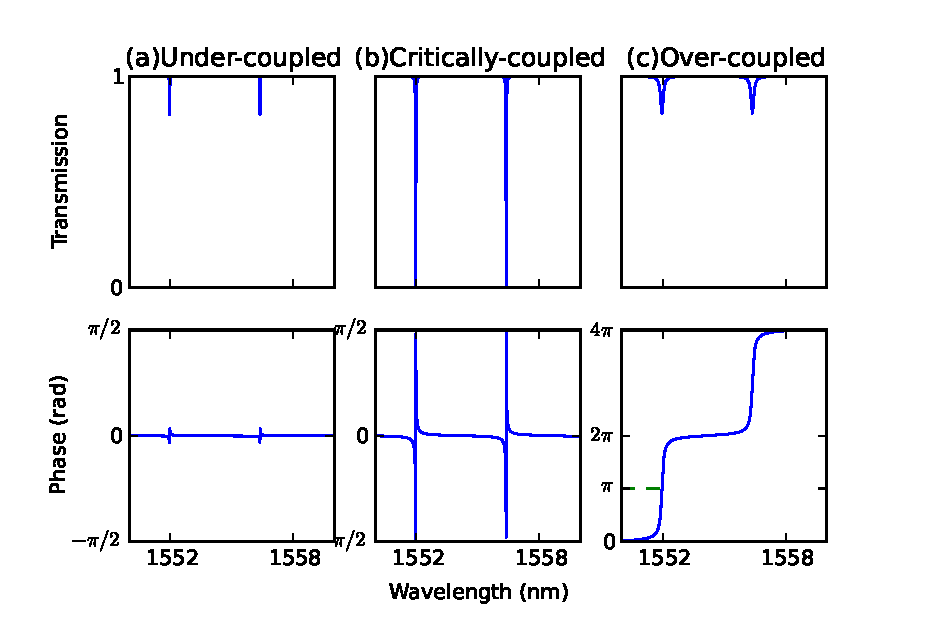
\includegraphics[width=1.0\textwidth]{ringCouplingRegimes}
%     \caption{Simulated transmission and phase spectra of a ring resonator under different coupling regimes.
%     A= 0.99 in all cases, and $t$ is 0.999, 0.99, 0.9 in the left, center and right panels respectively.
%     Distinguishing over- from under-coupling regimes requires the phase response.}
%     \label{fig:ringDifferentCouplingTesis}
% \end{figure}


Rings have a certain free spectral range (FSR), extinction ratio (ER), and resonance full-width half maximum (FWHM), related to the quality factor (Q) and finesse ($F$). These parameters depend not only on the coupling (k) and the amplitude transmission inside the ring (A), but also on manufacturing tolerances~\cite{Bogaerts:12}.

\begin{equation}
	FSR=\frac{\lambda_{res}^2}{n_gL}
\end{equation} 

Where $n_g$ is the group index and $\lambda_{res}$ is the resonant wavelength.

\begin{equation}
	Q=mF=m\frac{FSR}{FWHM}
\end{equation} 

% \begin{figure}[htb]
%     \centering
%     \includegraphics[width=1.0\textwidth]{r20g280TMP13f}
%       \caption{Impulse response (top) and transfer function (bottom) measurements of a 20~$\mu$m radius ring resonator with 280~nm gap and transverse-magnetic (TM) polarization. From the separation between the resonances (FSR) we can extract the group index ($n_g=4.33$).}
%     \label{fig:r20g280TMP13f}
% \end{figure}


$McKinnon~et~al$~\cite{McKinnon2009} develop a method for extracting the coupling and loss coefficients.
However, their formulas do not distinguish which coefficient is loss and which is coupling, so in paper~\ref{ch:paperPhase} we propose a novel experimental technique able to distinguish unambiguously the parameters of the ring. %citaPaperJSQTE
Moreover, when working with very high quality factors ($Q>10k$), backscattering effects can greatly alter the shape to the resonances, so in paper~\ref{ch:paperBackscattering} we present a theoretical model that considers backscattering effects and experimental measurements that demonstrate its validity~\cite{Ballesteros2011}.

% A ring resonator is a very interesting structure for all-optical switching.
% As we want to switch a signal using a control signal, both of them need to satisfy the resonance condition so they can enter the ring and interact in the multiple turns inside the ring.

% \subsection*{MZI as a Logic gate}
% If we access only one of the arms of the Mach Zehnder interferometer we can use it as a logic gate.
% As the data signals will be affecting only one of the branches of the interferometer we can imbalance the interferometer inducing a phase shift through cross-phase modulation (XPM).
% So if the working point is set to a minimum of the MZI, we will have signal at the output (a logic one) with only one of the branches is unbalanced, working as a exclusive OR (XOR).
% Different logic gates can also be achieved modifying the control and data ports.
% 
% 
% \begin{figure}[htb]
%     \centering
%     \includegraphics[width=0.5\textwidth]{logicGate7}
%     \caption{Schematic optical logic gate based on a MZI interferometer.
%     We can induce phase shifts in each arm through cross-absorption modulation (XPM).}%We can filter out data~1 and data~2 using ring resonators at the end of each arm (purple) or at the output.
%     \label{fig:logicGate}
% \end{figure}
% 
% \begin{table}[h]
% \centering
% \begin{tabular}{|c|c|c|} \hline
% \textbf{A} & \textbf{B} & \textbf{A XOR B}\\ \hline
% 0 & 0 & 0\\
% 0 & 1 & 1\\
% 1 & 0 & 1\\
% 1 & 1 & 0\\
% \hline
% \end{tabular}
% \caption{Truth table of a XOR logic gate.}
% \label{table:resultsImGamma}
% \end{table}



\pagestyle{plain}
\bibliographystyle{unsrt}
\bibliography{library}

\pagestyle{fancy}
\lhead{}
\renewcommand{\chaptermark}[1]{\markboth{\thechapter.\ #1}{}}

\chapter{Nonlinear effects}
\label{ch:nonlinearEffects}

There is a great scientific and technological interest in Silicon for developing photonic devices based on nonlinear processes. Table \ref{tab:nonlinearDevices} contains a selection of the most important works on the subject for the last six years.
These works can be classified according to the main nonlinear effect observed in Silicon:

\begin{itemize}
\item \textbf{Thermal effects} are the slowest (ms).
Light can heat silicon, and an increase in temperature increases its refractive index. Its coefficient is equal to $1.8 \times 10^{-4}/^\circ$C~\cite{Pruessner2007,Kiyat2006}. This effect can be beneficial in some applications where fine tuning is necessary, which can be achieved by applying temperature variations. On the other hand, this effect can be problematic when a stable performance with temperature is desired. In those cases, one can introduce a cladding material with a negative thermo-refractive coefficient in order to make the device athermal~\cite{Teng2009,Zhou2009a,Han2007}.

\item \textbf{Free carrier effects} \cite{Almeida2004,Boyraz2004,Preble2005,Liang:05,Foster2007,Waldow2008} appear at relatively high powers ($>$100~mW for the geometries presented in the thesis) and are generated through two-photon absorption (TPA). They produce changes both in refractive index (free-carrier-dispersion, FCD) ($\Delta n < 0$) and absorption (free-carrier absorption, FCA) that can be used for switching one beam using another co-propagating beam. The problem is that the carriers take nano-seconds to recombine, limiting the switching to around 1~GHz speed.


\item \textbf{Kerr effect} \cite{Hochberg2006,Martinez2010} is produced by the third order nonlinear coefficient $\chi^{(3)}$, and has the advantage of having instantaneous response time, which introduces no speed limitations.
The problem is that the power levels needed also create carriers through TPA, and these carriers hinder the Kerr effect.
One strategy to increase the Kerr response is to include materials with a high $\chi^{(3)}$ in the waveguide section. Another possibility is to use amorphous silicon, which has a lower TPA coefficient and very fast carrier recombination time~\cite{Matres2013}.

\item \textbf{Pockels effect} is produced by the second order nonlinear coefficient, $\chi^{(2)}$. The problem is that it appears only in materials with no inversion center, such as $\mathrm{LiNbO}_3$, and in silicon, is zero. However, depositing a $\mathrm{Si_3N_4}$ layer, one can induce stress and break the symmetry of Silicon~\cite{Jacobsen2006,Cazzanelli2012,Chmielak2011}.
\end{itemize}

\begin{table}
\centering
\begin{tabulary}{1.00\textwidth}{|L|L|L|L|L|}\hline 
\textbf{Ref.} & \textbf{Group} & \textbf{Structure} & \textbf{Effect} & \textbf{Details}\\ \hline
\cite{Almeida2004b} & Cornell & Ring & carriers (FC) generated through TPA & 450~ps response\\ \hline
\cite{Boyraz2004} & UCLA & Mach-Zehnder & Kerr + FC & 7~ns response due to carriers\\ \hline
\cite{Preble2005}& Cornell & Ring & FC generated through TPA & 7~ns response due to carriers\\ \hline
\cite{Liang:05}& IMEC - Ghent  & Waveguide & XAM & 13~ps response, 2~W peak power\\ \hline
\cite{Hochberg2006}& Caltech  & Si+ polymer & kerr & 1~ps response, 50~mW peak power but only 0.3dB modulation\\ \hline
\cite{Jacobsen2006} & Tech. Univ. of Denmark  & Si with strain & $\chi^{(2)}$ induced through strain &  measurement $\chi^{(2)} =15~$pm/V \\ \hline
\cite{Foster2007} & Cornell  & Ring & FC generated by TPA & 1~ns response, 30~mW peak power 	\\ \hline
\cite{Waldow2008} & Aachen Univ.  & Ring & fast carriers thanks to O implantation & 25~ps response with non-guided pump (800~nm) 	\\ \hline
\cite{Lee2009} & Cornell  & Waveguide & FWM & 40~Gbps conversion, 15~dB efficiency 	\\ \hline
\cite{Koos2009} & Kalsruhe Univ., IMEC  & Si slot with polymer & FWM & 3~ps response	\\ \hline
\cite{Martinez2010}& Univ. Politec. Valencia & Ring (slot waveguide with Si-nanocrystals)  & kerr & 10~ps response 	\\ \hline
\end{tabulary}
\caption{Recent impact contributions in the area of nonlinear silicon photonics.}
\label{tab:nonlinearDevices}
\end{table}



\section{Kerr effect}
% Kerr effect is produced by the third order nonlinear $\chi^3$ coefficient and is the most desired due to its high speed ($10^{-15}~\mathrm{s}$).
% Kerr effect is produced by the third order nonlinear $\chi^3$ coefficient, that has a quadratic dependence on the electric field ($\Delta n = \lambda K E^2$ ), where $\lambda$ is the wavelength of the light, K is the Kerr constant, and E is the strength of the electric field

Kerr effect produces a refractive index change ($\Delta n = n_2 I$) that depends on the optical intensity (I) and nonlinear refractive index ($n_2$). For silica, $n_2$ is typically in the order of $2.7\times10^{-16} \mathrm{cm^2/W}$ , whereas in Silicon, it is significantly higher ($4.5\times10^{-14} \mathrm{cm^2/W}$) \cite{Dinu2003a}.
Moreover, the strong confinement of the mode in small waveguides, enhances nonlinear effects, so it is more convenient to use the nonlinear coefficient ($\gamma$) definition:

\begin{equation}
 Re(\gamma) = \frac{n_2\omega}{cA_{eff}}
\label{eq:gamma}
\end{equation}

where the effective area ($A_{eff}$) is defined as in paper~\cite{Rukhlenko2012}:

\begin{equation} 
  A_{eff}= \frac{(\iint |E(x,y)|^2 dxdy)^2}{\iint |E(x,y)|^4 dxdy}
\label{eq:aeff}
\end{equation}


Kerr effect is the most desired due to its high speed ($10^{-15}~\mathrm{s}$).
However it is a very weak effect that requires power densities higher than Free carrier generation, so it is masked by the effects of these carriers.
It can be maximized with structures that confine the power in a small area, such as slot waveguides~\cite{Martinez2010}, or combining silicon with other materials with a higher $\chi^3$ coefficient, such as silicon nano-crystals~\cite{Spano2009} or some polymers~\cite{Koos2009}.
Since the Kerr constant of silicon is positive it produces an increase in refractive index ($\Delta n > 0$) and is responsible for the nonlinear optical effects of Four Wave Mixing (FWM), Self-phase modulation (SPM) and Cross-phase modulation (XPM).

\begin{itemize}
\item \textbf{Four Wave Mixing (FWM)} is a nonlinear effect in which using two wavelengths, two other are generated on both sides of the spectrum.
It is a phase-sensitive process, so the interaction depends on the relative phases between both signals and can accumulate over long distances when they satisfy a phase-matching condition, which depends on the wavelength separation and the even dispersion coefficients ($\beta_2$, $\beta_4$ , etc.).
In other cases, where there is a strong phase mismatch, four-wave mixing is not efficiently generated.
Moreover, free carrier generation also limits its efficiency.
There are several applications of FWM, such as generation of new frequencies~\cite{Bayvel1989}, wavelength conversion~\cite{Inoue1992,Lee2009} and parametric amplification \cite{Carman1966,Stolen1982,Foster2006}.

\begin{figure}[htb]
    \centering
    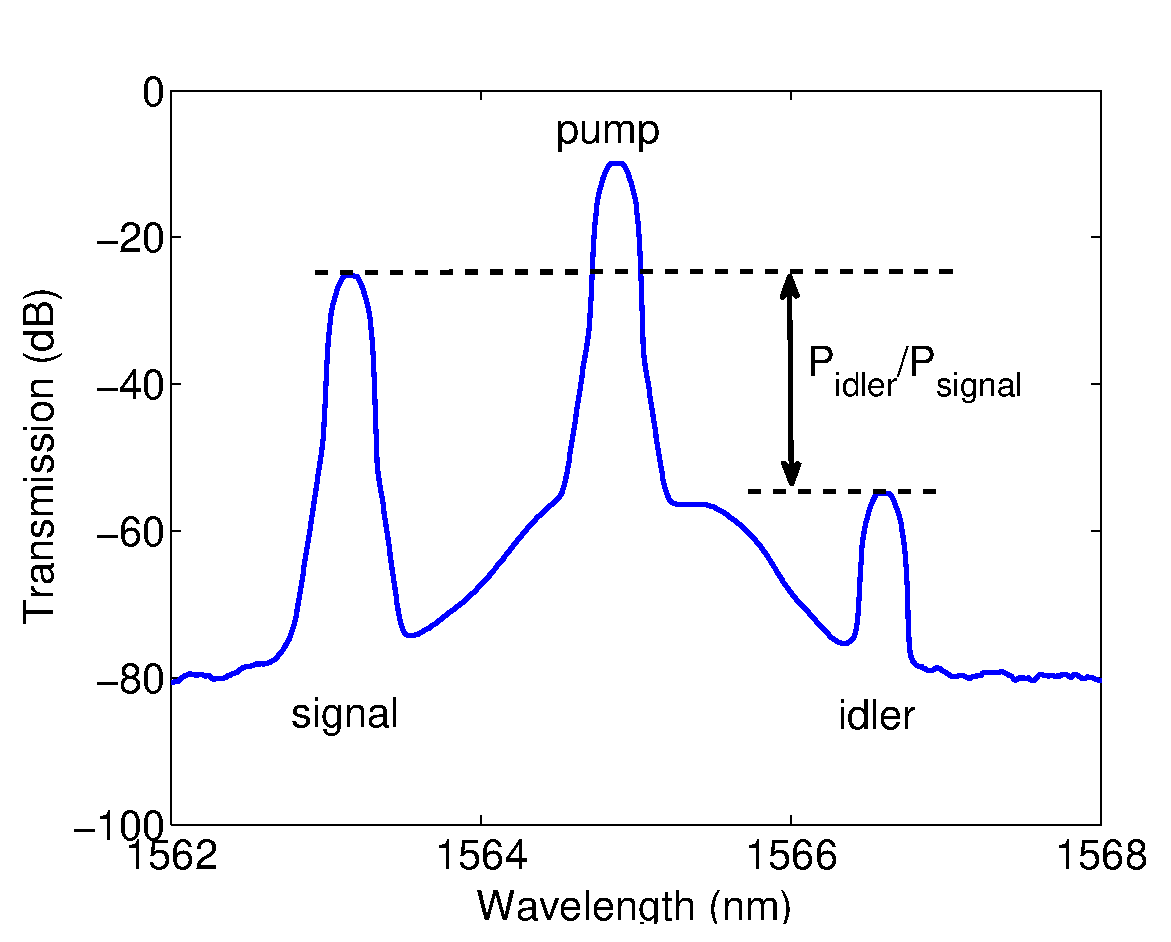
\includegraphics[width=\fWidth\textwidth]{Power_dBm_fwm_convEffMax_29p5dB}
    \caption{Generation of new frequency components via four-wave mixing.}
    \label{fig:fwmMaxEfficiency}
\end{figure}

\item \textbf{Self-phase modulation (SPM)} takes place when a short pulse of light travels in a material and induces a refractive index change during its propagation due to kerr effect. This induced chirp broadens the spectrum of the pulse as it travels. One application of SPM is the generation of super-continuum using ultrashort high peak power pulses and a nonlinear media~\cite{Boyraz2004}.

\item \textbf{Cross-phase modulation (XPM)} is a more interesting effect in terms of switching. We can use one signal to induce a refractive index change in a waveguide where another signal is traveling. Through those changes we can control one beam using another beam, changing, for example, the phase relationship between the arms of a Mach Zehnder Interferometer or the phase of a beam traveling inside a ring resonator.

\end{itemize}



\section{Two photon absorption (TPA)}
For all-optical switching, the desirable Kerr effect is limited by Two photon absorption (TPA), due to the absorption of two photons whose energy is transfered to excite an electro-hole pair.
In a waveguide, we can consider it as the imaginary part of the gamma coefficient:

\begin{equation}
 \frac{dP}{dz} = -\alpha P(z) - 2|Im(\gamma)| P(z)^2 
\label{eq:differentialTPAImGamma}
\end{equation}

where $\alpha$ and $Im(\gamma)$ are the linear and nonlinear loss and P is the power of the signal through the waveguide.

The Figure of Merit (FOM) measures the ratio between the nonlinear coefficient $Re\{\gamma\}$ and nonlinear absorption $Im\{\gamma\}$, and must be larger than two for efficient all-optical switching~\cite{Vallaitis2009,Delong1989,Mizrahi}.
We measure $Re\{\gamma\}$ through four wave mixing (appendix~\ref{ch:fwm}) and $Im\{\gamma\}$ from the nonlinear loss measurements (\ref{ch:imGamma}).
\textit{Vallaitis et al} present a way to determine a Figure of Merit which is valid without having to estimate any peak power, effective area, waveguide effective length or absorption coefficient. It only uses the nonlinear phase shift ($\Delta\phi_{NL}$) and the amplitude transmission ($T_A$) from the nonlinear time resolved measurements (\ref{ch:timeRes}):


\begin{equation} 
FOM_{TPA}=\frac{-1}{4\pi} \frac{Re\{\gamma\}}{Im\{\gamma\}} = -\frac{\Delta\phi_{NL}}{4\pi lnT_A}
\label{eq:fom}
\end{equation}

% We have mentioned several nonlinear behaviors with different characteristics. Some are desirable ($Re\{\gamma\}$) but others are not ($Im\{\gamma\}$). We must then define a way to determine the quality of the nonlinear behavior in each sample given by the Figure of Merit (FOM). Equation 1, developed in paper [2], presents a way to determine a Figure of Merit which is valid without having to estimate any peak power, effective area, waveguide effective length and absorption coefficient.

\section{Free carrier effects}
Free carriers are generated in the silicon by Two photon absorption (TPA).
We can basically differentiate two different carrier effects, all of which originate from the same TPA phenomena:

\begin{itemize}
\item \textbf{Free carrier dispersion (FCD)} produced by the refractive index change of the carriers. 

\item \textbf{Free carrier absorption (FCA)} because the excess of carriers absorb light. 
However, using a reverse polarized junction~\cite{Turner-Foster2010} or implanting dopants~\cite{Liu2006}, one can reduce the carrier lifetime and the effect of FCA.
\end{itemize}

At 1550~nm we can use the empirical formulas of free carriers, where $n_f$ is the free-carrier index (FCI) and $\alpha_f$, expressed in $cm^{-1}$, governs the free carrier absorption (FCA)~\cite{Lin2007,Soref1987}:

% \begin{equation} 
% \chi = 2n_0[n+jc\alpha/(2\omega)]
% \label{eq:chi}
% \end{equation}

\begin{equation} 
n_f = -(8.8\times 10^{-4}N_e+8.5N_h^{0.8})\times 10^{-18}
\label{eq:fcd}
\end{equation}

\begin{equation} 
\alpha_f = 1.45\times 10^{-17} N
\label{eq:fca}
\end{equation}

Carrier densities of holes ($N_h$) and electrons ($N_e$) generated through TPA are equal ($N_h=N_e=N$) and have $cm^{-3}$ units.
The negative sign in $n_f$ means a refractive index decrease due to free-carrier dispersion ($\Delta n<0$).


%Where carrier densities of holes ($N_h$) and electrons ($N_e$) are generated with equal densities through TPA ($N_h=N_e=N$) and have units of $cm^{-3}$.
%The negative sign in $n_f$ means a refractive index decrease due to free-carrier dispersion ($\Delta n<0$).

% In silicon at 1550~nm, a carrier density (N) produces free-carrier dispersion ($n_f = -5.3\times 10^{-21} N$) and absorption ($\alpha_f = 1.45\times 10^{-17} N$
%Where the carrier densities of holes ($N_h$) and electrons ($N_e$)  and are both generated with equal densities through TPA ($N_h=N_e=N$).
% \begin{equation} 
% FCI = -5.3\times 10^{-21} N
% \label{eq:fcd}
% \end{equation}
% 

% 
% Where N is the carrier density.

For all-optical switching, carriers can be the problem or the solution, according to the strategy employed.
If one managed to reduce the recombination time of carriers from 1~ns to tens of ps, the effect would be ideal for switching.
In samples fabricated through ePIXfab platform, this time was around 10~ns, while we also reported Silicon strip waveguides with recombination times in the order of 100~ps fabricated in our facilities~\cite{Oton,optoel}.
The recombination time of free carriers depends on several factors, such as dopant concentration or waveguide geometry.
Implanting dopants, such as Helium~\cite{Liu2006}, or using rib waveguides~\cite{Dimitropoulos2005} can increase the carrier diffusion and reduce carrier lifetime.
Another possibility is sweeping carriers with a p-i-n union inversely polarized, which considerably complicates the fabrication and increases the power consumption~\cite{Turner-Foster2010}.
Finally, slot \cite{Matres:12} and amorphous silicon waveguides~\cite{Matres2013} have demonstrated to reduce carrier associated effects.


\pagestyle{plain}
\bibliographystyle{unsrt}
\bibliography{library}

	

\chapter{Paper:~Ultrafast nonlinear dynamics in silicon waveguides}
\label{ch:paperSwitching}

In this work we demonstrated all-optical switching using Silicon microring resonators. 
This was possible due to the fast recombination times of the free-carriers generated during the switching.
Together with the switching experiment, we characterized the carrier lifetime using  phase sensitive ultrafast time resolved measurements.
My personal contribution to the work is the following: I did the experimental measurements, together with C. Oton; I analyzed the data and drafted the paper.
The work was presented in the 7th Optoelectronics National Meeting, and the reference is the following:


% The generated carriers had very short recombination times in comparison with other silicon waveguides.
% a 150~ps response all-optical switch with 10~dB extinction ratio based on a silicon ring resonator.
% The generated carriers had very short recombination times in comparison with other silicon waveguides.
% I this work we presented a 150~ps response all-optical switch with 10~dB extinction ratio based on a silicon ring resonator.

\vspace{1.5cm}
J. Matres, A. Martinez, J. Marti, and C. J. Oton, “Ultrafast nonlinear dynamics in silicon waveguides,” in Optoelectronics National Meeting ,7th OPTOEL, 2011, pp. 1–4.


\newpage
\begin{center}
\section*{Ultrafast nonlinear dynamics in silicon waveguides}
{J. Matres$^*$, A. Martinez, J. Marti, and C. J. Oton} 
\end{center}

\noindent
\textit{Nanophotonics Technology Center, Universidad Polit\'ecnica de Valencia, Camino de Vera s/n, 46022, Valencia, Spain}

\begin{center}
{$^*$joamatab@ntc.upv.es}
\end{center}


\textbf{Abstract} \\
\noindent
We present the ultrafast nonlinear characterization of a CMOS-compatible silicon waveguide. A phase sensitive pump and probe technique was implemented in order to monitor the phase and amplitude response of the system with 1 picosecond resolution. This allowed the characterization of carrier generation and recombination dynamics, where decay times below 150~ps were observed. With this device, we show an all-optical modulator based on an integrated microring resonator with 10~dB extinction and 1/e recovery time of 150~ps.


\section{Introduction}
Integrated silicon-based optical devices have recently emerged as a feasible technology to route, switch and modulate signals in optical networks, which are expected to dramatically reduce device costs and provide new functionalities \cite{Soref2006}. However the main limitation in these devices is that ultrafast effects, such as Kerr, require so high powers that free-carriers are generated through two-photon absorption (TPA), limiting the speed of commutators \cite{Oton}, logic gates \cite{Oton2010}, etc.
To solve this limitation there are several techniques to sweep this carriers, the most common  of them is to create a reverse biased PN junction \cite{Turner-Foster2010}.
In this work we present two different nonlinear experiments to characterize the dynamics of nonlinear effects such as Kerr, cross absorption modulation and free-carrier dispersion. In the first experiment we will observe the phase and amplitude response of high power pulses (pump) over low power pulses (probe). The other experiment is optical switching; it is also based on controlling a low-power signal (probe), through high power pulses (pump).


 
\section{Fabrication}
The samples used were fabricated from SOI wafers with 3~$\mu m$ buried oxide and 250~nm silicon layer. The waveguides were patterned with e-beam lithography and etched with an inductively coupled plasma (ICP) etcher. The structures were covered with 2~$\mu m$ of silica after SEM characterization. The channels were 500~nm wide and 250~nm high, and were coupled to a 20~$\mu m$-radius ring through a 300~nm gap. Light was coupled into the waveguides by butt-coupling with lensed fibers, and was extracted with an objective. The TM transmission spectrum was measured by tuning the laser, and the result is shown in Fig.~\ref{fig:fit20um300nmBig}, where one resonance is shown. The response was fitted to the theoretical equation~\cite{heebner2007optical} by using the propagation loss and coupling coefficient as parameters. A good agreement was found for propagation loss of 20~dB/cm and coupling coefficient k = 0.072. Full width at half depth (FWHD) of the peak was 92~pm, which corresponds to a Q-factor of 16870. 


\begin{figure}[htb]
    \centering
    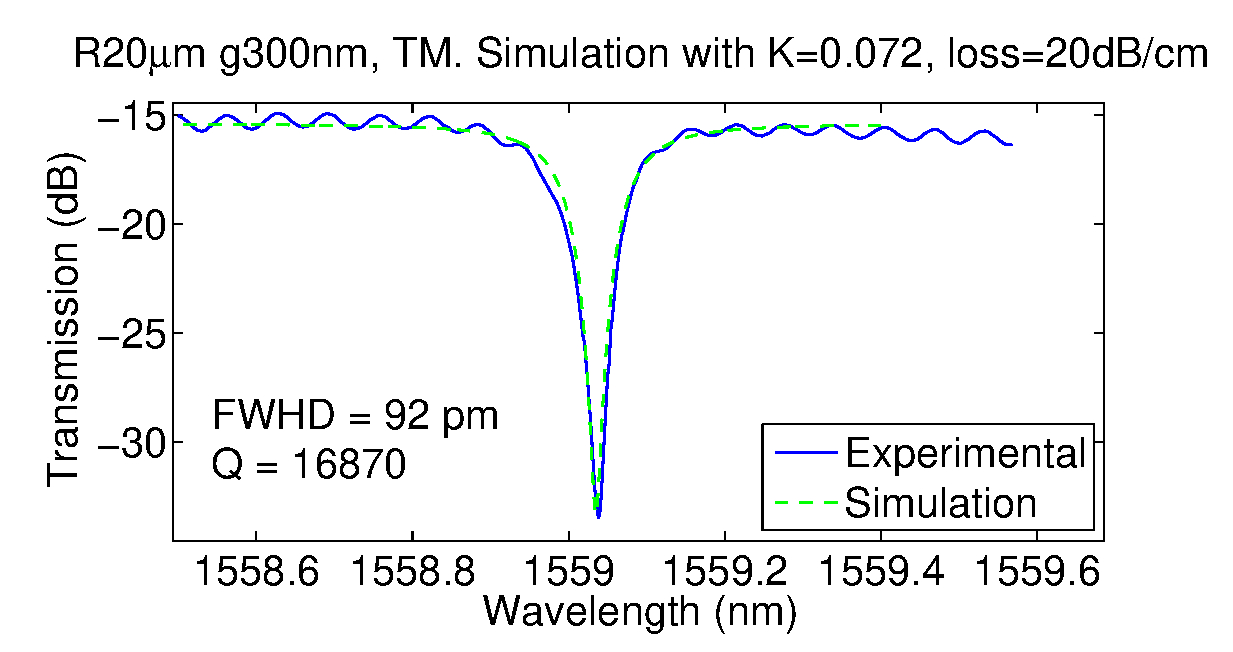
\includegraphics[width=0.8\textwidth]{fit20um300nmBig_2}   
    \caption{Transmission spectrum of the ring resonator sample (TM polarization). Solid line is the experimental data and dashed line is the result of the simulation when setting propagation loss to 20~dB/cm and coupling coefficient k = 0.072}
    \label{fig:fit20um300nmBig}
\end{figure}


\section{Experiments}

\subsection{Heterodyne characterization}
In order to study with great detail the nonlinear effects response, both in phase and module, we used an heterodyne characterization setup. The set up (Fig.~\ref{fig:timeResSetupSwitching}) consists of a series of probe pulses that are affected by a high power pulses (pump). Varying the pump pulses with respect to the probe ones we can see the module and phase response of nonlinear effects such as Kerr, cross absorption modulation and Free-carrier dispersion.


\begin{figure}[htb]
    \centering
    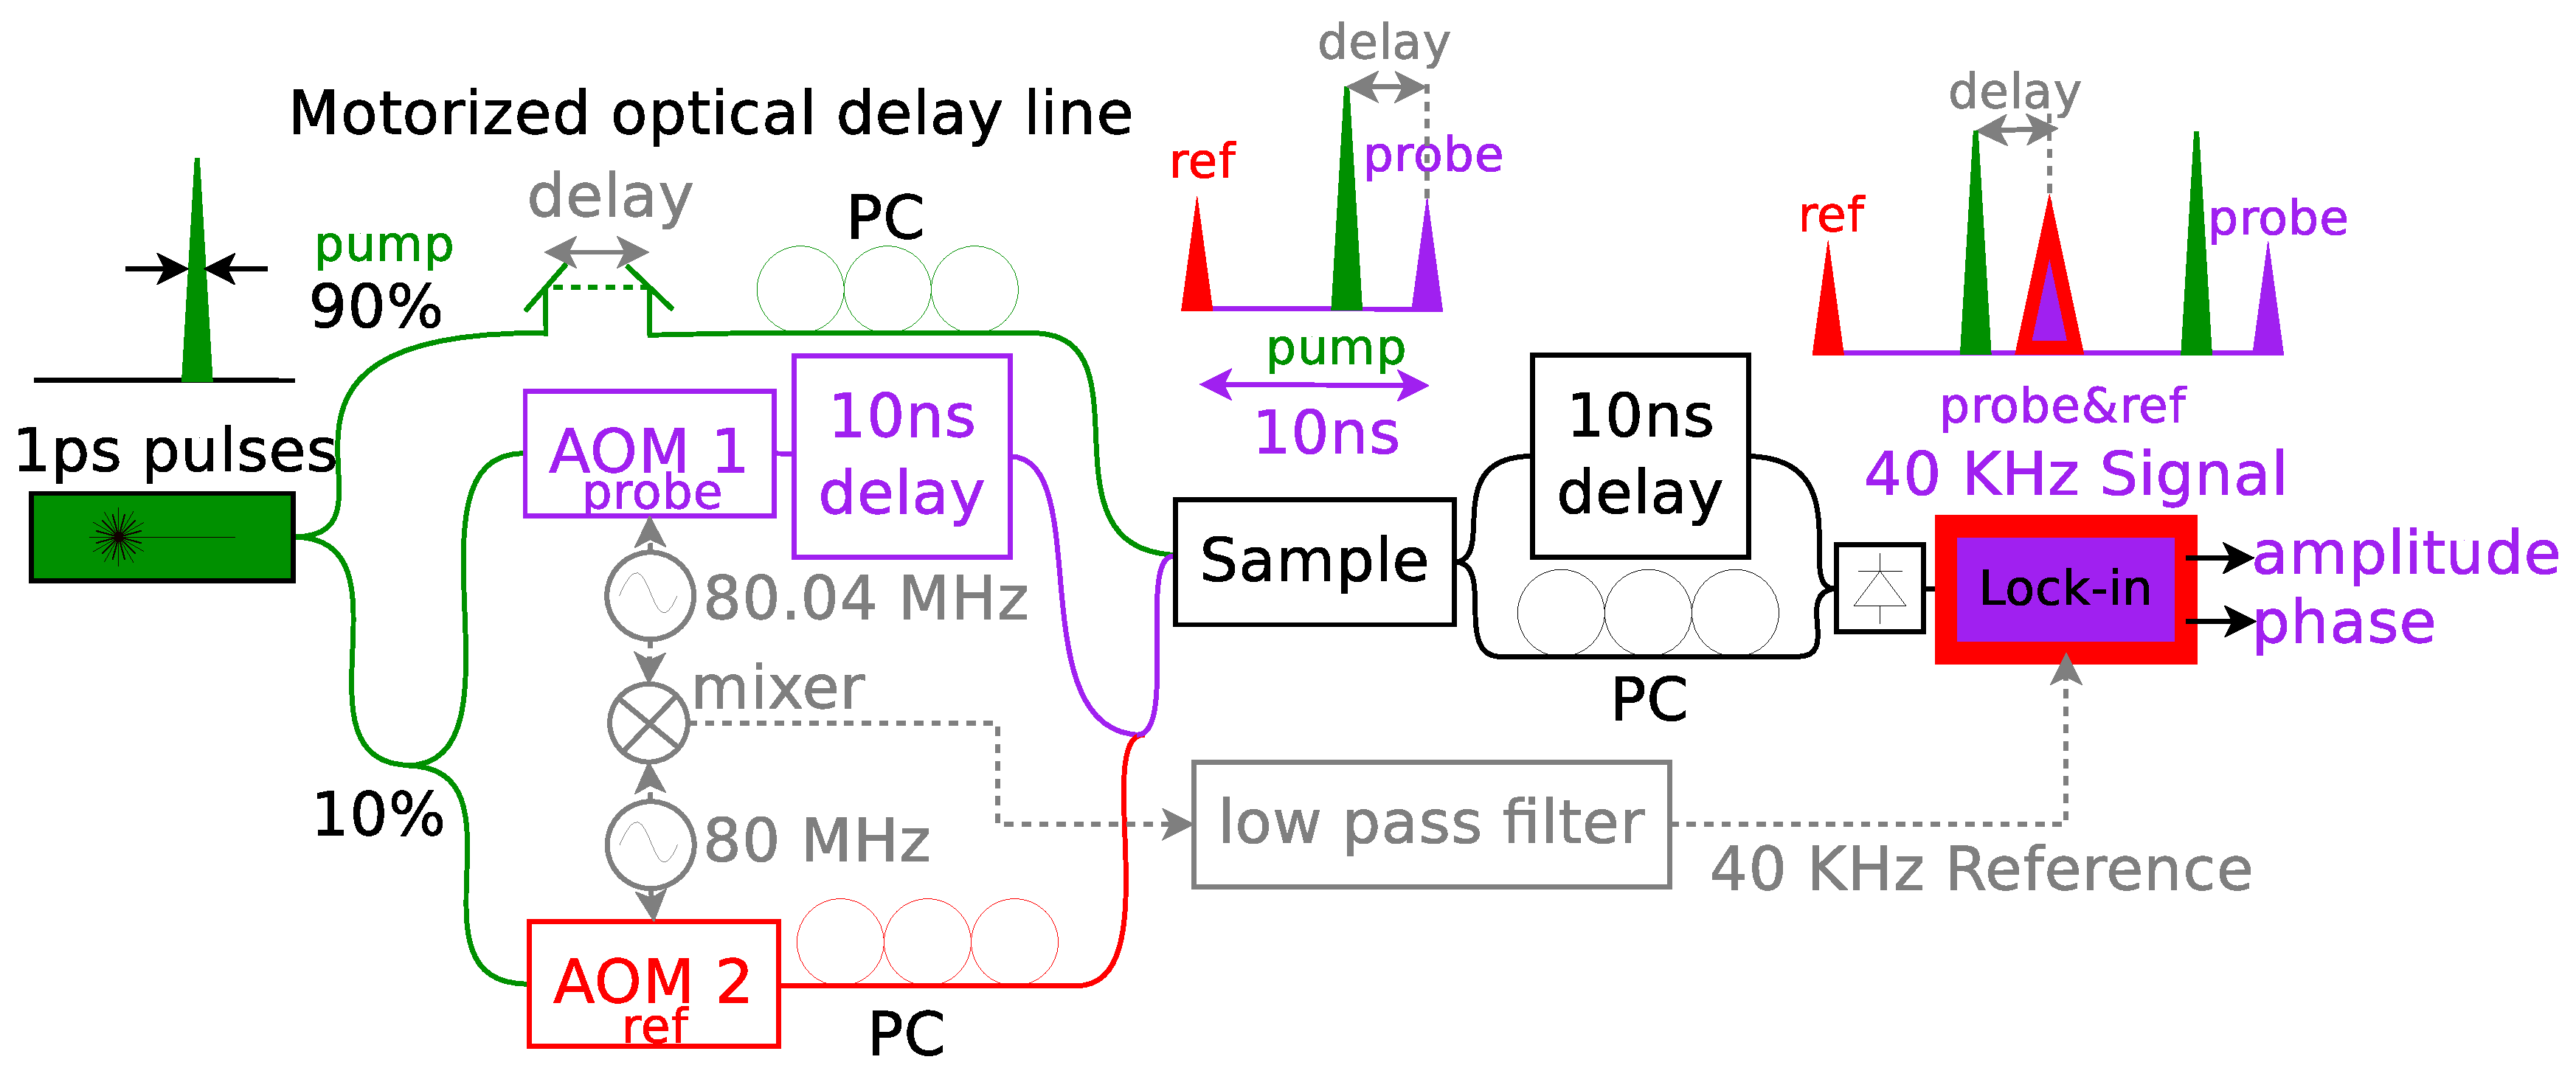
\includegraphics[width=1.0\textwidth]{timeResolvedBig}
    \caption{Characterization setup. Grey dashed line: RF signals, continuous line: optical signals. The motorized delay line was used to modify the position of the pump pulses respect the probe ones. PC: polarization controller, AOM: acousto-optic modulator.}
    \label{fig:timeResSetupSwitching}
\end{figure}


The initial pulse is divided into three pulses: two weak ones (a reference and probe separated 10~ns), and one pump pulse, situated close to the probe pulse, and whose temporal position with respect to the probe can be varied. The reference and probe pulses are recombined after passing through the sample, and the beatings they produce are collected in the lock-in. The 40~KHz beatings  are produced because the wavelengths of probe and reference signals are slightly different, as both are shifted with acousto-optic modulators which work at frequencies that only differ by 40~kHz. The amplitude and the phase of the signals are simultaneously monitored.
The amplitude collected is proportional to the amplitude of the probe pulse with respect to the reference, and the phase of the beatings corresponds to the phase shift produced by the pump to the probe pulse, considering the reference pulse as unaffected by the pump, and thus using it as a reference for the phase measurement. 


\subsection{All-optical switching}
The setup for the all-optical switching experiment is shown in Fig.~\ref{fig:switchingSetupSwitching}. A tunable laser was modulated with a $ \mathrm{LiNbO_3} $ modulator and amplified through Er-doped fiber amplifiers (EDFAs). The pulse train was generated with a 40~Gb/s bit pattern generator, where pulses had 45~ps duration and 6.4~ns period. The peak power coupled into the waveguide was estimated to be 85~mW. A continuous-wave (cw) probe signal was mixed with the pump with a 3~dB coupler and sent to the waveguide through the same fiber with an estimated coupled power of 0.5~mW. Wavelengths of pump and probe signals were respectively 1564 and 1554~nm, chosen to match with two resonances of the micro-ring resonator. The output signal was filtered to remove the pump component and amplified before sending the signal to a 50~GHz photodiode and collecting the data with a 40~GHz sampling scope.


\begin{figure}[htb]
    \centering
    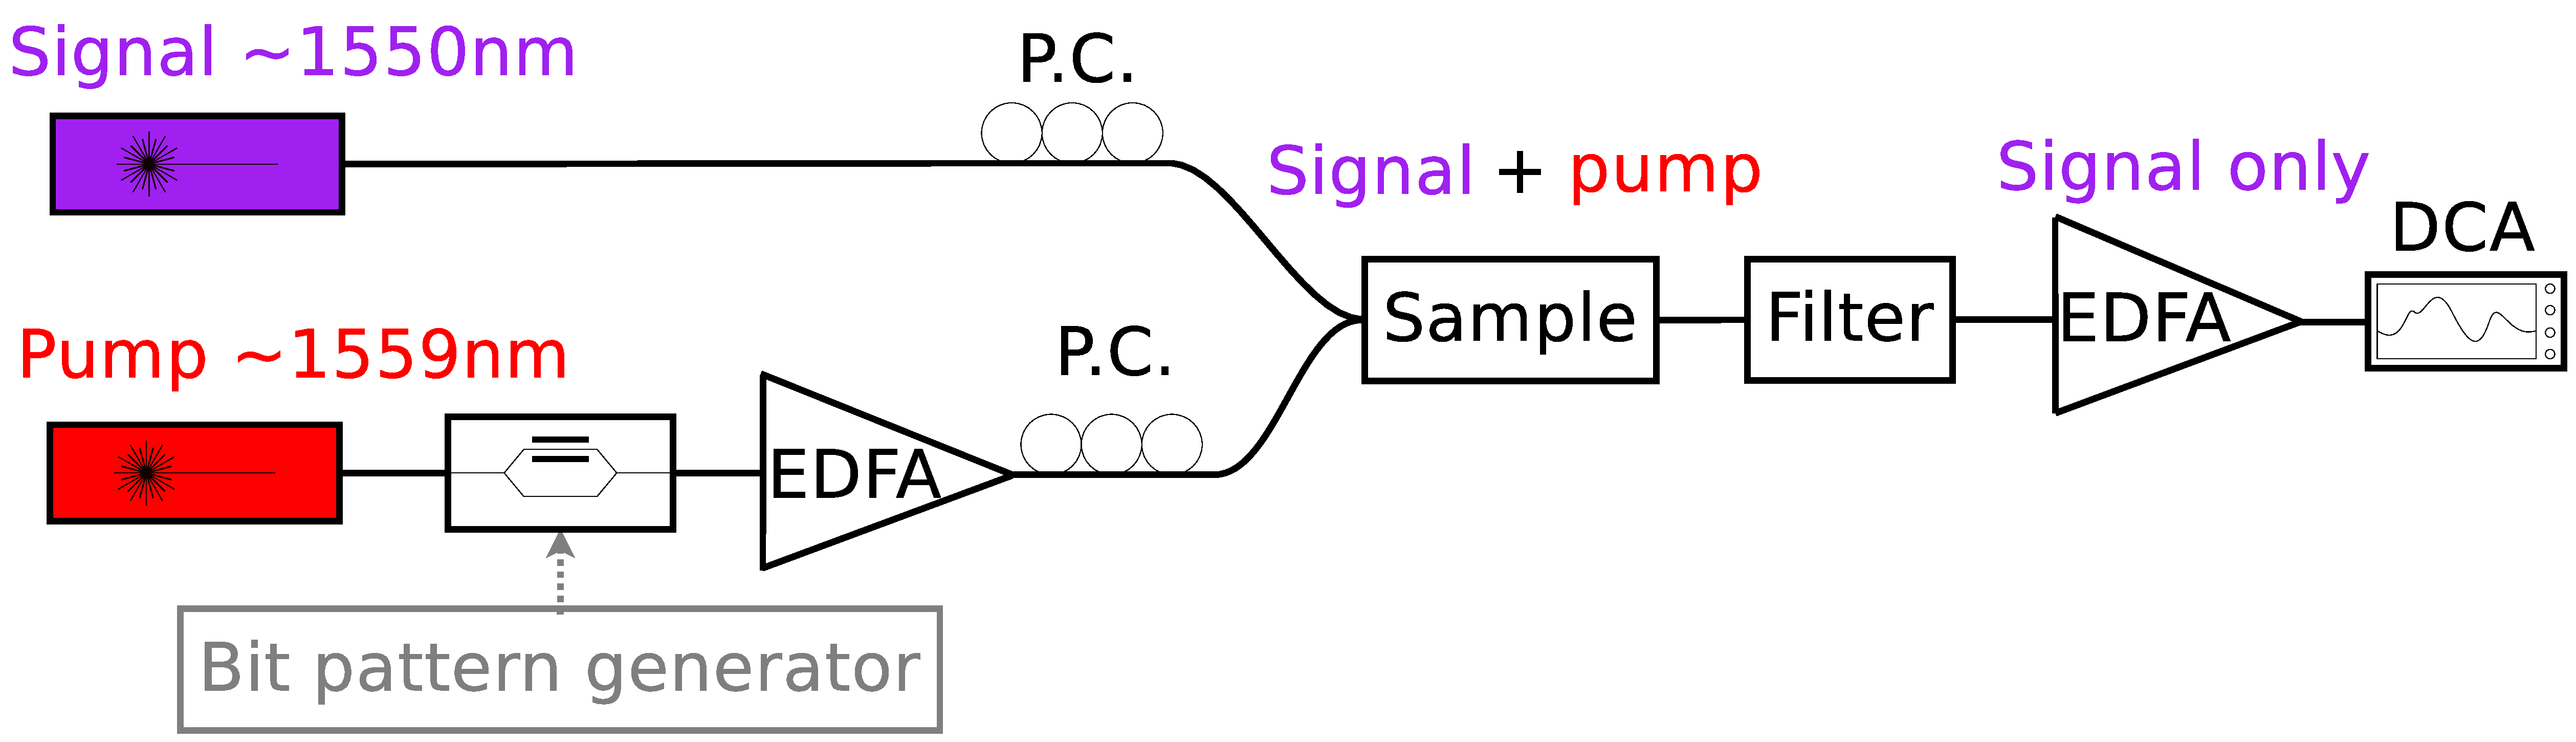
\includegraphics[width=1.0\textwidth]{switching}
    \caption{All-optical switching characterization setup. (Triangles represent EDFAs with ASE filters, PC: polarization controllers, DCA: Digital communication analyzer)}
    \label{fig:switchingSetupSwitching}
\end{figure}

\begin{figure}[htb]
    \centering
    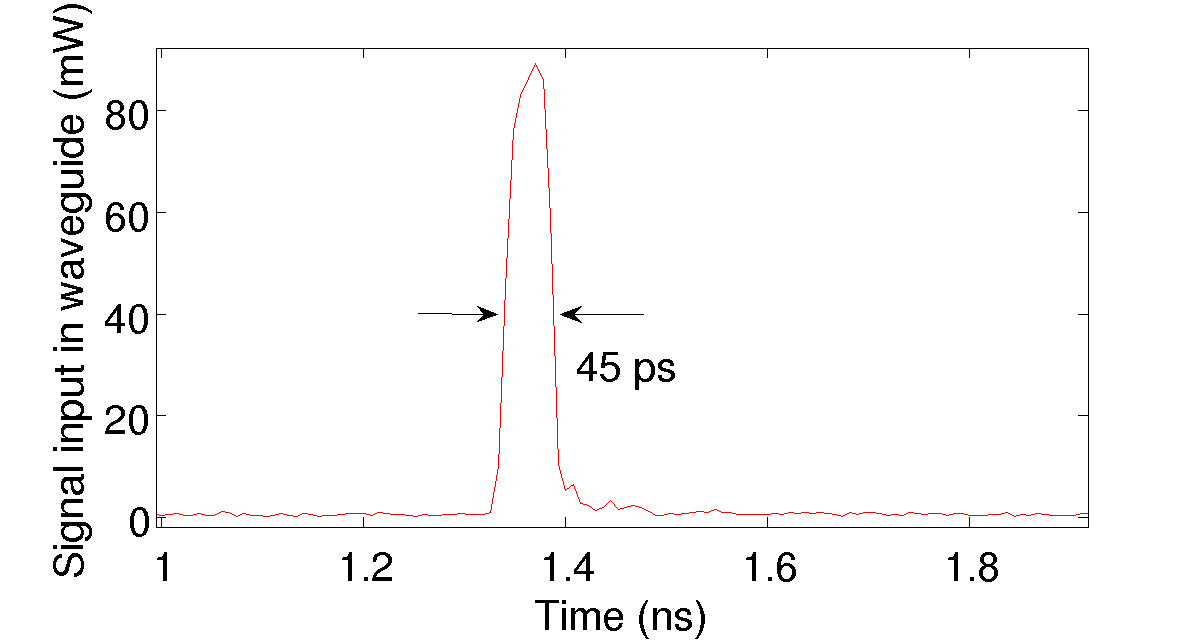
\includegraphics[width=\fWidth\textwidth]{inputPulsesSwitchingBig}
    \caption{Input pulses with 45~ps duration, 6.4~ns period and 85~mW peak power coupled in the waveguide}
    \label{fig:inputPulsesSwitchingBig}
\end{figure}

\begin{figure}[htb]
    \centering
    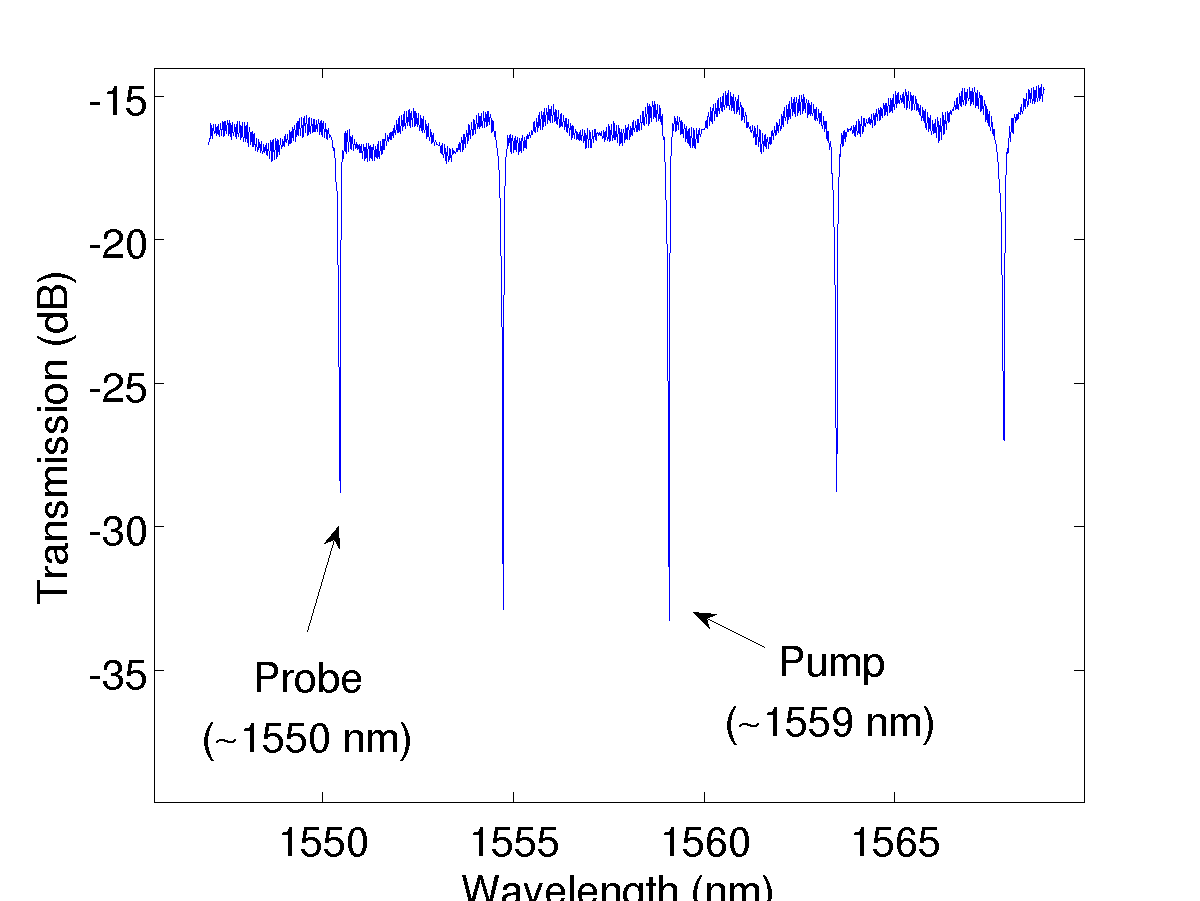
\includegraphics[width=\fWidth\textwidth]{broadBig}
    \caption{Transmission spectrum of the ring resonator sample (TM polarization). Wavelengths of pump and probe signals were respectively 1564 and 1554~nm.}
    \label{fig:transmissionSwitching}
\end{figure}

\section{Results}
\subsection{Heterodyne experiment}
In Fig.~\ref{fig:ntc02TimeResSwitching} we can see observe both Kerr and carriers effect. They produce opposite phase shifts because Kerr produces an increase in refractive index ($\Delta n > 0$) and carriers decrease it ($\Delta n < 0$).


The dynamics of each of these processes is also very different. During the pump pulse, we can see an instantaneous phase change due to Kerr effect, together with an amplitude decrease. This decrease is due to cross-absorption modulation (XAM), which consists of a two-photon absorption (TPA) process where one of the photons comes from the pump and the other comes from the probe. Once the pump pulse is gone, there is a phase response with opposite sign that remains for more than 100~ps. This is due to the carrier plasma effect, also known as free-carrier dispersion (FCD).

\begin{figure}[htb]
    \centering
    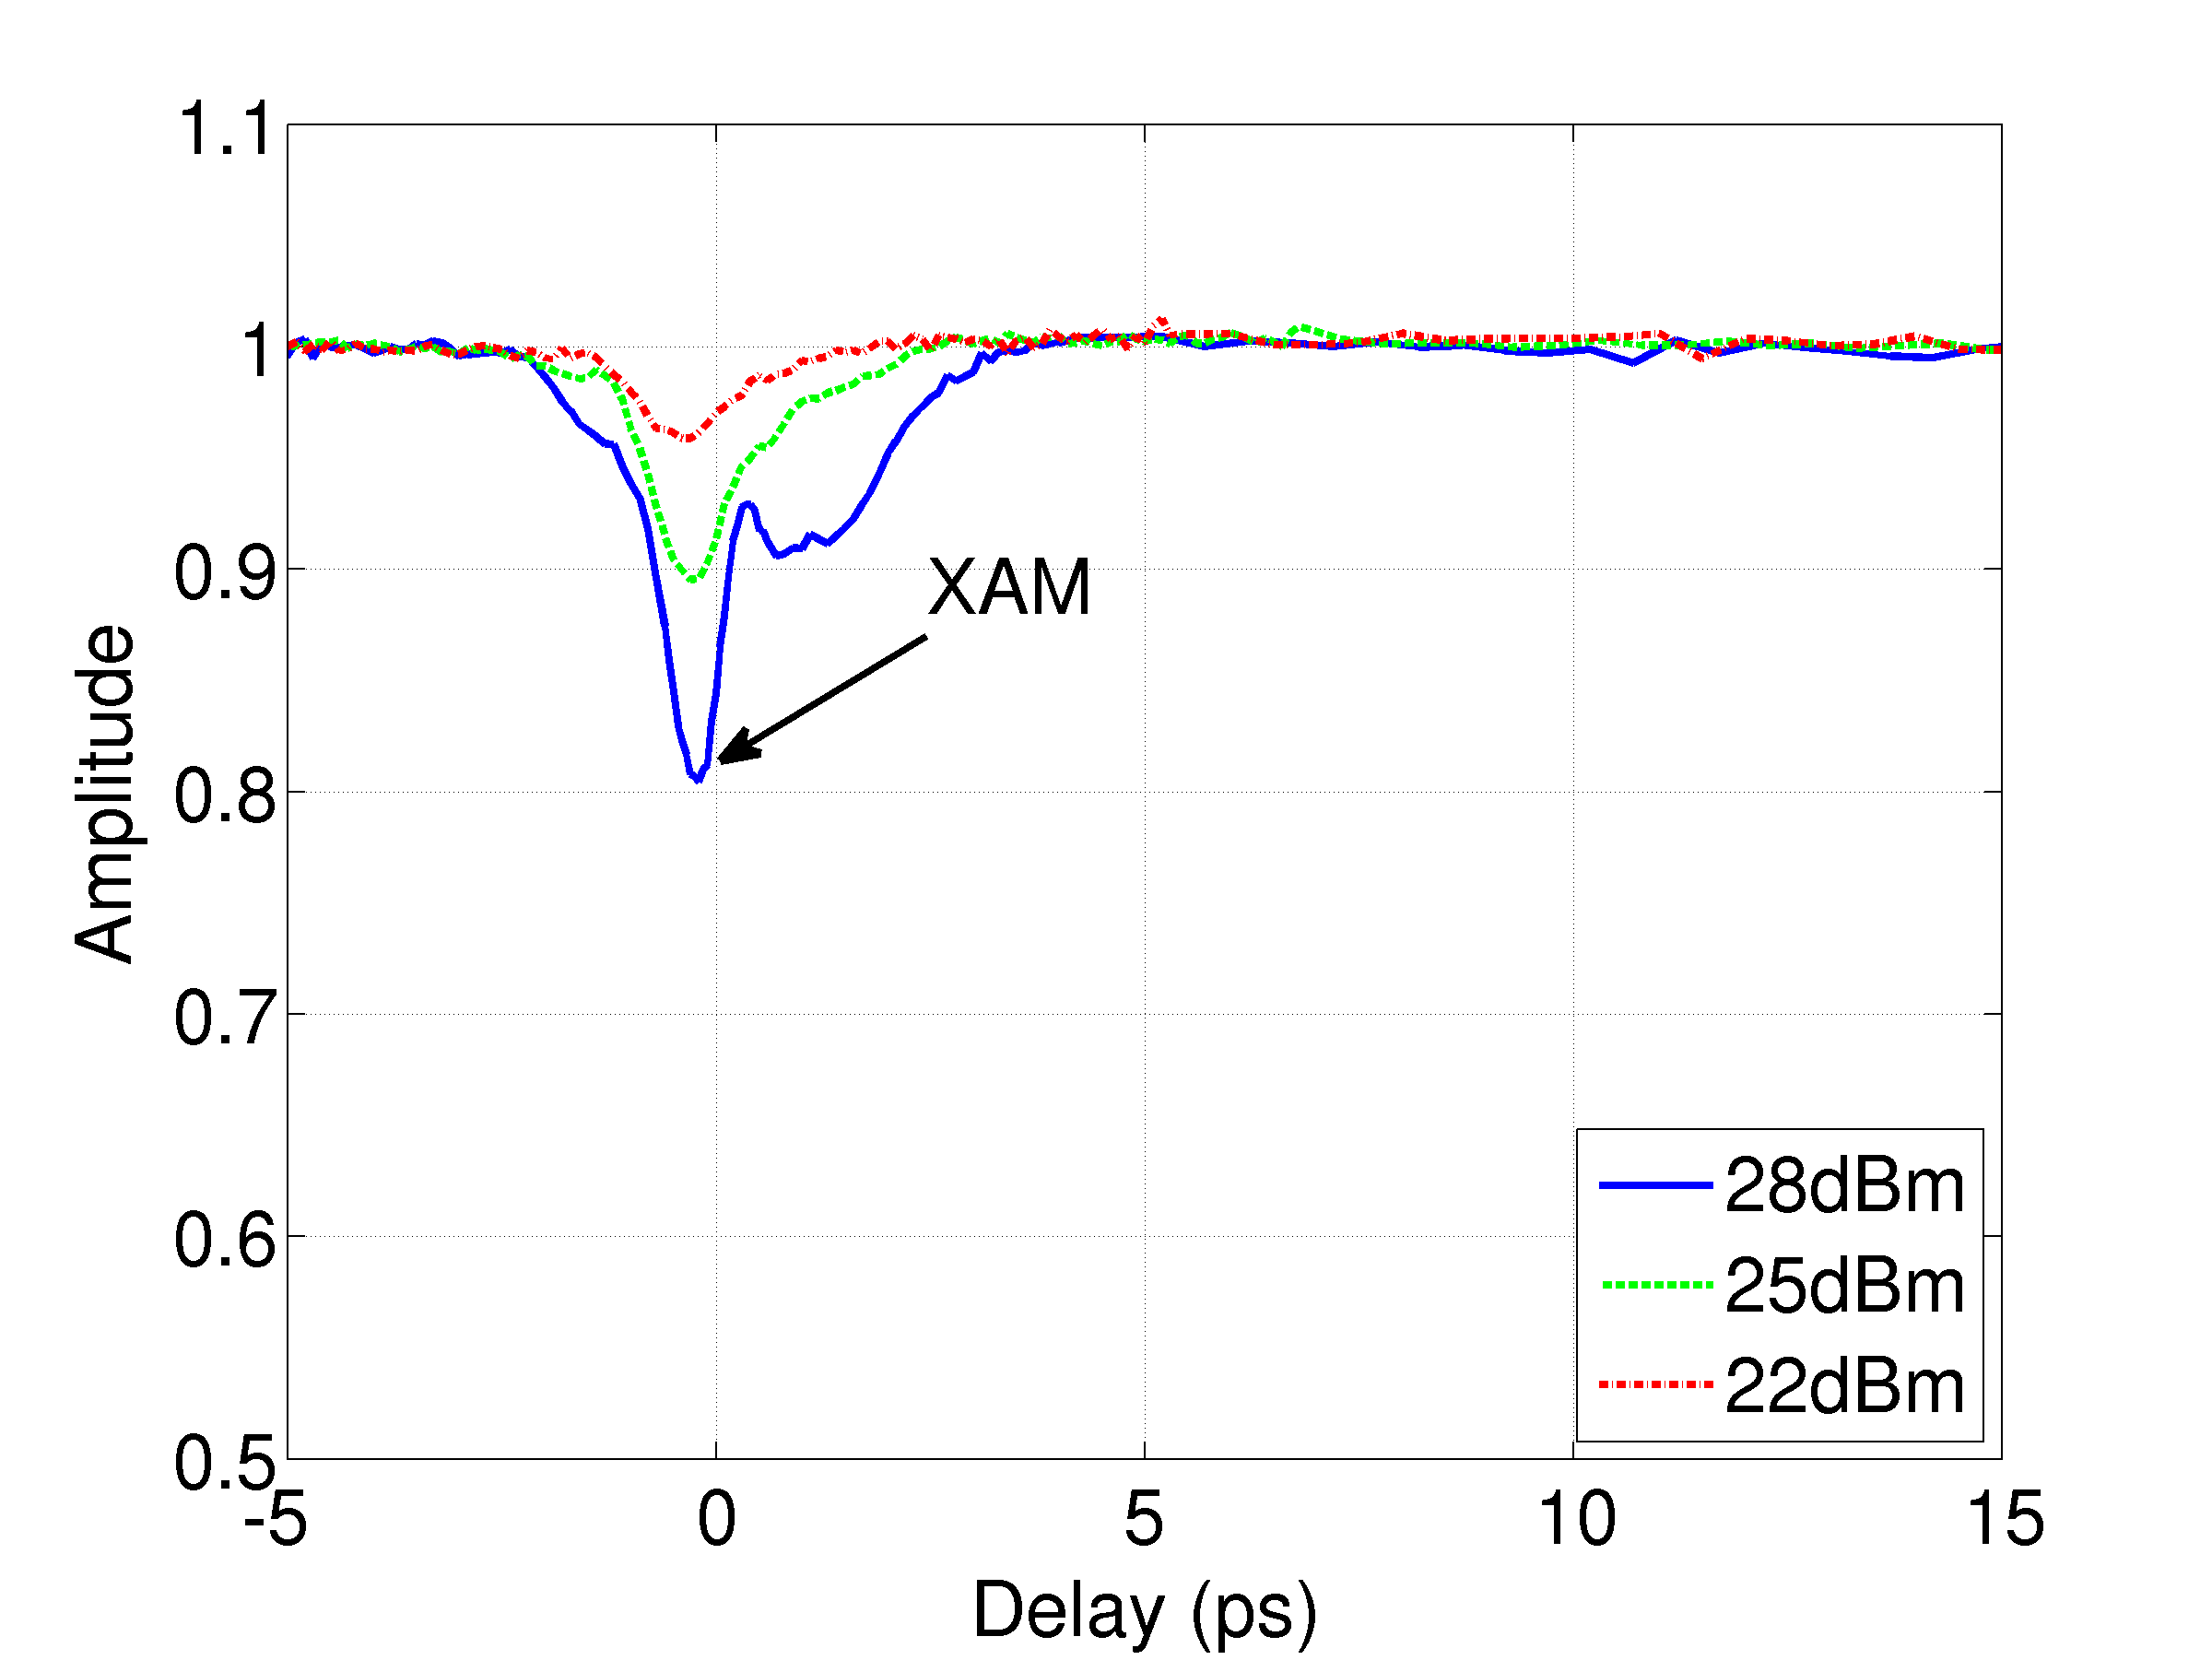
\includegraphics[width=0.49\textwidth]{ntc02amp}
    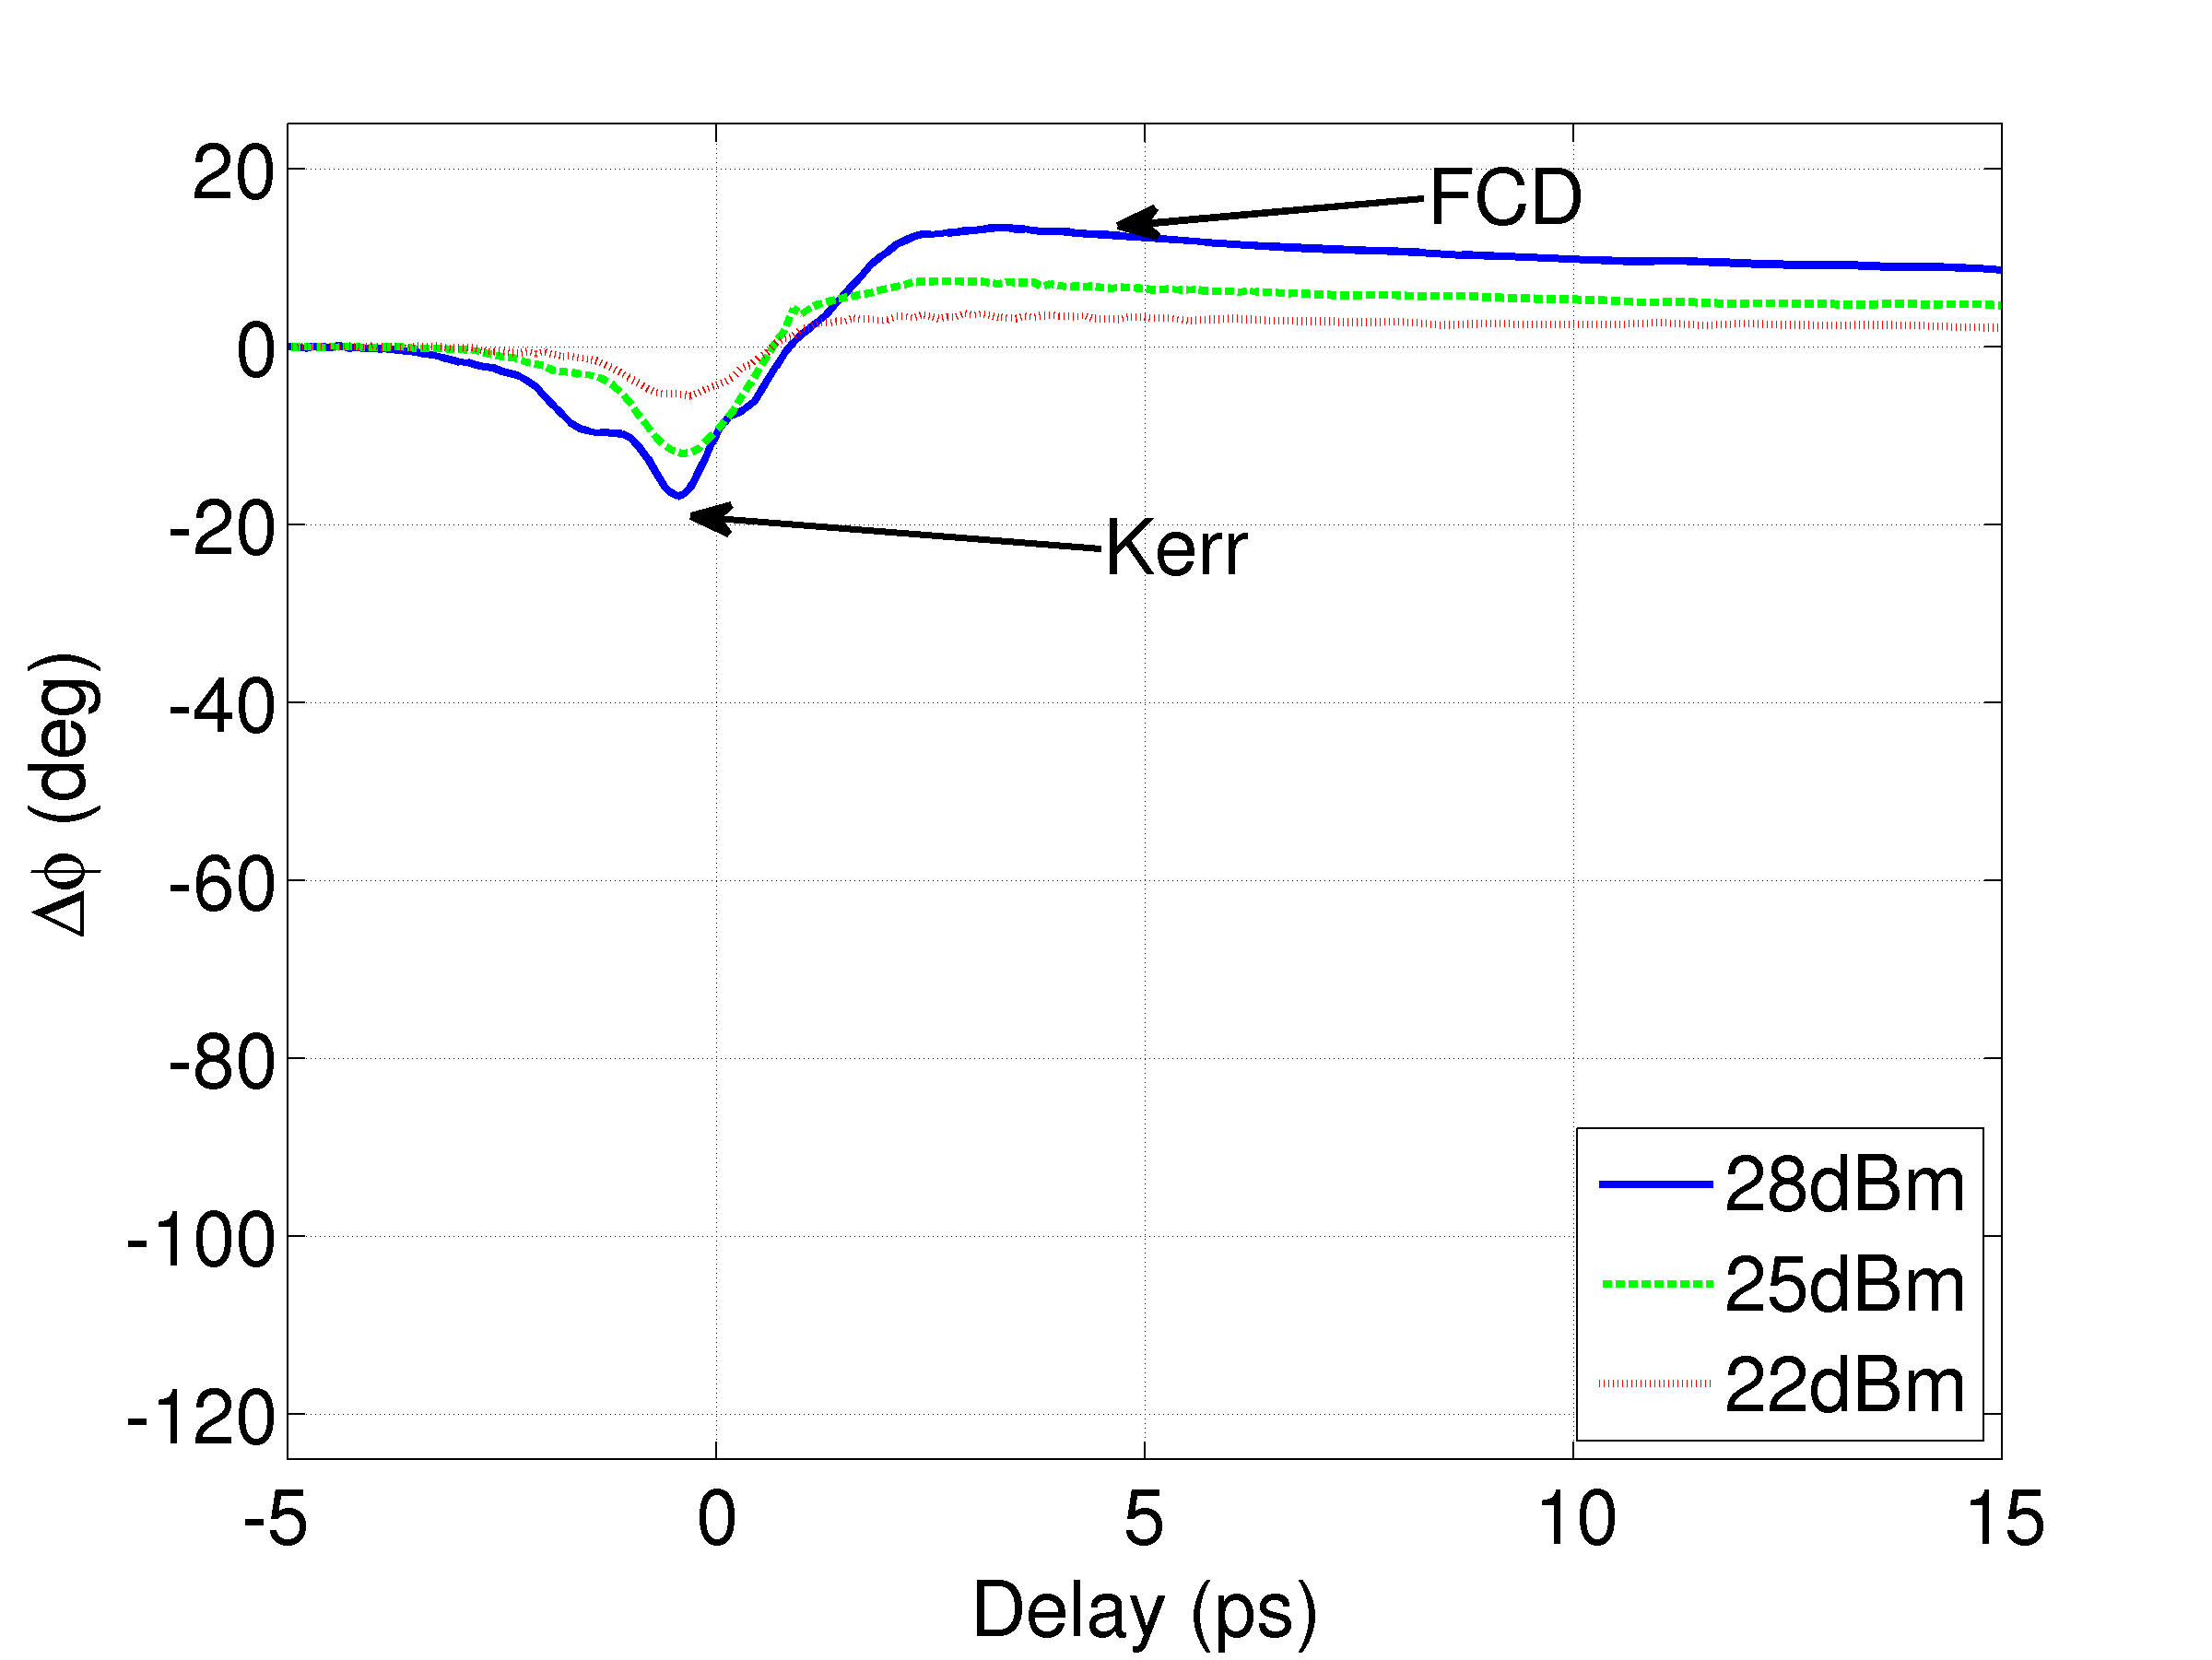
\includegraphics[width=0.49\textwidth]{ntc02phase}
    \caption{Sample response for different pump peak powers in the waveguide. Top: phase shift produced in probe pulse versus pump delay time (FCD: Free-carrier dispersion). Bottom: amplitude variation in the probe (XAM: cross absorption modulation).}
    \label{fig:ntc02TimeResSwitching}
\end{figure}

Fitting the carriers decay time to a double exponential, we can clearly observe two tendencies with different recombination times. One of them is very fast (8ps time constant) whereas the other is much slower (123 ps). (See Fig.~\ref{fig:zoomTimeResNtc02Switching}). Carrier recombination time in Si waveguides is usually reported to be in the ns range \cite{Almeida2004b,Xu2007}, so we attribute this fast response to surface defects in the waveguide.

\begin{figure}[htb]
    \centering
    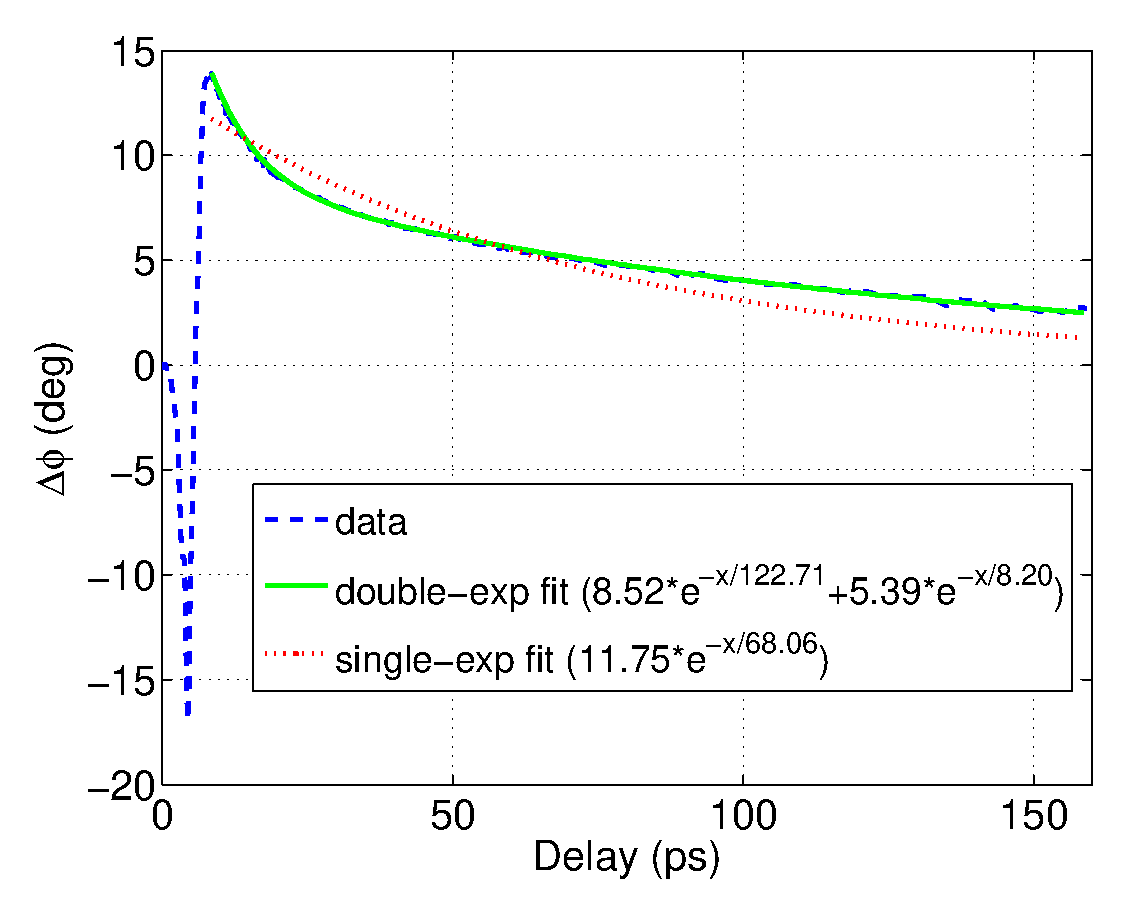
\includegraphics[width=\fWidth\textwidth]{ntc02phase_exp_fit}
    \caption{Panoramic view of the phase response in Fig.~\ref{fig:ntc02TimeResSwitching} showing the free-carriers decay. We use a two-exponential fit to simulate two very different recombination times, as a sigle-exponential fit is not able to follow both tendencies.}
    \label{fig:zoomTimeResNtc02Switching}
\end{figure}


\subsection{Switching experiment}
Figure \ref{fig:ntc02switching} shows the result of the second experiment, which is the demonstration of all-optical switching \cite{Oton}.The carrier dispersion effect produces a phase response, which is converted into intensity modulation by using a micro-ring resonator. As the resonance position blue-shifts when the carriers are excited, and the probe is tuned to the resonance, this shift produces an intensity modulation which is measured with the photo-diode. Using only 85~mW of pump peak power, the extinction ratio is 10.2~dB and the 1/e recovery time is 150~ps, which is close to the decay time observed in the phase-sensitive experiment. Depending on which point of the resonances we tune our CW laser we obtain positive (laser in the minimum of the resonance) or negative pulses (CW laser next to the resonance).  


\begin{figure}[htb]
    \centering
    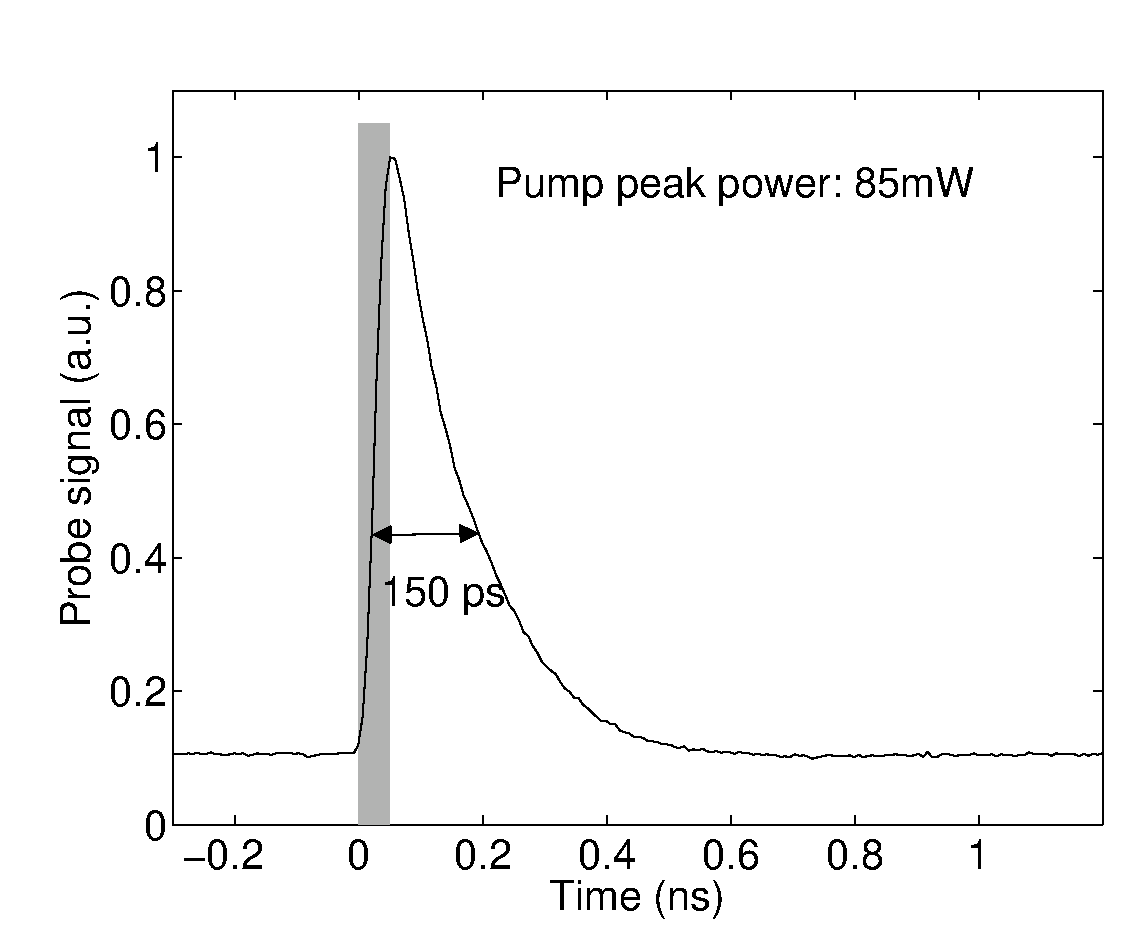
\includegraphics[width=0.49\textwidth]{pos_pulse_big}
    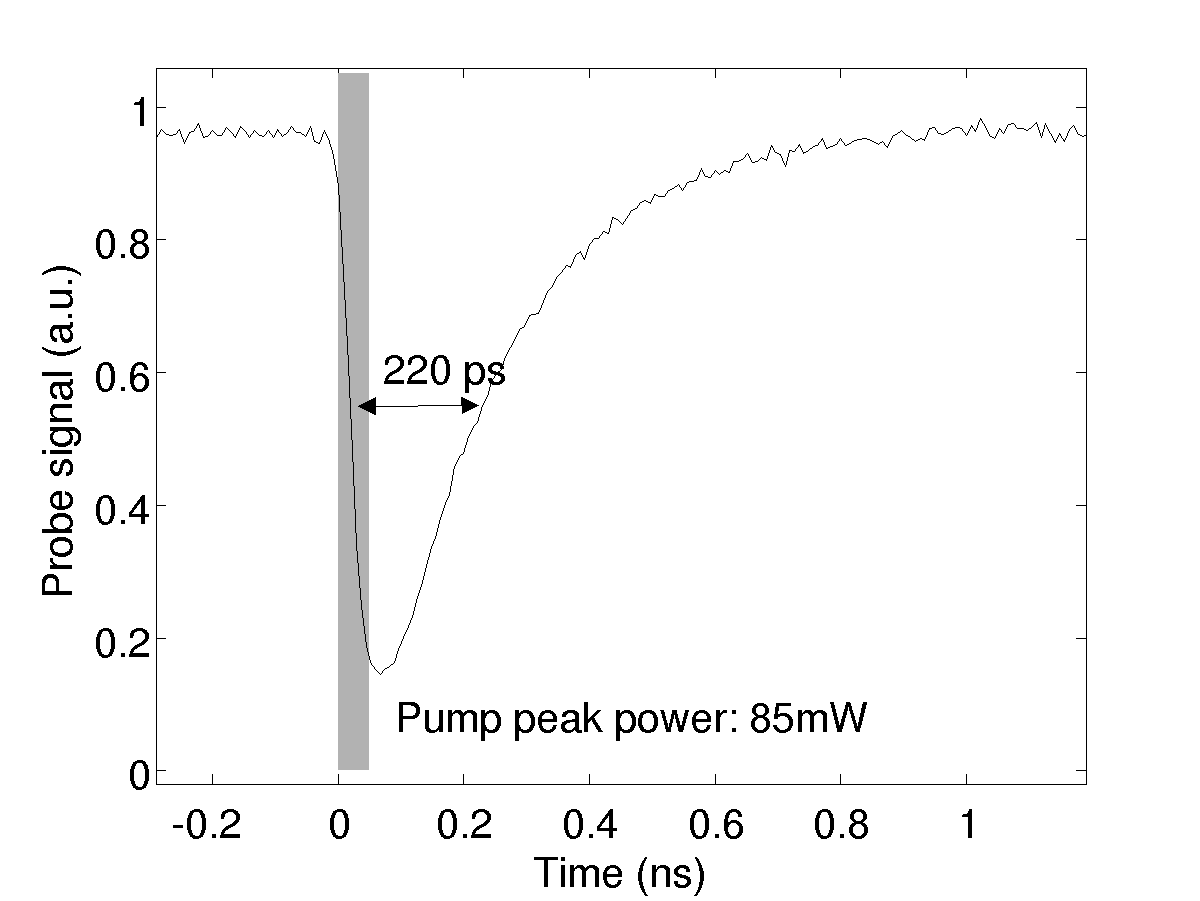
\includegraphics[width=0.49\textwidth]{neg_pulse_big}
    \caption{Variation of the probe signal when both pump and probe are resonant with two different modes of the microring. The grey box marks the pump duration. Depending on which point of the resonances we tune our CW laser we obtain positive (left figure) or negative pulses (right figure).}
    \label{fig:ntc02switching}
\end{figure}

\section{Conclusion}
We have characterized the dynamics of the nonlinear response of a Si waveguide with a time-resolved phase-sensitive pump and probe technique. The Kerr and XAM effects are clearly distinguished from the carrier dispersion effect. The carrier decay follows a double exponential decay with constants 8~ps and 122~ps, which is faster than values reported elsewhere. This fast decay time has allowed the fabrication of an all-optical switch with 10~dB extinction ratio and 150~ps recovery time, by using only 85~mW of pump peak power.

\section*{Acknowledgements}
This work has been sponsored by the Spanish Science and Innovation Ministry through SINADEC (TEC2008-06333) and DEMOTEC (TEC2008-06360) contracts and by Generalitat Valenciana through PROMETEO-2010-087R\&D Excellency Program (NANOMET).


\begin{thebibliography}{1}

\bibitem{Soref2006}
Richard Soref.
\newblock {The past, present, and future of silicon photonics}.
\newblock {\em IEEE Journal of Selected Topics in Quantum Electronics},
  12(6):1678--1687, 2006.

\bibitem{Oton}
C~J Oton, J~Matres, J~Herrera, and P~Sanchis.
\newblock 150 ps all-optical switching in silicon microring resonators.
\newblock In {\em European Conference on Integrated Optics}, 2010.

\bibitem{Oton2010}
C~J Oton, J~Matres, A~Martinez, P~Sanchis, J~P Colonna, C~Ratin, J~M Fedeli,
  and J~Marti.
\newblock {Ultrafast all-optical logic gates with silicon nanocrystal-based
  slot waveguides}.
\newblock In {\em Group IV Photonics (GFP), 2010 7th IEEE International
  Conference}, pages 171--173, 2010.

\bibitem{Turner-Foster2010}
Amy~C Turner-Foster, Mark~a Foster, Jacob~S Levy, Carl~B Poitras, Reza Salem,
  Alexander~L Gaeta, and Michal Lipson.
\newblock {Ultrashort free-carrier lifetime in low-loss silicon
  nanowaveguides.}
\newblock {\em Optics Express}, 18(4):3582--91, February 2010.

\bibitem{heebner2007optical}
John Heebner, Rohit Grover, and Tarek Ibrahim.
\newblock {\em {Optical microresonators: theory, fabrication, and
  applications}}.
\newblock Springer, 2007.

\bibitem{Almeida2004b}
Vilson R~VR Almeida, Carlos~A Barrios, Roberto~R Panepucci, and Michal Lipson.
\newblock {All-optical control of light on a silicon chip.}
\newblock {\em Nature}, 431(7012):1081--1084, 2004.

\bibitem{Xu2007}
Qianfan Xu and Michal Lipson.
\newblock {All-optical logic based on silicon micro-ring resonators.}
\newblock {\em Optics Express}, 15(3):924--9, February 2007.

\end{thebibliography}

\chapter{Paper:~Ultrafast all-optical logic gates with Si-nanocrystal slot}
\label{ch:paperLogicGates}

What prevented us from using more power or presenting an Eye pattern in high speed switches and logic gates is the generation of free-carriers in Silicon waveguides, which alters the level of zero when several pulses arrive.
To solve this problem, there are several strategies. The most common is to create a reverse polarized PN junction to sweep carriers~\cite{Turner-Foster2010}, but it complicates the fabrication and increases the power consumption.

We proposed to enhance the Kerr response by introducing silicon nanocrystals, with very high $\chi^3$, in a horizontal slot configuration. Using this structure we demonstrated an all-optical logic gate with ultrafast switching time ($<40$~ps). In this paper I participated in the experimental measurements and data analysis together with C. Oton. The paper was presented in the IEEE Group IV Photonics, and the reference is the following:


\vspace{1.5cm}
C. J. Oton, J. Matres, A. Martinez, P. Sanchis, J. P. Colonna, C. Ratin, J. M. Fedeli, and J. Marti, “Ultrafast all-optical logic gates with silicon nanocrystal-based slot waveguides”, in Group IV Photonics (GFP), 2010 7th IEEE International Conference, 2010, pp. 171–173.

\newpage
\begin{center}
\section*{Ultrafast all-optical logic gates with silicon nanocrystal-based slot waveguides}
{C. J. Oton$^{1}$, J. Matres$^{1}$,  A. Mart\'inez$^1$, P. Sanchis$^1$,J. P. Colonna$^2$, C. Ratin$^2$, J.M. F\'ed\'eli$^2$ and J. Mart\'i,$^1$} 
\end{center}

\noindent
\textit{$^1$ Nanophotonics Technology Center, Universidad Polit\'ecnica de Valencia, Camino de Vera s/n, 46022, Valencia, Spain\\
$^2$CEA LETI, Minatec Campus, Grenoble 38054, France}


\textbf{Abstract} \\
\noindent
We report an ultrafast ($<40$~ps) all-optical XOR logic gate based on a silicon nanocrystal-based horizontal slot waveguide.
The device consists of a Mach-Zehnder interferometer with three input ports, and is driven by $\approx 200~$mW peak power.


\section{Introduction}
Silicon photonics has recently become a subject of intense research, particularly during the last years, when industries have started to develop devices which are now becoming competitive with other technologies. During the last few years, there have been significant advances in nonlinear devices such as all-optical switches, routers, and logic gates. These devices usually take advantage of the free carrier dispersion (FCD) effect produced by carriers generated through two-photon absorption (TPA) mechanisms. The main issue with these devices is the speed, dominated by a carrier recombination time which is usually in the order of 1 ns. Different approaches have been proposed to increase the speed, the most successful one being carrier depletion through a p-i-n junction,\cite{Turner-Foster2010} although it still has a bandwidth limitation.
On the other hand, the nonlinear Kerr effect is more appealing than the carrier-related nonlinearities, as the former is instantaneous thus there is no intrinsic bandwidth limitation. However, in standard silicon waveguides, the carrier-related effects take place at lower powers than the Kerr effect, so the ultrafast Kerr response gets masked. Therefore, other materials have to be combined with silicon to attain a more intense Kerr response. Polymers have been proposed as suitable candidates,\cite{Koos2009} but these materials involve non-CMOS processes and impose a temperature limitation too. Silicon nanocrystal-based waveguides only require CMOS processes and have a very high nonlinear coefficient~\cite{Spano2009}. In this paper we show experimental results of an ultrafast all-optical XOR logic gate in a Mach-Zehnder interferometer (MZI) based on this approach.


\section{Fabrication}
The layer responsible for the nonlinear Kerr effect is PECVD-grown silicon-rich silica (SiOx), which is annealed at $1200^\circ$C for 1~h so that it can form silicon nanoclusters. However, in the sample presented here, the amount of silicon excess is too low to measure it with precision (probably less than 1\%). In order to enhance the nonlinear effect, this layer was sandwiched between two silicon channels in a horizontal slot configuration~\cite{Jordana2007}. To fabricate such a geometry, a 100~nm layer of SiOx followed by a 220~nm polysilicon layer were deposited on top of a standard SOI wafer with 220~nm Si layer. The waveguides were dry-etched to form 500~nm-wide channels, and inverted tapers as in Ref.~\cite{Bakir2010} were added to the facets to facilitate the coupling. The whole layout was covered with silica. More details of the fabrication and material properties can be found in Ref.~\cite{Martinez2010}.


\section{Characterization}
Figure~\ref{fig:setupLogicGate} sketches the setup employed for the nonlinear characterization. A low-power cw probe laser was launched into the central branch of an asymmetric MZI, while two different high power pulse patterns were coupled to each branch of the MZI. A standard 250~$\mu$m-separated flat fiber array was used to couple to the 3-input-port MZI. The XOR behavior of the device comes from the fact that equal inputs in the branches keep the MZI balanced, thus there is no response, while different inputs unbalance the interferometer, generating a response in the probe signal. The MZI also had microring resonators in each branch, although in this experiment their effect is not observable because the wavelengths were chosen to be far from the resonances. Propagation losses were less than 5~dB/cm.

\begin{figure}[htb]
    \centering
    \includegraphics[width=1.0\textwidth]{setupLogicGate}
      \caption{Experimental setup for the characterization of the optical logic gate. Triangles represent Er-doped fiber amplifiers with an ASE filter. A fiber array was used to simultaneously couple the light to the three inputs of the MZI.}
    \label{fig:setupLogicGate}
\end{figure}


The wavelength of the pump was set to 1560~nm, although it does not particularly matter in the performance of the device, as there are no interference fringes on that input, as shown in Fig.~\ref{fig:spectrumXor}. The wavelength of the probe signal does matter, as the intentional asymmetry of the branches produces fringes which allow us to set the initial working point at any point of the fringe. The wavelength chosen was 1546.27~nm, where the slope of that particular fringe was maximum, in order to get the maximum response. This working point produces positive (negative) pulses in the probe signal when pulses are coupled to the branch A (B), as shown in Fig.~\ref{fig:ultrafastXor}. As branch A is shorter than branch B, this means that the effective index increases in presence of the pump, which means that the Kerr coefficient is positive, and rules out the generation of carriers as the cause of the fast nonlinearity. When both branches are simultaneously excited, the phase change is identical in both 
branches, thus no response is observed. Peak powers in the coupling fiber was only 500~mW, which becomes 200~mW after 4~dB estimated coupling loss, and produced $\approx$1dB modulation depth, as shown in Fig.~\ref{fig:ultrafastXor}.
Although the ultrafast response is produced by a Kerr effect, which is instantaneous, there were also carriers generated by TPA which introduced a much slower response too ($>1$~ns). This effect is negligible when short trains of pulses are sent, but when a realistic telecom signal is launched, it generates a fluctuating baseline which prevents an error-free performance. This is a well-known issue in any silicon waveguide where carriers are generated, and can be overcome for example by introducing a carrier depletion mechanism~\cite{Turner-Foster2010}. This would also allow coupling higher powers to the device, thus achieving a higher modulation extinction ratio.

\begin{figure}[htb]
    \centering
    \includegraphics[width=0.8\textwidth]{spectrumXor}
      \caption{Spectrum of the asymmetric MZI of 15~mm length and 350~$\mu$m path difference, for the three input branches. Pump and probe wavelengths are indicated with arrows.}
    \label{fig:spectrumXor}
\end{figure}


\begin{figure}[htb]
    \centering
    \includegraphics[width=0.8\textwidth]{ultrafastXor}
      \caption{Ultrafast probe signal when a train of two bits separated 100~ps is sent through branches A and B (top, blue), just A (middle, green) and just B (bottom, red).}
    \label{fig:ultrafastXor}
\end{figure}


\section{Conclusions}
We report the experimental characterization of an all-optical XOR logic gate on a silicon-nanocrystal slot waveguide. This geometry provides an enhanced Kerr effect, enabling ultrafast ($<40$~ps) switching times. The device is a Mach-Zehnder interferometer with 3 input ports, and achieves $\approx 1$~dB modulation depth by using optical peak powers of $\approx 200$~mW.

\section*{Acknowledgments}
We acknowledge financial support from the EU project PHOLOGIC (FP6-IST-NMP-017158) and from the Spanish Ministry of Science and Innovation through contracts SINADEC (TEC2008-06333) and DEMOTEC (TEC2008-06360).

\begin{thebibliography}{1}

\bibitem{Turner-Foster2010}
Amy~C Turner-Foster, Mark~a Foster, Jacob~S Levy, Carl~B Poitras, Reza Salem,
  Alexander~L Gaeta, and Michal Lipson.
\newblock {Ultrashort free-carrier lifetime in low-loss silicon
  nanowaveguides.}
\newblock {\em Optics Express}, 18(4):3582--91, February 2010.

\bibitem{Koos2009}
C~Koos, P~Vorreau, T~Vallaitis, P~Dumon, W~Bogaerts, R~Baets, B~Esembeson,
  I~Biaggio, T~Michinobu, F~Diederich, W~Freude, and J~Leuthold.
\newblock {All-optical high-speed signal processing with silicon – organic
  hybrid slot waveguides}.
\newblock {\em Nature Photonics}, 3(April):1--4, 2009.

\bibitem{Spano2009}
R~Spano, N~Daldosso, M~Cazzanelli, L~Ferraioli, L~Tartara, J~Yu, V~Degiorgio,
  E~Giordana, J~M Fedeli, and L~Pavesi.
\newblock {Bound electronic and free carrier nonlinearities in Silicon
  nanocrystals at 1550nm.}
\newblock {\em Optics Express}, 17(5):3941--3950, 2009.

\bibitem{Jordana2007}
E~Jordana, J.-M. Fedeli, P~Lyan, J~P Colonna, P~E Gautier, N~Daldosso,
  L~Pavesi, Y~Lebour, P~Pellegrino, B~Garrido, J~Blasco, F~Cuesta-Soto,
  P~Sanchis, Grenoble Cedex, and De~Barcelona.
\newblock {Deep-UV Lithography Fabrication of Slot Waveguides and Sandwiched
  Waveguides for Nonlinear Applications}.
\newblock In {\em Group IV Photonics, 2007 4th IEEE International Conference},
  number~1, pages 1--3, 2007.
  
\bibitem{Bakir2010}
B. Ben Bakir, A. V de Gyves, R. Orobtchouk, P. Lyan, C. Porzier, A. Roman, and J.-M. Fedeli
\newblock {Low-loss ($<~1$ dB) and polarization-insensitive edge fiber couplers
  fabricated on 200-mm silicon-on-insulator wafers}.
\newblock {\em IEEE Photonics Technology Letters}, 22(11):739--741, 2010.

\bibitem{Martinez2010}
Alejandro Mart\'{\i}nez, Javier Blasco, Pablo Sanchis, Jos\'{e}~V Gal\'{a}n,
  Jaime Garc\'{\i}a-Rup\'{e}rez, Emmanuel Jordana, Pauline Gautier, Youcef
  Lebour, Sergi Hern\'{a}ndez, Romain Guider, Nicola Daldosso, Blas Garrido,
  Jean~Marc Fedeli, Lorenzo Pavesi, Javier Mart\'{\i}, and Rita Spano.
\newblock {Ultrafast all-optical switching in a silicon-nanocrystal-based
  silicon slot waveguide at telecom wavelengths.}
\newblock {\em Nano letters}, 10(4):1506--11, April 2010.

\end{thebibliography}

\chapter{Paper:~Low TPA and free-carrier effects in Si-nanocrystal slot}
\label{ch:articleTimeRes}
\pagestyle{plain}

In the previous chapter, ultrafast Si-nanocrystal-based optical logic gates were demonstrated. However, a proper quantification of the carrier effects and TPA was missing. In order to characterize separately all these nonlinear effects, we set up an advanced experiment capable of measuring the ultrafast nonlinear response in phase and amplitude. We performed measurements on a Si-nanocrystal slot sample and compared it to standard Si strip waveguides, where we were able to quantitatively conclude the better performance of the silicon-nanocrystal slot through its nonlinear figure-of-merit.

The paper was the result of a collaboration between my group in UPV, the group of Dr. I. Cristiani, in Uniersity of Pavia, and CEA LETI in Grenoble, France, who fabricated the samples. My personal contribution to the work is the following: I made the experimental measurements, together with C. Lacava; I analyzed the data and drafted the paper. Simulations of the waveguides were done by Guillem Ballesteros and Paolo Minzioni independently, reaching the same results. The paper was published in Optics Express, and the reference is the following:

\vspace{1.5cm}

J Matres, C Lacava, G C Ballesteros, P Minzioni, I Cristiani, J Marti, J M Fedeli, and C J Oton. Low TPA and free-carrier effects in silicon nanocrystal-based horizontal slot waveguides. Opt. Express, 20(21):23838–23845, October 2012

\newpage
\begin{center}
\section*{Low TPA and free-carrier effects in silicon nanocrystal-based horizontal slot waveguides}
{J. Matres,$^{*,1}$ C. Lacava,$^2$ G. C. Ballesteros,$^1$ P. Minzioni,$^2$ I. Cristiani,$^2$ J.~M.~F\'ed\'eli,$^3$ J. Mart\'i,$^1$ and C. J. Oton,$^1$} 
\end{center}
\noindent
\textit{$^1$ Nanophotonics Technology Center, Universidad Polit\'ecnica de Valencia, Camino de Vera s/n, 46022, Valencia, Spain\\
$^2$Dipartimento di Ingegneria Industriale e dell'Informazione, Universita di Pavia, Via Ferrata 1, 27100, Pavia, Italy\\
$^3$CEA LETI, Minatec Campus, Grenoble 38054, France}

\begin{center}
{$^*$joamatab@ntc.upv.es}

%%%%%%%%%%%%%%%%%%% abstract and OCIS codes %%%%%%%%%%%%%%%%
%% [use \begin{abstract*}...\end{abstract*} if exempt from copyright]

\end{center}


%\begin{abstract}
\textbf{Abstract} \\
\noindent
We present the characterization of the ultrafast nonlinear dynamics of a CMOS-compatible horizontal-slot waveguide with silicon nanocrystals.
Results are compared to strip silicon waveguides, and modeled with nonlinear split-step calculations.
The extracted parameters show that the slot waveguide has weaker carrier effects and better nonlinear figure-of-merit than the strip waveguides. 
%\end{abstract}

\begin{center}
{(190.0190) Nonlinear optics; (130.0130) Integrated optics; (320.0320) Ultrafast optics; (160.4330) Nonlinear optical materials.}
\end{center}
%(220.0220) Optical design and fabrication; (230.5750) Resonators; (230.3990) Microstructure devices; (250.5300) Photonic Integrated Circuits.}

%%%%%%%%%%%%%%%%%%%%%%% References %%%%%%%%%%%%%%%%%%%%%%%%%



\section{Introduction}
Nonlinear silicon-based photonic devices can introduce key functionalities for on-chip optical signal processing and routing. In the last years, many different nonlinear silicon devices have been reported, such as all-optical modulators~\cite{Almeida2004b}, wavelength converters~\cite{Lee2009,Driscoll2010}, demultiplexers~\cite{Koos2009}, format converters~\cite{Astar2010}, etc.
These nonlinear devices can be based either on free carriers or on the bound-electron Kerr coefficient.
In pure silicon waveguides, the Kerr effect is usually hindered by more intense and longer-lasting free-carrier dispersion (FCD)~\cite{Foster2008,Osgood2009}. However, it is often desirable to exploit the Kerr effect, as its temporal response is instantaneous (thus allowing high-speed operation) and it enables parametric conversion and amplification. In order to increase the Kerr coefficient and reduce carrier effects in silicon waveguides, a slot-type geometry~\cite{Almeida2004} was proposed~\cite{Sanchis2007,Koos2007a,Zhang2010,Rukhlenko2012}, where a thin layer of a low-index material material with high nonlinear coefficient is sandwiched between two silicon channels.
A vertical slot geometry was also demonstrated to allow the introduction of an organic polymer, and this device showed optical 160~Gb/s demultiplexing capabilities~\cite{Koos2009}; however, these materials involve non-CMOS processes and impose strict temperature limitations.
On the other hand, silicon-nanocrystal-based horizontal slot waveguides only require CMOS processes, and have recently demonstrated ultrafast all-optical modulation capabilities and good nonlinear properties~\cite{Spano2009, Martinez2010a, Oton2010, Trita2011}.
In this paper, we study the nonlinear ultrafast dynamics of this type of waveguide, where we show that the effect of carriers is greatly reduced as compared to silicon channel waveguides. We also report quantitative measurements of nonlinear absorption of these waveguides.
Finally we show simulation results which fit the experimental data and provide estimations of the nonlinear parameters and figures of merit of the waveguides.


\section{Fabrication}
Slot samples were fabricated starting from silicon--on--insulator (SOI) wafers with 220~nm Si thickness.
On top of the Si layer, a 100~nm--thick layer of silicon--rich silica ($ \mathrm{SiO_x} $) was grown by plasma-enhanced chemical vapor deposition (PECVD) using a gas ratio of $[N_2O/SiH_4]=180/20$ subsequently annealed at $1000^\circ$ ~in $ \mathrm{N}_2 $ ambient for 210~s.
The nominal amount of silicon excess was 16\% and Silicon-nanocrystals had an average size of 4~nm.
The value of Si-excess was determined by using the X-ray photoelectron spectroscopy (XPS) and the average size of formed Si-nc was determined by means of the Energy Filtered Transmission Electron Microscopy EFTEM. Both these techniques are well described in~\cite{Garcia2004}.
The top layer of the slot structure was fabricated using an hydrogenated amorphous silicon layer.
Annealing temperature was set to $400^\circ$ C to avoid the silicon crystallization process.
The nano-slot fabrication process was previously optimized in order to obtain a low-loss and high nonlinear performance as described in~\cite{Jordana2007}.
Waveguides were patterned with deep-UV lithography and etched down to the buried oxide to form channels as the ones reported in~\cite{Martinez2010a, Trita2011}.
The whole layout was covered with silica after the etching process as shown in Fig.~\ref{fig:semSlot}.
On the other hand, two Si strip waveguides were fabricated for comparison, always starting  from SOI wafers patterned with deep-UV lithography.
Their dimensions were $445\times220$~nm for transverse-electric (TE) polarization and $485\times220$~nm for transverse-magnetic (TM) polarization, both with a length of 25~mm.
The slot waveguide, where the TM-polarized mode was excited to exploit the E-field magnification effect in the slot region, was 7~mm long.


\begin{figure}[htb]
\centering
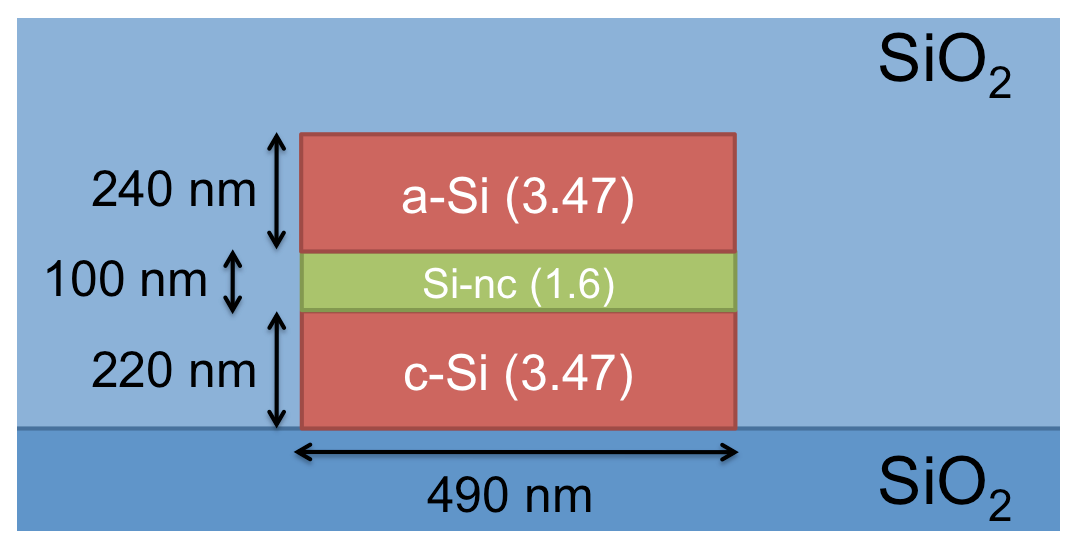
\includegraphics[width=0.42\textwidth]{slot5}%0.6
\caption{Silicon-nanocrystals (Si-nc) slot waveguide schema. Top made of amorphous silicon (a-Si) and bottom of crystalline silicon (c-Si).
Refractive index of the Si-nc layer was measured from a thick Si-nc sample using the m-lines technique.}
\label{fig:semSlot}
\end{figure}


\section{Nonlinear loss measurements: Im$ (\gamma) $}
\label{sec:imGammaTimeRes}
First, we characterized the nonlinear loss in all the samples under test.
Two-photon absorption (TPA) is a well-known process in silicon waveguides, and can be considered as the imaginary part of the gamma coefficient using the differential equation derived in \cite{Mizrahi}:

\begin{equation}
\frac{dP}{dz} = -\alpha P(z) - 2|Im(\gamma)| P(z)^2 
\label{eq:differentialTPAtimeRes}
\end{equation}

where $P$ is the signal power through the waveguide, $\alpha$ is the linear loss of the waveguide, and Im$(\gamma)$ is the imaginary part of the $\gamma$ coefficient (we use the absolute value because we want to stress its loss character in the equation with a negative sign). 
The solution of the differential equation shown in Eq.~\ref{eq:differentialTPAtimeRes} after a distance $L$ is given by:

\begin{equation}
P(L) = \frac{e^{-\alpha_0 L}}{1+2|Im(\gamma)| L_{eff} P_0} P_0
\end{equation}

where $P_0$ is the input power in the waveguide and $ L_{eff} $ the effective length:

\begin{equation}
L_{eff} = \frac{1-e^{-\alpha_0L}}{\alpha_0}
\end{equation}


Therefore the impact of nonlinear losses ($T_{NL}^{-1}$) on the overall transmission can be calculated as the ratio between the transmission at low power ($T_{LP} = e^{-\alpha_0 L} $) and the transmission at high power ($T_{HP} = P(L)/P_0 $). In particular the inverse of $T_{NL}$ turns out to be a linear function of $P_0$:

\begin{equation}
T_{NL}^{-1} = \frac{T_{LP}}{T_{HP}} = 1+2|Im(\gamma)| L_{eff} P_0
\label{eq:transmissionLinearTimeRes}
\end{equation}

As a consequence, if we plot this ratio as a function of $P_0$, the slope of the curve can give us the two-photon absorption coefficient of the waveguide as in~\cite{Vallaitis2009}.
However, this equation is only valid for instantaneous transmission values.
We find that when a pulsed signal $P_0(t)$ is launched into the waveguide, the measured transmission is time averaged, so defining $ \tilde{T} $ as the integrated transmission along the duration of the pulse, the equivalent nonlinear loss $\tilde{T}_{NL}^{-1}$ can be expressed as:

                                                                \begin{equation}
                                                                        \tilde{T}_{NL}^{-1} = \frac{\tilde{T}_{LP}}{\tilde{T}_{HP}} = \frac{\int P_0(t)dt}{\int \frac{P_0(t)}{1+2|Im(\gamma)| L_{eff} P_0(t)} dt}
                                                                        \label{eq:transmissionIntegralTimeRes}
                                                                \end{equation}

If the pulsed signal has a rectangular shape, one can use Eq.~\ref{eq:transmissionLinearTimeRes}, but if the shape is different, the integral in Eq.~\ref{eq:transmissionIntegralTimeRes} must be solved, as the result differs significantly.
The reason for this variation is the fact that the flanks of the pulse are not affected as hardly by TPA as the peak.
Therefore, the overall energy transmission is higher than for the case of cw excitation.
For the particular case of a $sech^2$ shape, which corresponds to the output of our laser, emitting 1-ps pulses with a repetition rate of 20~MHz and a central wavelength of 1539~ nm, the time dependent power can be expressed by:

\begin{equation}
P_0(t)=P_{0 peak} sech^2 \left(\frac{t}{\tau}\right)
\label{eq:sech2timeRes}
\end{equation}

and substituting Eq.~\ref{eq:sech2timeRes} in Eq.~\ref{eq:transmissionIntegralTimeRes} and solving the integral, one obtains:

                                                                \begin{equation}
                                                                        \tilde{T}_{NL}^{-1}  = \frac{\tilde{T}_{LP}}{\tilde{T}_{HP}} \bigg|_{sech^2~shape}  = \frac{\sqrt{\delta({\delta + 1})}}{\ln(\sqrt{\delta}+\sqrt{\delta+1})} ~~\mathrm{where}~~  \delta = 2|Im(\gamma)| L_{eff} P_{0 peak}
                                                                        \label{eq:transmissionHypSecantTimeRes}
                                                                \end{equation}


We measured the $\tilde{T}_{LP}$ and $\tilde{T}_{HP}$ parameters by putting a variable attenuator at the laser output and using a power-meter.
The experimental results are shown in Fig.~2, together with the fitting curves obtained using Eq.~\ref{eq:transmissionHypSecantTimeRes} in order to extract the Im$(\gamma)$ parameter shown in Table \ref{tab:resultsArticleSlot}. 
It is worth noting that the Im$(\gamma )$ of slot waveguides is much lower than that of TE strip waveguides.
This can be easily explained considering that in the slot structure the main part of the optical field is confined within the region containing silicon oxide doped with silicon nanocrystals, which have a band-gap higher than that of crystalline Silicon as theoretically and experimentally demonstrated by several authors in the past years~\cite{Buuren98, Bassani, Daldosso2009}.
The low value of Im$(\gamma)$ measured in TM strip waveguide is due to the fact that the mode largely extends in the $\mathrm{SiO_2}$ cladding.

\begin{figure}[htb]
    \centering
    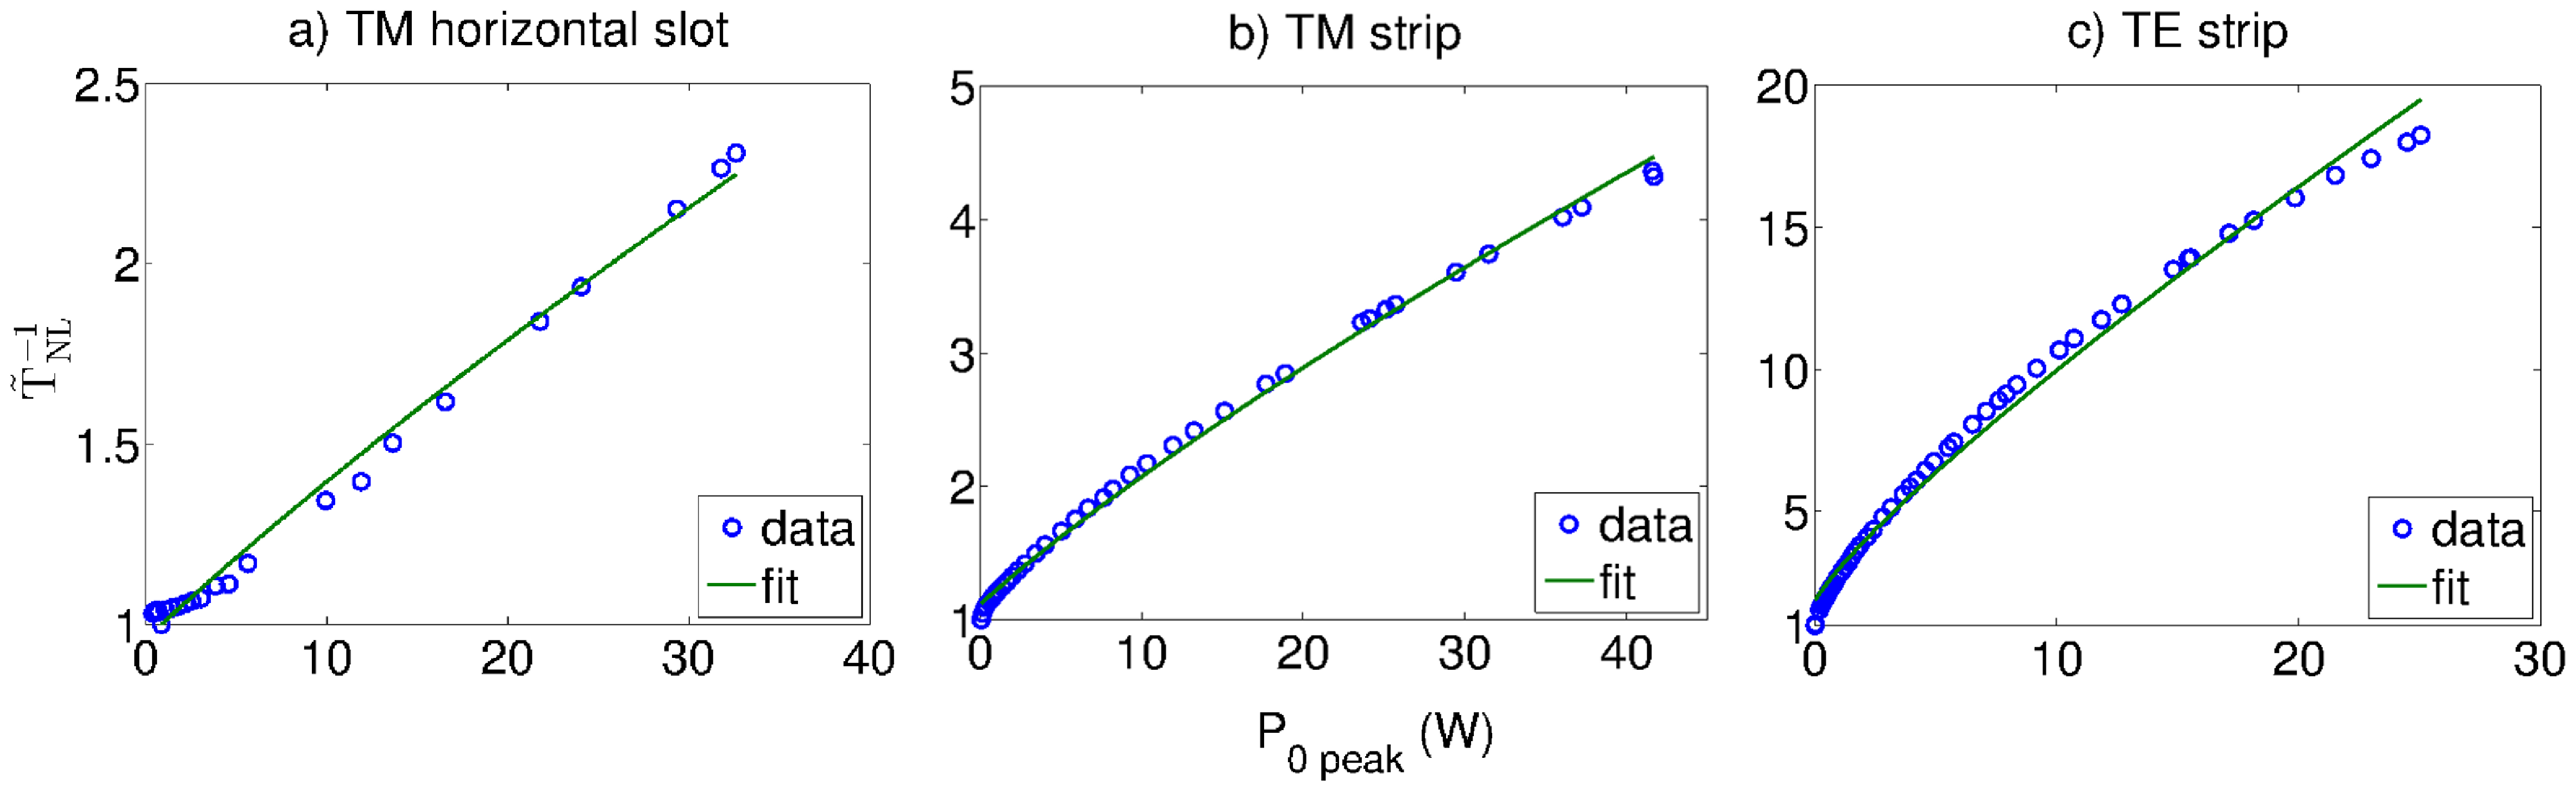
\includegraphics[width=1.0\textwidth]{imGamma_slot_TM_TE_v6}
     \caption{Transmission versus waveguide peak power (note the difference in the y-scale among the three plots). Solid line shows the fit for $ sech^2 $ pulses using Eq.~\ref{eq:transmissionHypSecantTimeRes}.}
    \label{fig:imGammaSamples}
\end{figure}



\section{Time-resolved measurements}
Time resolved measurements were performed in order to distinguish Kerr and TPA from carrier effects, using the technique described in \cite{Vallaitis2008}.
The set-up is shown in Fig.~\ref{fig:setupTimeResTimeRes}. We split the 1~ps pulse into three pulses: the most intense acts as a pump, while the two weaker pulses (reference and probe) are frequency shifted by two acousto-optic modulators (respectively by 80~MHz and 80.04~MHz ) and recombined with a fixed probe-to-reference delay of 10~ns.
All the pulses are then coupled inside the waveguide under test and the time-delay between probe pulse and pump pulse is changed by means of a variable delay line.
At the output, the probe and reference pulses are re-synchronized by a 10~ns delay-line and their beating signal is recovered by a lock-in amplifier.

                                \begin{figure}[htb]
                                         \centering
                                         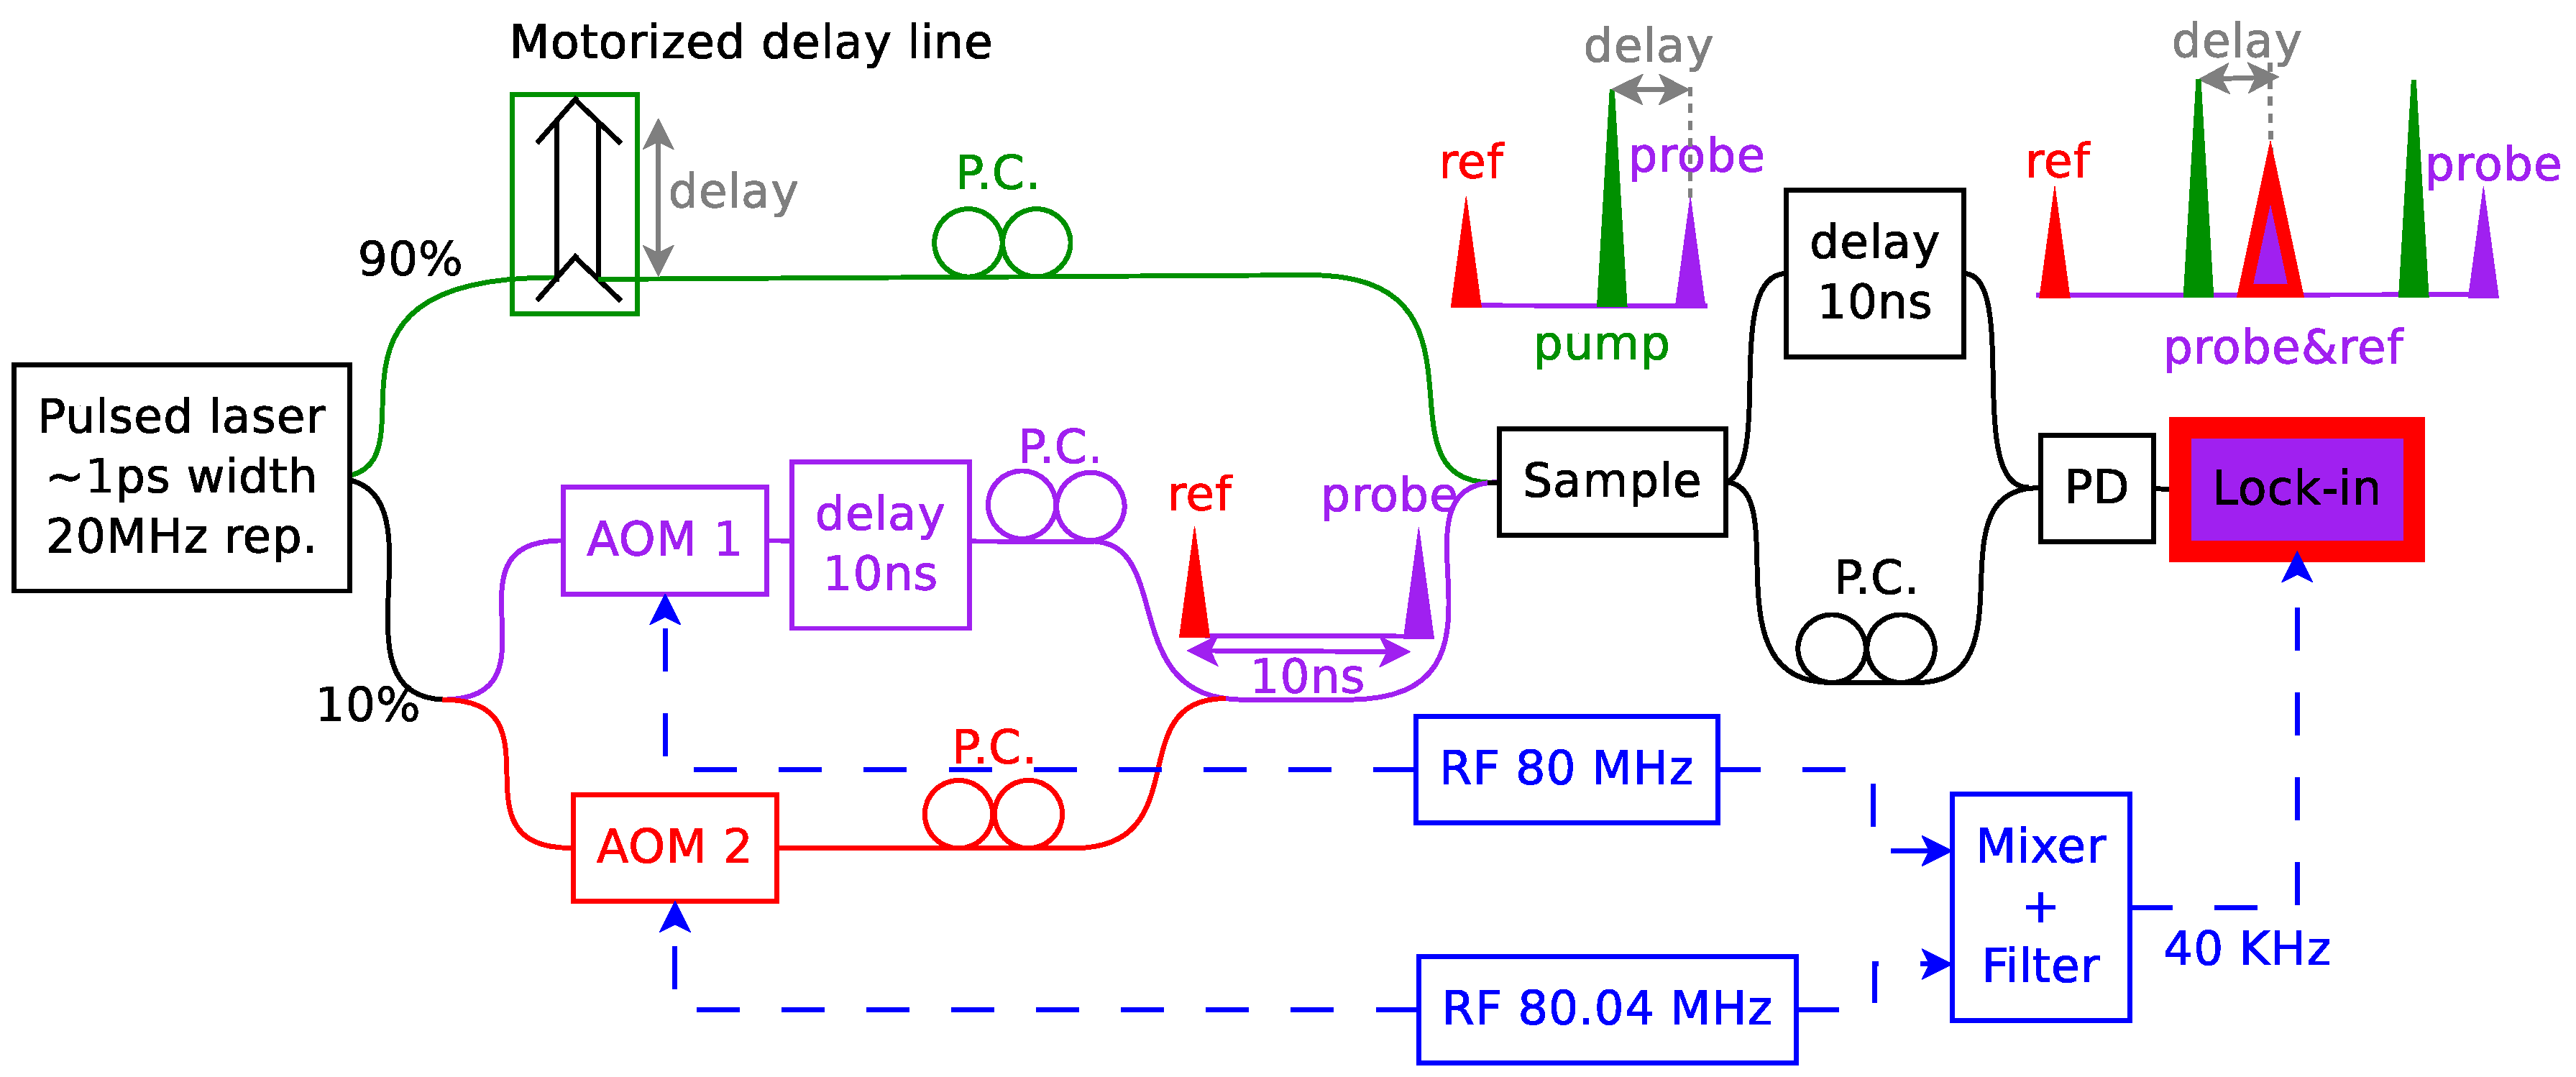
\includegraphics[width=0.95\textwidth]{timeResolved9}
                                         \caption{Time resolved characterization setup. PD: photodiode, PC: polarization controller, AOM: acousto-optic modulator.}
                                     \label{fig:setupTimeResTimeRes}
                                \end{figure}



In Fig.~\ref{fig:timeResolvesMeasurementsTimeRes} we observe the impact on transmission through the considered structures of both Kerr and carrier effect. The two effects produce opposite phase shifts because Kerr-effect increases the refractive index ($\Delta n > 0 $) and carriers decrease it ($ \Delta n < 0 $).  The dynamics  of these processes are also very different. During the pump pulse, an instantaneous phase change is due to Kerr effect; conversely after the pump pulse is gone, there is a phase response due to the carrier plasma effect (generally indicated as free-carrier dispersion - FCD) with positive sign that decays only on a much longer nanosecond time-scale. In order to investigate any degradation effects we exposed the waveguide to a high optical power for 1h and we did not observe any changes of the nonlinear optical performance.


\section{Time-resolved simulations}
In order to evaluate the propagation of pump and probe pulses in the optical waveguides and to fit Re$(\gamma)$ we applied the split-step simulation method to the nonlinear Schr\"{o}dinger equation (NLSE), considering the attenuation, dispersion, TPA, Kerr nonlinearity and the FCD effect.
Using this method the overall propagation-length is divided in a series of steps significantly smaller than both the pulse dispersive length and the nonlinear length ~\cite{Agrawal2001a,Lin2007}.
In the simulation program we inserted the experimentally measured waveguide losses, group velocity dispersion (measured using the technique reported in \cite{Mas2012}) and TPA coefficients obtained in section 3. Raman, pulse self-steepening, and higher-order dispersion terms terms have been neglected.
The effect of free carriers has been taken into account as in ~\cite{Lin2007}, where a carrier density averaged through the waveguide section is assigned to each simulation step. Carrier generation rate is governed by the TPA coefficient, while carrier decay time is assumed to be much longer than the pulse duration.
Finally the FCA and FCD coefficients dictate the effect of the carriers on the instantaneous absorption and refractive index of the waveguide respectively.
We have considered the FCA and FCD parameter definitions shown in Ref.~\cite{Lin2007}. In Table 1 we show all the parameters used in the simulation, except for the FCA coefficient, as from the experiment the effect of FCA was too weak to get a reliable estimation. By means of numerical simulations we obtain the envelope and the phase of the pump, probe and reference pulses at the waveguide output.
The output of the lock-in amplifier is the amplitude and the phase of the beatings produced by the heterodyne signal.
This magnitude is the Fourier component at 40~kHz of the sum of the reference and probe signals.
As the central frequencies of these two pulses differ in 40~kHz, this is equal to the overlap integral of their complex envelopes $E_{\mathrm{ref}}$ and $E_{\mathrm{probe}}$, obtaining:


                                                                \begin{equation}
                                                                        |T_{A}|e^{j\phi} =
                                                                        \frac{\int E_{\mathrm{ref}}(\tau) E^*_{\mathrm{probe}}(\tau) ~ \mathrm{d}\tau}
                                                                        {\int |E_{\mathrm{ref}}(\tau)|^2~\mathrm{d}\tau}
                                                                \end{equation}


 %\vspace*{-15pt}                                                                                                                          
                                                                
\begin{figure}[htb]
  \centering
  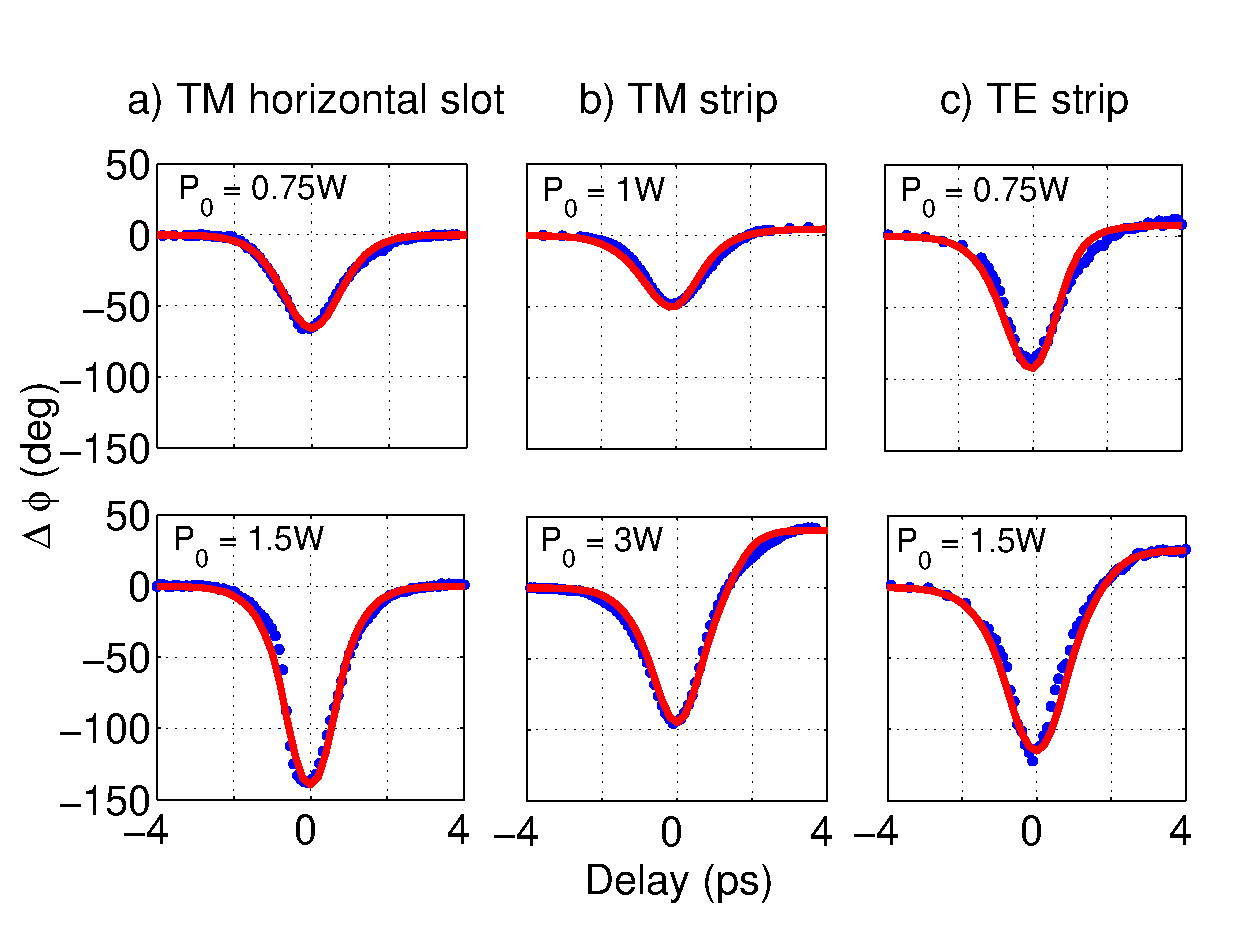
\includegraphics[width=0.77\textwidth]{measurements_v9}
  \caption{Time resolved measurements (blue dotted curves) and simulations (red continuous curves). Samples (a)TM-slot (0.75 and 1.5~W peak power) (b)TM-strip (1 and 3~W peak power) (c)TE-strip (0.75 and 1.5~W peak power).}
  \label{fig:timeResolvesMeasurementsTimeRes}
\end{figure}

where $T_A$ and $\phi$ are the amplitude and phase measured by the lock--in amplifier.
To evaluate Re$(\gamma)$ from the experimental data we performed numerical simulations (using a routine based on the split-step propagation method) in order to identify the Re$(\gamma)$ value yielding the best fit of the phase curve for each structure. In order to check for the results consistency we performed the experiments at two different power levels, obtaining two slightly different Re$(\gamma)$-values for each structure. In Table~\ref{tab:resultsArticleSlot} we report for each waveguide the average Re$(\gamma)$-value and its mean absolute deviation. 
The obtained results confirm that the slot-TM waveguide exhibits a higher nonlinear efficiency with respect to strip waveguides, that can be attributed to the high field confinement and to the interaction with silicon nanocrystals.


 \begin{table}[htb]
                        \centering
                        \caption{Extracted linear and nonlinear parameters from the experiment for the three samples: the horizontal slot, the  485$\times$220~nm TM strip and the  445$\times$220~nm TE strip waveguide. Dispersion values obtained with the technique shown in paper \cite{Mas2012}.}
                                \begin{tabular}{l|ccc}
                                        \hline
                                        Sample & TM slot & TM strip & TE strip\\\hline
                                        Coupling loss (dB) & 8 & 6 & 6\\
                                        Propagation loss (dB/cm) & 12 & 1.9 & 4.9\\
                                        $L_{eff}$ (mm) & 3.1 & 15.2 & 8.3\\
                                        Dispersion  (ps/(km$\cdot$nm))  & -1110 & -19800 & -1200\\
                                        $ Im(\gamma)~(\mathrm{W}\cdot \mathrm{m})^{-1} $          & -11.8 & -5.4 & -68.1\\
                                        $ Re(\gamma)~(\mathrm{W}\cdot \mathrm{m})^{-1} $          & 428$\pm$ 8 & 30 $\pm$ 3 & 235 $\pm$ 30\\
                                        $ FOM = \frac{1}{4\pi} \frac{Re(\gamma)}{|Im(\gamma)|} $  & 2.9 $\pm 0.06$ & 0.44 $\pm 0.05$ & 0.27$\pm 0.05$ \\
                                        effective FCD $ \frac{-\sigma_n}{ A_{eff} }~(10^{-15}~\mathrm{m}) $  & \textless 2 & 21 & 28 \\
                                        \hline
                                \end{tabular} 
\label{tab:resultsArticleSlot}
\end{table}



\section{Results and conclusion}
The first significant result is that phase measurements clearly show that the slot waveguide not only has a low TPA but also that free carriers have a negligible role.
This is clear from Fig. \ref{fig:timeResolvesMeasurementsTimeRes} where the phase-curve is only slightly affected by the free-carrier contribution. On the contrary the response of strip waveguides shows a long tail with $\Delta n <0$ for delay times longer than 1~ns.
This is confirmed by the FCD parameter, defined in~\cite{Lin2007} and shown in Table \ref{tab:resultsArticleSlot} (we have considered the effective FCD, which is normalized with the effective area, making it a device parameter like $\gamma$, rather than a material parameter).
This feature considerably reduces the undesired patterning effects when modulating a real bit pattern. On the other hand, the figure of merit (FOM) given by the ratio between Kerr effect and TPA is also significantly higher in the slot waveguide than in the strip waveguides: $2.9\pm 0.06$ for the slot, $0.44 \pm 0.05$ and $0.27 \pm 0.05$ respectively for the TM and TE strip waveguides, as reported in Table~\ref{tab:resultsArticleSlot}.
It is worth underlining that the FOM obtained by the TE and TM waveguides well agree with the values reported by state of the art all-silicon waveguides~\cite{Koos2007a}.


All these findings can be explained by the fact that in the slot waveguide, a considerable amount of energy travels through the slot layer, which provides a very efficient Kerr effect~\cite{Trita2011} and a weak TPA.
Nevertheless we note that the optical performance of such waveguides depends on their structure as well as on the conditions of deposition of both the silicon nanocrystals layer and the Si top layer. It is interesting to highlight that considering different waveguide diameters it is possible, according to~\cite{Rukhlenko2012}, to greatly reduce the effective area and increase the amount of energy traveling through the slot region in comparison to the current waveguide design.
That would allow increasing the beam intensity in the structure thus boosting the nonlinear effects, provided that the increase of coupling losses do not completely overtake the advantages given by the optimized structure.
On the other hand, comparing the TM and TE strips, we find that the TM has a higher FOM but lower $\gamma$ than the TE.
This is expected, as the TM mode is weakly confined in the vertical direction, therefore more energy travels through the cladding, which has lower Kerr coefficient and negligible TPA.
Finally, the performance of the device is similar to the one shown in Ref.~\cite{Vallaitis2008} for a polymer-filled vertical slot; however, our system, being made of inorganic materials and only requiring CMOS processes, is expected to provide more robust and stable devices with less temperature constraints. 

In conclusion, ultrafast nonlinear measurements show that silicon-nanocrystal-based horizontal slot waveguides show weaker carrier effects and better FOM than Si strip waveguides.
This makes the slot structure better suited for CMOS-compatible high-speed all-optical processing than simple Si strip waveguides.

\section*{Acknowledgments}
We acknowledge EU-project PHOLOGIC (FP6-IST-NMP-017158), Spanish Ministry of Science and Innovation SINADEC (TEC2008-06333) and PROMETEO/2010/087 NANOFOTONICA projects and Universidad Polit\'ecnica de Valencia for PAID2011/1914 and J. Matres' doctoral grant.


%\bibliographystyle{osajnl}
%\bibliography{library}
\bibliographystyle{unsrt}
\begin{thebibliography}{10}
\newcommand{\enquote}[1]{``#1''}

\bibitem{Almeida2004b}
V.~R. Almeida, C.~A. Barrios, R.~R. Panepucci, and M.~Lipson,
  \enquote{{All-optical control of light on a silicon chip.}} Nature
  \textbf{431}, 1081--1084 (2004).

\bibitem{Lee2009}
B.~G. Lee, A.~Biberman, A.~C. Turner-Foster, M.~A. Foster, M.~Lipson, A.~L.
  Gaeta, and K.~Bergman, \enquote{{Demonstration of broadband wavelength
  conversion at 40 Gb/s in silicon waveguides},} IEEE Photon. Technol. Lett. \textbf{21}, 182--184 (2009).

\bibitem{Driscoll2010}
J.~B. Driscoll, W.~Astar, X.~L.~X. Liu, J.~I. Dadap, W.~M.~J. Green, Y.~A.
  Vlasov, G.~M. Carter, and R.~M. Osgood, \enquote{{All-optical wavelength
  conversion of 10 Gb/s RZ-OOK data in a silicon nanowire via cross-phase
  modulation: Experiment and theoretical investigation},} IEEE J. Sel. Top. Quantum Electron \textbf{16}, 1448--1459 (2010).

\bibitem{Koos2009}
C.~Koos, P.~Vorreau, T.~Vallaitis, P.~Dumon, W.~Bogaerts, R.~Baets,
  B.~Esembeson, I.~Biaggio, T.~Michinobu, F.~Diederich, W.~Freude, and
  J.~Leuthold, \enquote{{All-optical high-speed signal processing with silicon
  – organic hybrid slot waveguides},} Nature Photonics \textbf{3}, 1--4
  (2009).

\bibitem{Astar2010}
W.~Astar, J.~B. Driscoll, X.~L.~X. Liu, J.~I. Dadap, W.~M.~J. Green, Y.~A.
  Vlasov, G.~M. Carter, and R.~M. Osgood, \enquote{{All-Optical Format
  Conversion of NRZ-OOK to RZ-OOK in a Silicon Nanowire Utilizing Either XPM or
  FWM and Resulting in a Receiver Sensitivity Gain of 2.5 dB},} IEEE J. Sel. Top. Quantum Electron \textbf{16}, 234--249 (2010).

\bibitem{Foster2008}
M.~A. Foster, A.~C. Turner, M.~Lipson, and A.~L. Gaeta, \enquote{{Nonlinear
  optics in photonic nanowires.}} Opt. Express \textbf{16}, 1300--1320
  (2008).

\bibitem{Osgood2009}
R.~M. Osgood, Jr., N.~C. Panoiu, J.~I. Dadap, X.~Liu, X.~Chen, I.-W. Hsieh,
  E.~Dulkeith, W.~M. Green, and Y.~A. Vlasov, \enquote{{Engineering
  nonlinearities in nanoscale optical systems: physics and applications in
  dispersion-engineered silicon nanophotonic wires},} Adv. Opt. Photon. \textbf{1}, 162 (2009).

\bibitem{Almeida2004}
V.~R. Almeida, Q.~Xu, C.~A. Barrios, and M.~Lipson, \enquote{{Guiding and
  confining light in void nanostructure.}} Opt. Lett. \textbf{29}, 1209--1211
  (2004).

\bibitem{Sanchis2007}
P.~Sanchis, J.~Blasco, A.~Martinez, and J.~Marti, \enquote{{Design of
  Silicon-Based Slot Waveguide Configurations for Optimum Nonlinear
  Performance},} J. Lightwave Technol. \textbf{25}, 1298--1305
  (2007).

\bibitem{Koos2007a}
C.~Koos, L.~Jacome, C.~Poulton, J.~Leuthold, and W.~Freude, \enquote{{Nonlinear
  silicon-on-insulator waveguides for all-optical signal processing.}} Opt. Express \textbf{15}, 5976--5990 (2007).

\bibitem{Zhang2010}
L.~Zhang, Y.~Yue, Y.~Xiao-Li, J.~Wang, R.~G. Beausoleil, and A.~E. Willner,
  \enquote{{Flat and low dispersion in highly nonlinear slot waveguides.}}
  Opt. Express \textbf{18}, 13187--13193 (2010).

\bibitem{Rukhlenko2012}
I.~D. Rukhlenko, M.~Premaratne, and G.~P. Agrawal, \enquote{{Effective mode
  area and its optimization in silicon-nanocrystal waveguides.}} Opt. Lett.
  \textbf{37}, 2295--2297 (2012).

\bibitem{Spano2009}
R.~Spano, N.~Daldosso, M.~Cazzanelli, L.~Ferraioli, L.~Tartara, J.~Yu,
  V.~Degiorgio, E.~Giordana, J.~M. Fedeli, and L.~Pavesi, \enquote{{Bound
  electronic and free carrier nonlinearities in Silicon nanocrystals at
  1550nm.}} Opt. Express \textbf{17}, 3941--3950 (2009).

\bibitem{Martinez2010a}
A.~Mart\'{\i}nez, J.~Blasco, P.~Sanchis, J.~V. Gal\'{a}n,
  J.~Garc\'{\i}a-Rup\'{e}rez, E.~Jordana, P.~Gautier, Y.~Lebour,
  S.~Hern\'{a}ndez, R.~Guider, N.~Daldosso, B.~Garrido, J.~M. Fedeli,
  L.~Pavesi, J.~Mart\'{\i}, and R.~Spano, \enquote{{Ultrafast all-optical
  switching in a silicon-nanocrystal-based silicon slot waveguide at telecom
  wavelengths.}} Nano Lett. \textbf{10}, 1506--1511 (2010).

\bibitem{Oton2010}
C.~J. Oton, J.~Matres, A.~Martinez, P.~Sanchis, J.~P. Colonna, C.~Ratin, J.~M.
  Fedeli, and J.~Marti, \enquote{{Ultrafast all-optical logic gates with
  silicon nanocrystal-based slot waveguides},} in Proc. of 7th IEEE Int. Conf. on Group IV Photonics, 171–-173 (IEEE, 2010).

\bibitem{Trita2011}
A.~Trita, C.~Lacava, P.~Minzioni, J.-P. Colonna, P.~Gautier, J.-M. Fedeli, and
  I.~Cristiani, \enquote{{Ultra-high four wave mixing efficiency in slot
  waveguides with silicon nanocrystals},} Appl. Phys. Lett. \textbf{99},
  191105 (2011).

\bibitem{Garcia2004}
C.~Garcia, B.~Garrido, P.~Pellegrino, J.~R. Morante, M.~Melchiorri,
  N.~Daldosso, L.~Pavesi, E.~Scheid, and G.~Sarrabayrouse, \enquote{{Low loss
  Silica waveguides containing Si nanocrystals},} in \enquote{New Materials for
  Microphotonics, Ed. J. H. Shin, M. Brongersma, C. Buchal, F. Priolo, MRS
  Proceedings,}  (2004),\textbf{817}, L4.1--L4.6.

\bibitem{Jordana2007}
E.~Jordana, J.-M. Fedeli, P.~Lyan, J.~P. Colonna, P.~E. Gautier, N.~Daldosso,
  L.~Pavesi, Y.~Lebour, P.~Pellegrino, B.~Garrido, J.~Blasco, F.~Cuesta-Soto,
  and P.~Sanchis, \enquote{{Deep-UV Lithography Fabrication of Slot Waveguides
  and Sandwiched Waveguides for Nonlinear Applications},} in Proc. of 4th IEEE Int. Conf. on Group IV Photonics, 1–-3 (IEEE, 2007).
  
\bibitem{Mizrahi}
V.~Mizrahi, K.~W. Delong, G.~I. Stegeman, M.~A. Saifi, and M.~J. Andrejco,
  \enquote{{Two-photon absorption as a limitation to all-optical switching.}}
  Opt. Letters \textbf{14}, 1140--1142 (1989).

\bibitem{Vallaitis2009}
T.~Vallaitis, S.~Bogatscher, L.~Alloatti, P.~Dumon, R.~Baets, M.~L. Scimeca,
  I.~Biaggio, F.~Diederich, C.~Koos, W.~Freude, and J.~Leuthold,
  \enquote{{Optical properties of highly nonlinear silicon-organic hybrid (SOH)
  waveguide geometries.}} Opt. Express \textbf{17}, 17357--17368 (2009).
  
\bibitem{Buuren98}
T.~van Buuren, L.~Dinh, L.~Chase, W.~Siekhaus, and L.~Terminello, \enquote{{Changes in the Electronic Properties of Si Nanocrystals as a Function of Particle Size}}. Phys. Rev. Lett., \textbf{80}, 3803–-3806 (1998).

\bibitem{Bassani}
Z.~Gaburro, N.~Daldosso, L.~Pavesi, \enquote{Porous Silicon}, Encyclopedia of Condensed Matter Physics edited by F.~ Bassani, J.~Liedl and P.~Wyder (Elsevier Academic Press, 2005)

\bibitem{Daldosso2009}
N.~Daldosso and L.~Pavesi, \enquote{Nanosilicon photonics}. Laser Photonics Rev., \textbf{3}, 508–-534 (2009).

\bibitem{Vallaitis2008}
T.~Vallaitis, C.~Koos, R.~Bonk, W.~Freude, M.~Laemmlin, C.~Meuer, D.~Bimberg,
  and J.~Leuthold, \enquote{{Slow and fast dynamics of gain and phase in a
  quantum dot semiconductor optical amplifier.}} Opt. Express \textbf{16},
  170--178 (2008).

\bibitem{Agrawal2001a}
G.~P. Agrawal, \emph{{Nonlinear Fiber Optics}}, (Academic Press, 2001).

\bibitem{Lin2007}
Q.~Lin, O.~J. Painter, and G.~P. Agrawal, \enquote{{Nonlinear optical phenomena
  in silicon waveguides: modeling and applications.}} Opt. Express
  \textbf{15}, 16604--16644 (2007).

\bibitem{Mas2012}
S.~Mas, J.~Matres, J.~Marti, and C.~J. Oton, \enquote{{Accurate chromatic
  dispersion characterization of photonic integrated circuits},} IEEE Photon. J. \textbf{4}, 825--831 (2012).

\end{thebibliography}

\chapter{Paper:~High nonlinear figure-of-merit amorphous silicon}
\label{ch:articleFigureOfMerit}
In this work we propose using amorphous silicon for all-optical switching. Its higher band-gap, lower carrier generation and carrier lifetime makes amorphous silicon, an ideal candidate for all-optical switching.
Using amorphous silicon we measured a very high nonlinear figure of merit.
My contribution to the paper was the following: I made the experimental measurements, analyzed the data and drafted the paper. For the simulations, I used a split-step Fourier method which was coded by G. Ballesteros. The paper was published in Optics Express, and the reference is the following:

\vspace{1.5cm}

J Matres, G C Ballesteros, P. Gautier, J M Fedeli, J Marti and C J Oton. High nonlinear figure-of-merit amorphous silicon waveguides. Opt. Express, 21(4):1164–1170, 2013

\newpage
\begin{center}
\section*{High nonlinear figure-of-merit amorphous silicon waveguides}
{J. Matres,$^{*,1}$ G. C. Ballesteros,$^1$ P. Gautier,$^2$ J-M F\'ed\'eli,$^2$  J. Mart\'i,$^1$ and C. J. Oton,$^{1,3}$} 
\end{center}

\noindent
\textit{$^1$ Nanophotonics Technology Center, Universidad Polit\'ecnica de Valencia, Camino de Vera s/n, 46022, Valencia, Spain\\
$^2$CEA LETI, Minatec Campus, Grenoble 38054, France\\
$^3$Current address: Scuola Superiore Sant'Anna, Via G. Moruzzi 1, 56124, Pisa, Italy}

\begin{center}
{$^*$joamatab@ntc.upv.es}
\end{center}


\textbf{Abstract} \\
\noindent
The nonlinear response of amorphous silicon waveguides is reported and compared to silicon-on-insulator (SOI) samples.
The real part of the nonlinear coefficient $\gamma$ is measured by four-wave-mixing and the imaginary part of $\gamma$ is characterized by measuring the nonlinear loss at different peak powers.
The combination of both results yields a two-photon-absorption figure of merit of 4.9, which is more than 7 times higher than for the SOI samples.
Time-resolved measurements and simulations confirm the measured nonlinear coefficient $\gamma$ and show the absence of slow free-carrier effects versus ns free-carrier lifetimes in the SOI samples.

\begin{center}
{(190.0190) Nonlinear optics; (130.0130) Integrated optics; (190.4380) Nonlinear optics, four-wave mixing; (160.4330) Nonlinear optical materials.}
\end{center}

\section{Introduction}
Silicon photonics technology is becoming increasingly competitive with respect to alternative platforms, in particular because devices can be mass-produced using CMOS technology at a very low cost per unit. Implementing nonlinear functions in silicon photonics, e.g. all-optical switching or routing, has attracted significant interest since they allow much higher speeds compared to electrically-controlled switches. Many different nonlinear devices have been reported in the last years, such as all-optical modulators,~\cite{Almeida2004b} wavelength converters,~\cite{Lee2009} and parametric amplifiers~\cite{Kuyken2011a}. Moreover, all of them can be easily integrated to generate more complex devices within a small area thanks to the high refractive index of silicon.


The main drawback of silicon for realizing nonlinear functionalities at telecom wavelength (around 1550~nm) is two-photon absorption (TPA) effect, not only because of the lost photons in the process but also because the generated carriers subsequently produce usually undesired free carrier absorption (FCA) and dispersion (FCD).
As the Kerr response of the device is determined by $Re\{\gamma\}$ and TPA is given by $Im\{\gamma\}$, a TPA figure-of-merit (FOM) can be defined as $Re\{\gamma\}/(4\pi |Im\{\gamma\}|)$  \cite{Mizrahi1989}. This provides a useful dimensionless measurement of the suitability of the material for nonlinear switching, where it is usually considered as suitable if this number is greater than two.
This is the reason why a material different from crystalline silicon is needed.
Amorphous silicon (a-Si) has been demonstrated to have a high nonlinear coefficient \cite{Narayanan2010} and low TPA thanks to its wider band-gap \cite{OLeary1997}.
Furthermore, it is a material that can be easily grown in CMOS compatible processes.
As a-Si does not need high annealing temperatures, it is a good candidate for all-optical interconnects in between different chips and it could be grown on a top layer not affecting circuits already integrated on the chip.



On the other hand, a-Si does not always have the same optical properties, as its composition (\emph{i.e.} hydrogen content) or atomic arrangement can vary depending on the fabrication conditions.
In Ref.~\cite{Narayanan2010} a $Re\{\gamma\} \simeq 2000~(\mathrm{W}\cdot\mathrm{m})^{-1}$ nonlinear coefficient was presented, but TPA was also high, leading to a figure of merit of 0.66. However, in Ref.~\cite{Kuyken2011}, a FOM larger than two was reported. In that work, a degradation of the material within minutes of light exposure was also reported.
Here, we report the characterization of the real and imaginary parts of $\gamma$ of a-Si samples with a FOM of 4.9 and no observed material degradation.


\section{Fabrication}
Starting with Si bulk wafers oxidized with 3~$\mu \mathrm{m}$ thickness, a hydrogenated amorphous silicon layer of 253~nm was deposited by Plasma-enhanced chemical vapor deposition (PECVD) at 350~$^\circ$. Waveguides were patterned using DUV lithography and HBr Reactive-ion etching, then covered with 1.5~$\mu \mathrm{m}$ m thick silica. Waveguides of 475~nm width and 20~mm length were fabricated and light was coupled horizontally using lensed fibers.

On the other hand, SOI waveguides were also fabricated for comparison. These were processed from SOI wafers with 220~nm Si thickness, patterned with deep-UV lithography and covered with silica after the etching process. Their dimensions were  445$\times$220~nm  for transverse-electric (TE) polarization and 485$\times$220~nm for transverse-magnetic (TM) polarization. Total length was 25~mm and light was coupled through grating couplers.

Figure \ref{fig:sem} shows scanning electron microscopy (SEM) micrographs of the facets. Propagation and coupling loss were measured by characterizing waveguides of different lengths (results are shown in Table \ref{tab:resultsFOMpaper}). 


%Then using DUV lithography and HBr RIE etching waveguides were formed and covered with $1.5\mu m$ thick silica.

\begin{figure}[htb]
    \centering
    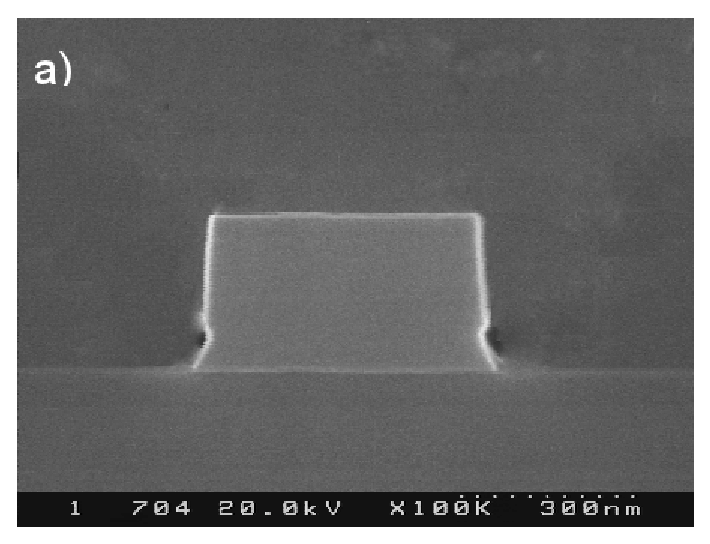
\includegraphics[width=0.325\textwidth]{p13_4}
    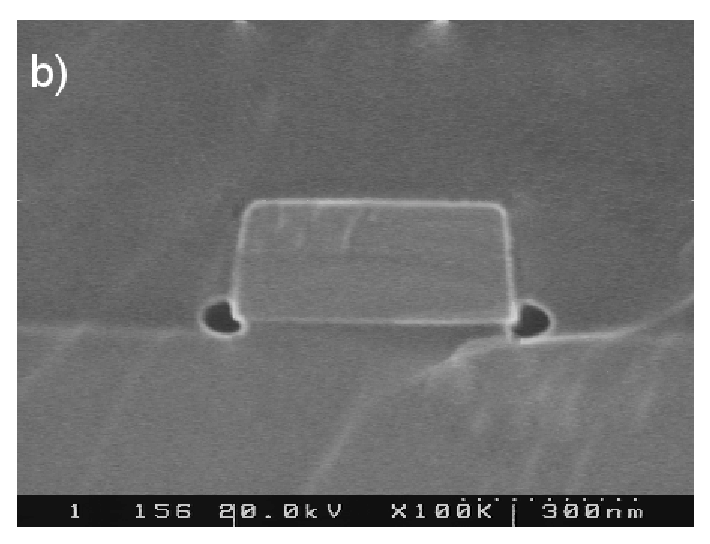
\includegraphics[width=0.325\textwidth]{semTM_4}
    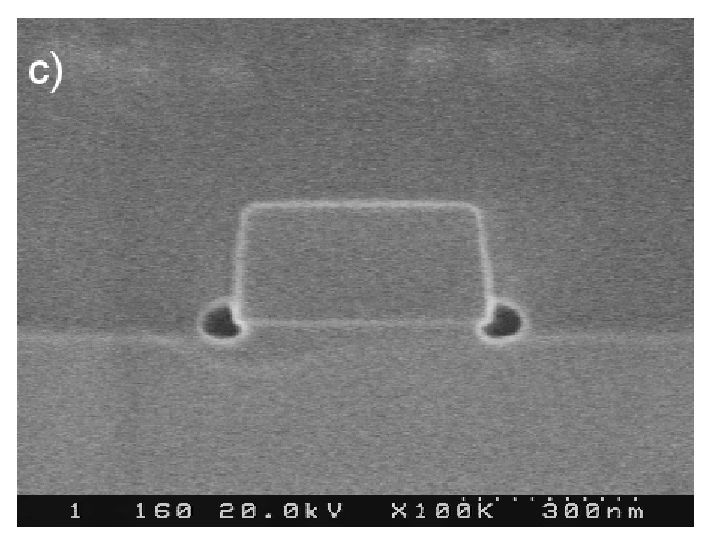
\includegraphics[width=0.325\textwidth]{semTE_2}
    \caption{SEM images of the amorphous silicon (a), TM SOI (b) and TE SOI (c). Air bubbles visible in the SOI samples were generated during facet preparation with HF to increase SEM contrast.}
    \label{fig:sem}
\end{figure}


%%%%%%%%%%%%%%%%%%%%%%%%%%
%%%%%%     Experiments      %%%%%%%%%%%
%%%%%%%%%%%%%%%%%%%%%%%%%%

\section{Four-wave-mixing: Re$\{ \gamma \}$}
Two continuous wave (cw) lasers were coupled to the waveguides, a pump beam with power $P_P(0)$ and a weaker signal beam with power $P_S(0)$, generating an idler signal at the waveguide output $P_i(L)$.
We measured the conversion efficiency as a function of the wavelength separation between pump and signal by using an optical spectrum analyzer (OSA) as shown in Fig.~\ref{fig:fwmOSA}.
Assuming that at these power levels (below 15~dBm) TPA is negligible, we can use Eq.~(\ref{eq:FWM}) as in Ref.~\cite{Vallaitis2009}.

%(Fig.~\ref{fig:fwmSetup}

%\begin{equation}
%       \eta ^2=\frac{\alpha_0^2}{\alpha_0^2+\Delta \beta^2}\left[ 1+ 4e^{-\alpha_0L}\frac{sin^2(L\Delta\beta/2)}{(1-e^{-\alpha_0L})^2} \right]
%\end{equation}

%where $ \Delta\beta $ for a detuning $ \Delta\lambda = \lambda_p-\lambda_s$ is given by:

%\begin{equation}
%       \Delta \beta=\frac{2\pi cD_2}{\lambda_p^2}\Delta\lambda^2
%\end{equation}



\begin{equation}
        P_i(L)=e^{-\alpha_0L}(\eta Re\{\gamma\}P_P(0)L_{eff})^2 P_s(0)
\label{eq:FWM}
\end{equation}


where $\alpha_0$ is the propagation loss, $L$ the waveguide total length, and $ L_{eff} $ the effective length, defined as $[ 1-\mathrm{exp}(-\alpha_0 L)] / \alpha_0 $

%where $\alpha_0$ is the propagation loss, $L$ the waveguide total length, and $ L_{eff} $ the effective waveguide length, which is defined as:
%\begin{equation}
        %L_{eff}=\frac{1-e^{-\alpha_0L}}{\alpha_0}
%\end{equation}

Finally, the conversion efficiency $\eta$ is given by \cite{Kung2003,Systems2004}:

\begin{equation}
        \eta ^2=\frac{\alpha_0^2}{\alpha_0^2+\Delta \beta^2}\left( 1+ 4e^{-\alpha_0L}\frac{sin^2(L\Delta\beta/2)}{1-e^{-\alpha_0L}} \right)
\end{equation}

where the phase mismatch for a detuning $ \Delta\lambda = \lambda_p-\lambda_s$ is

\begin{equation}
        \Delta \beta=\frac{2\pi cD_\lambda}{\lambda_p^2}\Delta\lambda^2
\end{equation}

where $D_\lambda$ is the chromatic dispersion parameter. One can relate the idler output to the signal output by rearranging Eq.~(\ref{eq:FWM}) obtaining

\begin{equation}
        \frac{P_i(L)}{P_s(L)}=(\eta Re\{\gamma\}P_P(0)L_{eff})^2 
\label{eq:ratio}
\end{equation}

which is the equation used for the calculation of $Re\{\gamma\}$ and dispersion $D_\lambda$ from the OSA spectra. Results are shown in Fig.~\ref{fig:fwmBw} and parameters of the fit are shown in Table~\ref{tab:resultsFOMpaper}.
The sign of the dispersion cannot be extracted from this method, but knowing the waveguide geometry, we calculated the dispersion of the waveguides using Finite Elements simulations.
We found a good fit with the numeric results shown in Table~\ref{tab:resultsFOMpaper} within a 10\% error, so this gave us the sign of dispersion. Dispersion of the SOI samples was also experimentally characterized with an interferometric setup obtaining a good agreement too \cite{Mas2012}.


%Moreover fitting the conversion bandwidth to equation~\ref{eq:ratio}
%\begin{figure}[htb]
 %  \centering
  %  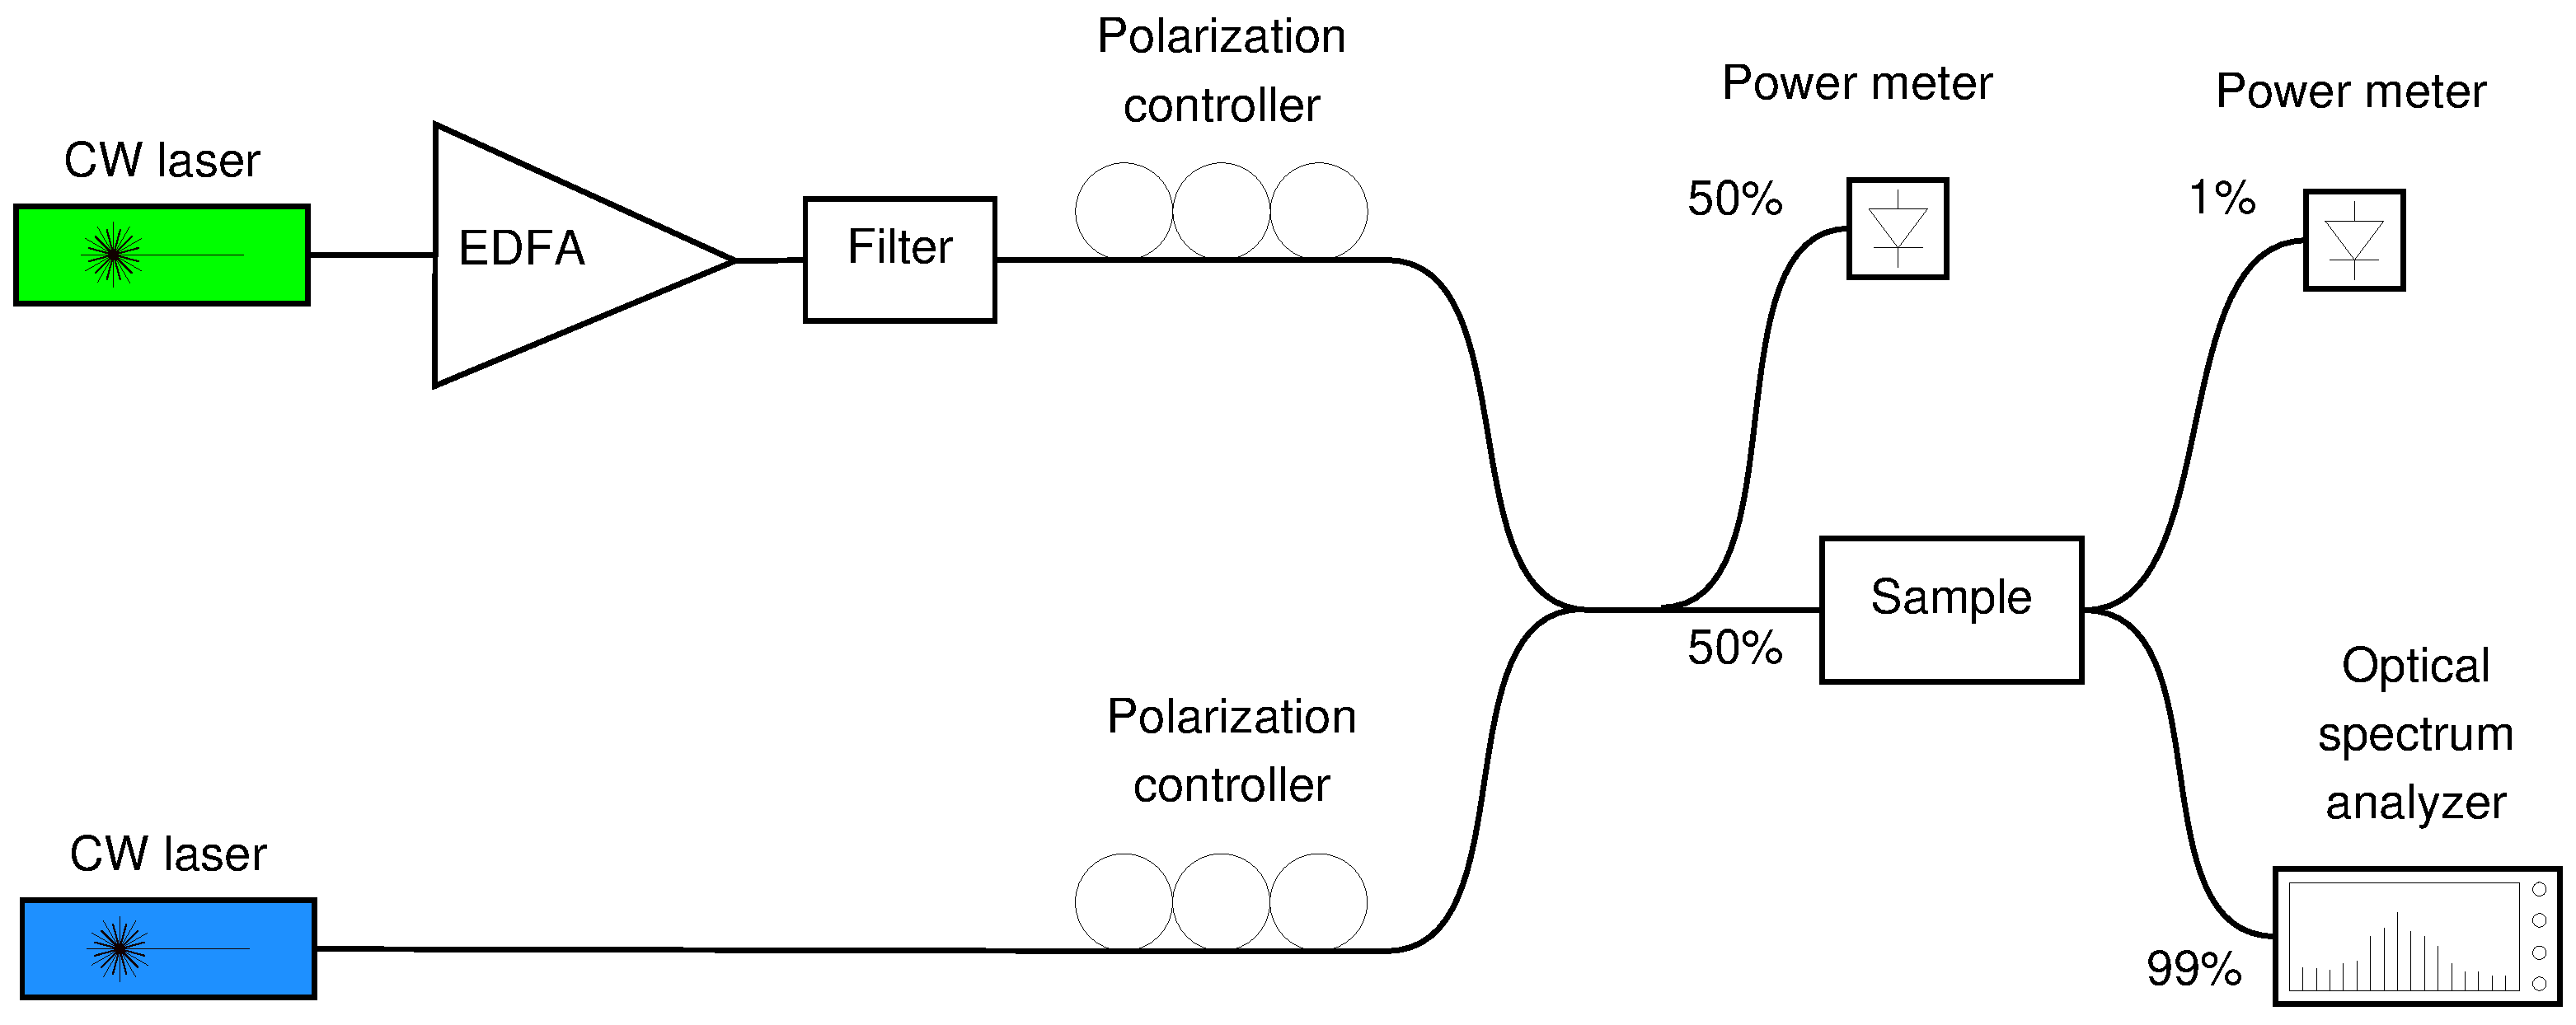
\includegraphics[width=1.00\textwidth]{fwmOneEdfa}s
   % \caption{Four Wave Mixing characterization setup.}
    %\label{fig:fwmSetup}
     %\end{figure}


\begin{figure}[htb]
    \centering
    \includegraphics[width=0.45\textwidth]{Power_dBm_fwm_convEffMax_29p5dB}
    \caption{With 13~dBm pump power in waveguide a signal to idler conversion efficiency of -29.5~dB was measured in the FWM experiment.}
    \label{fig:fwmOSA}
\end{figure}
%Different signals in the FWM experiment. An idler with -29.5dB conversion efficiency was measure for 13dBm pump power in waveguide

\begin{figure}[htb]
    \centering
    \includegraphics[width=0.32\textwidth]{fwm_bandwidth_P13_TM20mm_15dBmPump_6dBcm_332Wm_6474psKmnm_big_1pointMore}
    \includegraphics[width=0.32\textwidth]{fwm_bandwidth_V740_C11_TM25mm_20dBm_pump_1p67_46p81_19860psKmnm_big}
    \includegraphics[width=0.32\textwidth]{fwm_BW_V740C11_TE25mm_15dBmPump_3p8dBcm_361Wm_-1322psKmnm_big}
    \caption{Four wave mixing conversion efficiency bandwidth. Pump power: 7.5~dBm (sample a), 14~dBm (sample b), 9~dBm (sample c). Dots are experimental points and the solid line is the fit to Eq.~(\ref{eq:ratio}).}
    \label{fig:fwmBw}
\end{figure}

We also show in Fig.~\ref{fig:fwmDifferentPump} the conversion efficiency for different input pump powers, where a slope very close to 2 was observed in all cases, confirming that the parametric conversion depends quadratically on the pump power.

\begin{figure}[htb]
    \centering
    \includegraphics[width=0.32\textwidth]{fwm_differentPumps_aSitm20mm}
    \includegraphics[width=0.32\textwidth]{fwm_differentPumps_tm}
    \includegraphics[width=0.32\textwidth]{fwm_differentPumps_te}
    \caption{Four wave conversion efficiency versus pump power. Dots: experimental points, solid line: linear fit. The slope of the linear fit in dB represents the power of the conversion efficiency versus pump power, which is close to 2 in all cases.}
    \label{fig:fwmDifferentPump}
\end{figure}






\section{Nonlinear loss measurements: Im\{$ \gamma $\}}
\label{sec:imGamma}
Two-photon absorption is a well-known process in silicon waveguides.
In a waveguide, we can consider it as the imaginary part of the gamma coefficient of the waveguide by using this differential equation:

\begin{equation}
 \frac{dP}{dz} = -\alpha_0 P(z) - 2|Im(\gamma)| P(z)^2 
\label{eq:differentialTPA}
\end{equation}

where P is the signal power through the waveguide, $\alpha$ is the linear loss of the waveguide, and $Im(\gamma)$ is the imaginary part of the $\gamma$ coefficient (we use the absolute value because we want to stress its loss character in the equation with a negative sign). 

The solution of the differential equation shown in Eq.~(\ref{eq:differentialTPA}) after a distance $L$ is given by:

\begin{equation}
 P(L) = \frac{e^{-\alpha_0 L}}{1+2|Im(\gamma)| L_{eff} P_0} P_0
\end{equation}

where $P_0$ is the input power in the waveguide. Therefore the ratio between the transmission at low power ($T_{LP} = e^{-\alpha_0 L} $) and the transmission at high power ($T_{HP} = P(L)/P_0 $) represents only the nonlinear loss $T_{NL}^{-1}$:

\begin{equation}
 T_{NL}^{-1} = \frac{T_{LP}}{T_{HP}} = 1+2|Im(\gamma)| L_{eff} P_0
\label{eq:transmissionLinear}
\end{equation}

which is a linear function on $P_0$.
The slope of the curve can give us the two-photon absorption coefficient of our waveguide as in \cite{Vallaitis2009}.
However, this equation is only valid for instantaneous transmission values.
When a pulsed signal is sent, and the transmission is averaged over time, the measured transmission would be the integral of the output, which we can define as:

%If one sends a pulsed signal, the equation is still correct for every instantaneous moment, but not correct for the overall transmission energy of the pulse.
%If one defines the energy transmission of a pulse $ \tilde{T} $ as the amount read by a power meter, one has to integrate the power along the whole pulse duration:

\begin{equation}
 \tilde{T}  = \frac{\int P(t,L)dt}{\int P_0(t)dt}
\end{equation}

where $\tilde{T}$ represent the averaged transmission of a pulsed signal with an input shape given by $P_0(t)$. With this definition, the ratio with the transmission at low power would be given by:


%\begin{equation}
 %\tilde{T} (L)^{-1} = \frac{\int P_0(t)dt}{\int P(t,L)dt} = \frac{\int P_0(t)dt} {e^{-\alpha L} \int \frac{P_0(t)}{1+2|Im(\gamma)| L_{eff} P_0(t)} dt}
%\end{equation}

\begin{equation}
\tilde{T}_{NL}^{-1} = \frac{\tilde{T}_{LP}}{\tilde{T}_{HP}} = \frac{\int P_0(t)dt}{\int \frac{P_0(t)}{1+2|Im(\gamma)| L_{eff} P_0(t)} dt}
\label{eq:transmissionIntegral}
\end{equation}


which depends on the actual pulse shape $P_{0}(t)$ that is introduced. If the pulsed signal has a rectangular shape, one can use Eq.~(\ref{eq:transmissionLinear}), but if the shape is different, the integral in Eq.~(\ref{eq:transmissionIntegral}) must be solved, as the result differs significantly.
The reason for this variation is the fact that the flanks of the pulse are not affected as hardly by TPA as the peak. Therefore, the overall energy transmission is higher than for the case of cw excitation.
For the particular case of a $sech^2$ shape, which corresponds to the output of our laser, the result of  Eq.~(\ref{eq:transmissionIntegral}) is given by:

% One can calculate analytically how much this transmission is for different typical pulse shapes.

%We assume a hyperbolic secant pulse, typical for solitons, which is the shape of our femtosecond fiber laser $  P_0(t) = P_{0 peak}~\mathrm{sech}^2 (\frac{t}{\tau}) $. Solving Eq.~(\ref{eq:transmissionIntegral}) for the hyperbolic secant is not trivial. After some algebraic manipulation and using some properties of inverse hyperbolic trigonometric functions, one can extract the analytical result, which is:<

%\begin{equation}
% P_0(t) = P_{0 peak}~sech^2 \frac{t}{\tau}
%\end{equation}



\begin{equation}
\tilde{T}_{NL}^{-1} = \frac{\tilde{T}_{LP}}{\tilde{T}_{HP}} \bigg|_{sech^2~shape}  = \frac{\sqrt{\delta}\sqrt{\delta + 1}}{\ln(\sqrt{\delta}+\sqrt{\delta+1})} ~~\mathrm{where}~~  \delta = 2|Im(\gamma)| L_{eff} P_{0 peak}
\label{eq:transmissionHypSecant}
\end{equation}

%for $ \delta = 2|Im(\gamma)| L_{eff} P_{0 peak} $

%\begin{figure}[htb]
 %   \centering
  %  \includegraphics[width=1.0\textwidth]{imGammaFit}
   % \caption{Absorption characterization setup.}
    %\label{fig:setupImGamma}
%\end{figure}

We measured this parameter with a power meter using a picosecond laser at a wavelength of 1539~nm and a variable attenuator.
The results are shown in Fig.~\ref{fig:imGammaSamples}, where the curves were fitted to Eq.~(\ref{eq:transmissionHypSecant}) in order to extract the $Im(\gamma)$ parameter shown in Table~\ref{tab:resultsFOMpaper}.


%We measured the nonlinear loss with a power meter using a picosecond laser at a wavelength of 1539~nm and a variable attenuator. The results are shown in Fig.~\ref{fig:imGammaSamples}, where the curves were fitted to Eq.~\ref{eq:transmissionHypSecant} in order to extract the parameter $Im(\gamma)$ (see Table~\ref{tab:resultsFOMpaper}).

%In order to extract the $Im(\gamma)$ parameter, we measured the transmission for different peak powers using a picosecond laser at a wavelength of 1539~nm and a variable attenuator. The results substracting the linear loss (Fig.~\ref{fig:imGammaSamples}) were fitted to Eq.~\ref{eq:transmissionHypSecant} and shown in Table~\ref{tab:resultsFOMpaper}.


\begin{figure}[htb]
    \centering
    \includegraphics[width=1.0\textwidth]{imGamma_aSi_TM_TE}
      \caption{Transmission versus waveguide peak power (note the difference in the y-scale among the three plots). Solid line shows the fit for $ sech^2 $ pulses using Eq.~(\ref{eq:transmissionHypSecant}).}
    \label{fig:imGammaSamples}
\end{figure}



\section{Time-resolved measurements and simulations}
We characterize the samples with a time-resolved phase-sensitive technique similar to the one described in \cite{Vallaitis2008}.
The setup is shown in Fig.~\ref{fig:setupTimeRes}. In this technique, we divide a 1~ps laser pulse into three pulses, one of them intense (pump) and two identical weak ones (a reference and a probe).
Then we combine the pump very close to the probe, changing their separation with a variable delay line.
Finally the amplitude and phase of the probe is monitored as a function this delay by using a lock--in amplifier.

\begin{figure}[htb]
    \centering
    \includegraphics[width=1.0\textwidth]{timeResolved9}
    \caption{Time resolved characterization setup. PD: photodiode, PC: polarization controller, AOM: acousto-optic modulator.}
    \label{fig:setupTimeRes}
\end{figure}


In Fig. \ref{fig:timeResolvesMeasurements} we observe both Kerr and carrier effect in the TM amorphous silicon compared to SOI TM and TE strip waveguides.
They produce opposite phase shifts because Kerr produces an increase in refractive index ($ \Delta n > 0 $) and carriers decrease it ($ \Delta n < 0 $).
The dynamics of each of these processes is also very different. During the pump pulse, an instantaneous phase change is due to Kerr effect, together with an amplitude decrease.
his decrease is due to cross-absorption modulation (XAM), which consists of a two-photon absorption (TPA) process where one of the photons comes from the pump and the other one comes from the probe. Once the pump pulse is gone, in the SOI samples there is a phase response with opposite sign that remains for all the measurement range.
This is due to the carrier plasma effect, also known as free-carrier dispersion (FCD). 


The measurement of the amplitude attenuation due to XAM is affected by the artifact reported in \cite{Vallaitis2009}, where the abrupt phase changes create a frequency shift in the probe signal modifying the signal detected in the lock-in amplifier.

%For this reason, in order to obtain a reliable measurement of TPA, we performed nonlinear transmission experiments which are reported in section~\ref{sec:imGamma}.

\begin{figure}[htb]
    \centering
    \includegraphics[width=1.00\textwidth]{timeResAmorfoTm10mmP13b_1w_0p5_0p25_0p125_amp_SOI_2}
    \caption{Time resolved measurements for different peak powers in waveguide. (sample a) 0.8W (---), 0.4W (-~-), 0.2W ($\cdot~\cdot$) (sample b) 6W (---), 3W (-~-), 1.5W ($\cdot~\cdot$) (sample c) 3W (---), 1.5W (-~-), 0.75W ($\cdot~\cdot$) }
    \label{fig:timeResolvesMeasurements}
\end{figure}



We used the nonlinear Schr\"{o}dinger equation to simulate the propagation of pump and probe pulses in optical waveguides, neglecting the Raman term, the self-steepening term and considering dispersion up to the second order \cite{Agrawal2001a}.
Solving the equation with the symmetrized split-step Fourier method as in \cite{Lin2007,Matres:12}, we cross-check simulations with experimental measurements in Figure~\ref{fig:timeResolvesSimulations}.
The output of the simulation is the envelope of the pump, probe and reference pulses, so in order to extract the output of the lock-in amplifier we calculated the overlap integral of the probe and reference pulses:


\begin{equation}
        |T_{A}|e^{j\phi} =
        \frac{\int E_{\mathrm{ref}}(\tau) E^*_{\mathrm{probe}}(\tau) ~ \mathrm{d}\tau}
        {\int |E_{\mathrm{ref}}(\tau)|^2~\mathrm{d}\tau}
\end{equation}


where $T_A$ and $\phi$ are respectively the transmitted amplitude and phase measured in the lock--in amplifier.


\begin{figure}[htb]
    \centering
    \includegraphics[width=1.00\textwidth]{timeRes_simulations_AmorfoTm10mmP13b_0p5w_SOI_2w__new}
    \caption{Time resolved measurements (-~-) and simulations (---) for 0.4W (sample a), 3W (sample b) and 1.5W (sample c) peak power in waveguide.}
    \label{fig:timeResolvesSimulations}
\end{figure}



\section{Results}

\begin{table}
\centering
\caption{Properties of the amorphous silicon waveguide compared with 445$\times$220~nm and 485$\times$220~nm (TE and TM) SOI waveguides.
The dispersion value was obtained through the fit of the FWM conversion bandwidth and its sign simulating the dispersion of the structure.
Figure of merit is defined as in paper~\cite{Koos2007} and ${A}_{eff}$ as in~\cite{Rukhlenko2012}.}
\begin{tabular}{l|ccc}
\hline
Sample & TM a-Si & TM SOI & TE SOI \\\hline
Coupling loss (dB) & 7.5 & 6 & 6\\
Propagation loss (dB/cm) & 4 & 1.9 & 4.9\\
$L_{eff}$ (mm) & 9.14 & 15.2 & 8.34\\
$D_\lambda$ (ps/(km$\cdot$ nm)) & -6500 & -19800 & -1200\\
$-\sigma_n ~ (10^{-21}~\mathrm{cm}^3) $  & \textless~1 & 10.7 & 13.8 \\ 
$ {A}_{eff}~ (\mathrm{\mu m}^2) $  & 0.21 & 0.33 & 0.13 \\ 
{$Re\{\gamma\} ~ (\mathrm{W}\cdot \mathrm{m})^{-1}$ } & 332 & 47 & 361\\
{$|Im\{\gamma\}| ~ (\mathrm{W}\cdot \mathrm{m})^{-1}$ } & 5.43 & 5.44 & 68.08\\
$ FOM = \frac{1}{4\pi} \frac{Re\{\gamma\}}{|Im\{\gamma\}|} $ & 4.9 & 0.69 & 0.43\\
\hline
\end{tabular}
\label{tab:resultsFOMpaper}
\end{table}

%effective FCD $ \frac{-\sigma_n}{ A_{eff} }~(10^{-15}~\mathrm{m}) $  & \textless~2 & 21 & 28 \\ 


Table~\ref{tab:resultsFOMpaper} shows all the numeric results of this work.
First, it is worth noting that the TM SOI sample is weakly confined in the vertical direction because the thickness is 220~nm, while confinement of the TM a-Si sample was considerably better, as the thickness was 250~nm.
This is the reason why both real and imaginary parts of $\gamma$ are much higher for TE SOI than for the TM SOI.
A similar behavior was reported in Ref.~\cite{Vallaitis2009}.
The FOM of the TM SOI (0.69) is also higher than the TE SOI (0.43) and higher than bulk silicon FOM (0.32) because there is more energy going through the silica cladding than for the TE SOI. On the other hand, the TM a-Si sample has a similar $Re\{\gamma\}$ than the TE SOI, but much lower $Im\{\gamma\}$, making the FOM several times higher.
The explanation of this, as claimed in the literature~\cite{Narayanan2010, Kuyken2011}, is the fact that a-Si has a higher band-gap, which makes TPA lower while keeping a similar Kerr coefficient.
The measured nonlinear coefficient $n_2$ in a-Si was $17.5 \cdot 10^{-5}\mathrm{cm}^2 / \mathrm{GW}$ which is 4.6 times higher than in the TM crystalline silicon SOI sample ($3.8 \cdot 10^{-5}\mathrm{cm}^2 / \mathrm{GW}$) while the $\beta_{TPA} $ was 1.5 times lower (0.23 in the a-Si versus 0.35 $\mathrm{cm} / \mathrm{GW}$).
Regarding the stability, we did not observe any degradation neither in the FWM conversion efficiency nor any change in the losses when using the pulsed laser at maximum power after one hour of operation, which means that the material is more stable than the one reported in Ref.~\cite{Kuyken2011}, which degraded significantly after few minutes of exposure.
The reason for this is probably differences in the fabrication conditions, and this is a topic under investigation but out of the scope of this work.

Time-resolved measurements show that the a-Si waveguide not only has a low TPA but also that free carriers have a negligible role. This is clear from Fig.~\ref{fig:timeResolvesMeasurements} where the phase curve does not have any slow component associated to the free carrier contribution. On the contrary, the response of strip waveguides shows a long tail with $\Delta n <0$ for delay times longer than 1~ns. This is confirmed by the FCD parameter ($\sigma_n$), defined in~\cite{Lin2007} and shown in Table~\ref{tab:resultsFOMpaper}. This feature would considerably reduce the undesired patterning effects when modulating a real bit pattern.

% (we have considered the effective FCD, which is normalized with the effective area, making it a device parameter like $\gamma$, rather than a material parameter)

Finally, the FOM reported in this work is also higher than the one shown in Refs.~\cite{Vallaitis2009,Koos2009} which was based on a hybrid waveguide with a nonlinear organic polymer in a slot configuration, yielding a FOM of 2.19. It is worth pointing out that amorphous Si is a more suitable material because it is CMOS compatible and less sensitive to temperature variations than organic materials.

\section{Conclusions}
We report nonlinear characterization of the real and imaginary parts of $\gamma$ of a-Si samples, and a comparison with SOI waveguides.
The measured FOM is 4.9, which is more than 7 times higher than for the SOI samples.  On the other hand, time-resolved experiments did not show any slow response associated with carriers. This material has the additional advantage that it can be grown at the back-end of CMOS line, unlike SOI.
These features make a-Si a suitable candidate for nonlinear all-optical switching applications.



\section*{Acknowledgments}
We acknowledge financial support from the Spanish Ministry of Science and Innovation SINADEC (TEC2008-06333) and PROMETEO/2010/087 NANOFOTONICA projects and Universidad Polit\'ecnica de Valencia for PAID2011/1914 and J. Matres' doctoral grant.

%\bibliographystyle{osajnl}
%\bibliography{library}
\bibliographystyle{unsrt}
\begin{thebibliography}{10}
\newcommand{\enquote}[1]{``#1''}


\bibitem{Almeida2004b}
V.~R. Almeida, C.~A. Barrios, R.~R. Panepucci, and M.~Lipson,
  \enquote{{All-optical control of light on a silicon chip.}} Nature
  \textbf{431}, 1081--1084 (2004).

\bibitem{Lee2009}
B.~G. Lee, A.~Biberman, A.~C. Turner-Foster, M.~A. Foster, M.~Lipson, A.~L.
  Gaeta, and K.~Bergman, \enquote{{Demonstration of broadband wavelength
  conversion at 40 Gb/s in silicon waveguides},} IEEE Photon. Technol. Lett. \textbf{21}, 182--184 (2009).

\bibitem{Kuyken2011a}
B.~Kuyken, S.~K. Selvaraja, W.~Bogaerts, D.~Van, P.~Emplit, S.~Massar,
  G.~Roelkens, and R.~Baets, \enquote{{On-chip parametric amplification with 26.5~dB gain at telecommunication wavelengths using CMOS-compatible hydrogenated amorphous silicon waveguides},} Opt. Lett.  36, 552-554 (2011).

\bibitem{Mizrahi1989}
V.~Mizrahi, K.~W. Delong, G.~I. Stegeman, M.~A. Saifi, and M.~J. Andrejco,
  \enquote{{Two-photon absorption as a limitation to all-optical switching.}}
  Opt. Lett. \textbf{14}, 1140--1142 (1989).

\bibitem{Narayanan2010}
K.~Narayanan and S.~F. Preble, \enquote{{Optical nonlinearities in
  hydrogenated-amorphous silicon waveguides.}} Opt. Express \textbf{18},
  8998--9005 (2010).

\bibitem{OLeary1997}
S.~K. O’Leary, S.~R. Johnson, and P.~K. Lim, \enquote{{The relationship
  between the distribution of electronic states and the optical absorption
  spectrum of an amorphous semiconductor: An empirical analysis},} J. Appl. Phys. \textbf{82}, 3334 (1997).

\bibitem{Kuyken2011}
B.~Kuyken, H.~Ji, S.~Clemmen, S.~K. Selvaraja, H.~Hu, M.~Pu, M.~Galili,
  P.~Jeppesen, G.~Morthier, S.~Massar, L.~K. Oxenl\o~we, G.~Roelkens, and
  R.~Baets, \enquote{{Nonlinear properties of and nonlinear processing in
  hydrogenated amorphous silicon waveguides.}} Opt. Express \textbf{19},
  B146--153 (2011).

\bibitem{Vallaitis2009}
T.~Vallaitis, S.~Bogatscher, L.~Alloatti, P.~Dumon, R.~Baets, M.~L. Scimeca,
  I.~Biaggio, F.~Diederich, C.~Koos, W.~Freude, and J.~Leuthold,
  \enquote{{Optical properties of highly nonlinear silicon-organic hybrid (SOH)
  waveguide geometries.}} Opt. Express \textbf{17}, 17357--17368 (2009).

\bibitem{Kung2003}
T. Kung, C. Chang, J. Dung, and S. Chi, \enquote{{Four-wave mixing between pump and signal in a distributed
  Raman amplifier},}  J. Lightwave Technol. \textbf{21}, 1164-1170 (2003).


\bibitem{Systems2004}
M.~Wu, and W.~I. Way, \enquote{{Fiber Nonlinearity Limitations in Ultra-Dense WDM Systems},} J. Lightwave Technol. \textbf{22}, 1483--1498 (2004).


\bibitem{Mas2012}
S.~Mas, J.~Matres, J.~Mart\'i, and C.~J. Oton, \enquote{{Accurate chromatic
  dispersion characterization of photonic integrated circuits},} IEEE Photon. J. \textbf{4}, 825--831 (2012).


\bibitem{Vallaitis2008}
T.~Vallaitis, C.~Koos, R.~Bonk, W.~Freude, M.~Laemmlin, C.~Meuer, D.~Bimberg,
  and J.~Leuthold, \enquote{{Slow and fast dynamics of gain and phase in a
  quantum dot semiconductor optical amplifier.}} Opt. Express \textbf{16},
  170--178 (2008).

\bibitem{Agrawal2001a}
G.~P. Agrawal, \emph{{Nonlinear Fiber Optics}}, (Academic Press, 2001).

\bibitem{Lin2007}
Q.~Lin, O.~J. Painter, and G.~P. Agrawal, \enquote{{Nonlinear optical phenomena
  in silicon waveguides: modeling and applications.}} Opt. Express
  \textbf{15}, 16604--16644 (2007).

\bibitem{Matres:12}
J.~Matres, C.~Lacava, G.~C. Ballesteros, P.~Minzioni, I.~Cristiani, J.~M.
  F\'{e}d\'{e}li, J.~Mart\'i, and C.~J. Oton, \enquote{{Low TPA and
  free-carrier effects in silicon nanocrystal-based horizontal slot
  waveguides},} Opt. Express \textbf{20}, 23838--23845 (2012).

\bibitem{Koos2007}
C.~Koos, L.~Jacome, C.~Poulton, J.~Leuthold, and W.~Freude, \enquote{{Nonlinear
  silicon-on-insulator waveguides for all-optical signal processing.}} Opt. Express \textbf{15}, 5976--5990 (2007).

\bibitem{Rukhlenko2012}
I.~D. Rukhlenko, M.~Premaratne, and G.~P. Agrawal, \enquote{{Effective mode
  area and its optimization in silicon-nanocrystal waveguides.}} Opt. Lett.
  \textbf{37}, 2295--2297 (2012).

\bibitem{Koos2009}
C.~Koos, P.~Vorreau, T.~Vallaitis, P.~Dumon, W.~Bogaerts, R.~Baets,
  B.~Esembeson, I.~Biaggio, T.~Michinobu, F.~Diederich, W.~Freude, and
  J.~Leuthold, \enquote{{All-optical high-speed signal processing with silicon
  – organic hybrid slot waveguides},} Nature Photonics \textbf{3}, 1--4
  (2009).

\end{thebibliography}


\pagestyle{fancy}
\lhead{}
\renewcommand{\chaptermark}[1]{\markboth{\thechapter.\ #1}{}}
\chapter{Conclusions and future lines}
\label{ch:conclusions}

In this thesis we study different materials and structures for developing integrated all optical switches. Some of the achievements are:

\begin{itemize}
 \item A 150~ps response all optical switch with 10~dB extinction ratio~\cite{optoel}. The switch is based on a ring resonator whose resonances shift through free-carrier dispersion effect. The generated carriers have very short recombination times in comparison with other silicon waveguides.
 
 \item In order to enhance the Kerr effect, we use a silicon-nanocrystal-based slot waveguide, with which we demonstrate an ultrafast optical logic gate~\cite{Oton2010}.
 
 \item We perform a detailed characterization of the nonlinear dynamics of silicon-nanocrystal-based slot waveguides. We manage to distinguish all nonlinear processes and establish a quantitative comparison between those waveguides and standard Silicon strip waveguides. A higher nonlinear figure-of-merit is observed, together with very weak carrier effects~\cite{Matres2011,Matres:12}.
 
  \item Finally, we demonstrate that amorphous Silicon waveguides can show a figure of merit 7 times higher than regular SOI waveguides thanks to its higher band-gap energy, and therefore lower carrier generation. Moreover, its negligible carrier associated effects, makes amorphous silicon an ideal candidate for developing high speed all-optical switches~\cite{Matres2013}.
  
 \end{itemize}
 
 
The nonlinear figure of merit observed using amorphous silicon waveguides was higher than silicon-nanocrystal-based slot waveguides. This fact, together with lower loss and fewer fabrication steps makes amorphous silicon a more suitable candidate for all-optical switching and logic gating.
 

To enable mass manufacturing in standard CMOS foundries, all the materials considered are CMOS compatible. This will allow to produce high volumes of optical devices at low cost.

In conclusion, the good results obtained suggest that all optical switching will be achievable in the near future and with good prospects in terms of impact, not only in the field of research, but also from an industrial point of view.

It is also worth mentioning that it is possible to implement an all-optical switch beyond the use of elementary waveguides, using for example, structures such as semiconductor optical amplifiers or highly nonlinear fibers and glasses.

Apart from the main topic of the thesis, we also obtain very interesting experimental results (See Appendices~\ref{ch:experimentalSetups},~\ref{ch:paperBackscattering},~\ref{ch:paperPhase}):

\begin{itemize}

\item We develop an experimental technique for measuring backscattering in silicon microring resonators together with an analytical model that reproduces the experimental results and extracts the parameters of the rings from the resonances~\cite{Ballesteros2011}.
 
\item We present a modification of the ultrafast nonlinear setup, which is capable of measuring the phase response of an arbitrary photonic component. Examples of characterization of ring resonators and a corrugated waveguide are presented~\cite{Matres2013b}.
 
\end{itemize}


There are several future lines after this dissertation:

\begin{itemize}
 \item Demonstrate all-optical switching using amorphous silicon waveguides, after the promising results obtained in Ref.~\cite{Matres2013}.
 
 \item Reduce waveguide loss to increase the quality factor of ring resonators, as narrowing the resonances reduces the amount of phase shift necessary for switching and decreases its Energy per bit.
 
 \item Use a coupling-ratio-variable coupler, which is composed of a symmetrical Mach-Zehnder interferometer and thermo-optic phase shifters.~\cite{Kominato1993}.
 Having the ring in one of the arms of the MZI, we can control the coupling coefficient of the ring and ensure to work in the critical coupling condition, with maximum depth of the resonances, and improve the extinction ratio of the devices.
 
 \item Study the temperature drift of the ring resonances. One could compensate thermal variations with a heater or using a cladding material with opposite thermo-refractive coefficient than silicon~\cite{Teng2009,Zhou2009a,Han2007}.

\end{itemize}



% For the future, the advantage of all-optical switching is that scales with the bitrate, whereas power in conventional switches depends on the number of transitions. 
% For the future, the advantage of all-optical switching is that scales with the bitrate, whereas power in conventional switches depends on the number of transitions. 
% Therefore if we wish we reach higher and higher data speeds, one should consider the advantages of all-optical switching.


% However, what prevents us from using more power or presenting an Eye pattern is the effect of free-carriers generation, which alters the level of zero when  several pulses arrive.
% To solve this problem, several strategies to sweep carriers have been proposed, the most commonly used is to create a PN junction reverse polarized \cite{Turner-Foster2010}.
% We studied the use of different materials such as silicon nano-crystals~\cite{Matres2011,Matres2012} and amorphous silicon~\cite{Matres2013} to overcome the slow response of the free carriers.


% El capítulo de conclusiones tienes que reescribirlo. Tienes que extenderte un poco más, las conclusiones de una tesis tienen que ser una serie de puntos claramente indicados. Puedes llamar al capítulo "Conclusions and future prospects", y añadir un apartado con el trabajo futuro que tú crees que es necesiario para continuar.
% Yo usaría el formato de la tesis de Ana, que te mando en el email.
% All the materials considered were CMOS compatible and could be mass-produced using standard CMOS foundries, which is the major advantage of silicon photonic devices.
% For nonlinear measurements, we measured different nonlinear effects with a phase sensitive time resolved technique (appendix~\ref{ch:timeRes}).
% % strategies for a high speed and low cost solution for future optical interconnects. All optical switching will allow us to increase the speed using ultrafast nonlinear kerr effect and scale the power needed. Moreover all the materials considered are compatible with CMOS technology, which is crucial for large scale manufacturing at competitive prices.
% We have covered the building blocks and nonlinear effects to develop integrated all-optical switches.


% We conducted a comprehensive structural design work to optimize the nonlinear properties of different silicon guides and waveguides for all-optical switching.
% In particular, we used slotted waveguides, inserting a layer of silica with silicon nano-crystals in the middle of the guide.
% In the layer of low index for polarization perpendicular to this layer, the electric field increases due to the refractive index change, introducing a very significant nonlinear effect increase~\cite{Matres2011,Matres:12}.
% Such structures were first characterized in our group, obtaining very promising preliminary results in terms of powers of commutation and extinction factors~\cite{Martinez2010}.
% With this type of structures and conventional silicon guides manufactured in our facilities, we achieved very interesting results in switching~\cite{Oton} and logic gating~\cite{Oton2010}.

\pagestyle{plain}
\bibliographystyle{unsrt}
\bibliography{library}


% Also we characterized and simulated the dynamics of the carriers (appendix~\ref{ch:experimentalSetups}) and proprieties of ring resonators such as backscattering effects \cite{Ballesteros2011}.
% Finally we complemented ring resonator measurements with phase characterization to extract their parameters and group index in slow light corrugated waveguides ~\cite{Matres2013b}


\appendix
\pagestyle{fancy}
\lhead{}
\renewcommand{\chaptermark}[1]{\markboth{\thechapter.\ #1}{}}
\chapter{Experimental measurement techniques}
\label{ch:experimentalSetups}

In this thesis we used several experimental techniques:

\begin{itemize}
  \item An optical switching experiment based on controlling a low-power signal (probe) through high power pulses (pump).
  \item Phase and amplitude measurements of Kerr, TPA and carrier response with high temporal resolution, using phase-sensitive time resolved measurements.
  \item Four wave mixing experiment to measure the nonlinear coefficient ($Re\{\gamma\}$).
  \item TPA estimation from pulsed transmission to measure the nonlinear loss coefficient ($Im\{\gamma\}$). From the nonlinear coefficient ($Re\{\gamma\}$) and loss ($Im\{\gamma\}$) we can calculate the nonlinear figure of merit.
  \item Phase sensitive measurements to obtain dispersion, group index and phase spectrum.
  \item Optical vector analyzer to measure amplitude and phase response.
\end{itemize}

\section{All optical switching}
\label{ch:allOpticalSwitching}
Fig.~\ref{fig:switchingSetupSwitching} shows the setup for the all-optical switching experiment.
We use a 40~Gb/s bit pattern generator to generate short and low repetition pulses that drive an external $ \mathrm{LiNbO_3} $ modulator.
After modulating the signal of the tunable laser we amplify the pump pulses using Er-doped fiber amplifiers (EDFAs).
Then, the pump is mixed with a continuous-wave (CW) probe signal using a 3~dB coupler and sent to the sample through the same fiber.
We choose pump and probe wavelengths to match with two resonances of a micro-ring resonator.
Finally, the output signal is filtered to remove the pump component and amplified before sending the signal to the photodiode of a sampling scope that collects the data.

\begin{figure}[htb]
    \centering
    \includegraphics[width=1.0\textwidth]{switching}
    \caption{All-optical switching characterization setup. (Triangles represent EDFAs with ASE filters, PC: polarization controllers, DCA: Digital communication analyzer)}
    \label{fig:switchingSetupSwitching}
\end{figure}

% 
% \begin{figure}[htb]
%     \centering
%     \includegraphics[width=0.49\textwidth]{inputPulsesSwitchingBig}
%         \includegraphics[width=0.49\textwidth]{broadBig}
%     \caption{Left: Input pulses with 45~ps duration, 6.4~ns period and 85~mW peak power coupled in the waveguide. 
%     Right: Transmission spectrum of the ring resonator sample (TM polarization). Wavelengths of pump and probe signals were respectively 1559 and 1550~nm.}
%     \label{fig:inputPulsesSwitchingBig}
% \end{figure}
% 
% Figure \ref{fig:ntc02switching} shows the result of the all-optical switching experiment in silicon micro-ring resonators~\cite{Oton,optoel}. The carrier dispersion effect produces a phase response, which is converted into intensity modulation by using a micro-ring resonator. The resonance position blue-shifts when the carriers are excited, so with the probe tuned to the resonance this shift produces an intensity modulation. Using 85~mW of pump peak power, the extinction ratio is 10.2~dB and the 1/e recovery time is 150~ps. Depending on which point of the resonances we tune our CW laser we can obtain positive (laser in the minimum of the resonance) or negative pulses (CW laser next to the resonance). 
% 
% \begin{figure}[htb]
%     \centering
%     \includegraphics[width=0.49\textwidth]{pos_pulse_big}
%     \includegraphics[width=0.49\textwidth]{neg_pulse_big}
%     \caption{Variation of the probe signal when both pump and probe are resonant with two different modes of the microring. The grey box marks the pump duration. Depending on which point of the resonances we tune our CW laser we obtain positive (left figure) or negative pulses (right figure).}
%     \label{fig:ntc02switching}
% \end{figure}

\section{Phase-sensitive nonlinear time resolved measurements}
\label{ch:timeRes}
In order to study in with great detail the nonlinear effects dynamics, both in phase and module, we used an heterodyne characterization setup. The set up (Fig.~\ref{fig:timeResSetupTesis}) consists of a series of probe pulses that are affected by a high power pulses (pump). Varying the pump pulses with respect to the probe ones we can see the module and phase response of nonlinear effects such as Kerr, cross absorption modulation, Free-carrier absorption and Free-carrier dispersion.

\begin{figure}[htb]
    \centering
    \includegraphics[width=1.0\textwidth]{timeResolvedBig}
    \caption{The lock-in detects the phase and the amplitude of the 40~kHz probe and reference beatings. Measuring the changes of the pump in the probe for different delays between them. PC: polarization controller. }
    \label{fig:timeResSetupTesis}
\end{figure}

The initial pulse is divided into three pulses: two weak ones (a reference and probe separated 10~ns), and one pump pulse, situated close to the probe pulse, and whose temporal position with respect to the probe can be varied. The reference and probe pulses are recombined after passing through the sample, and the beatings they produce are collected in the lock-in. The 40~KHz beatings  are produced because the wavelengths of probe and reference signals are slightly different, as both are shifted with acousto-optic modulators which work at frequencies that only differ by 40~kHz. The amplitude and the phase of the signals are simultaneously monitored.
The amplitude collected is proportional to the amplitude of the probe pulse with respect to the reference, and the phase of the beatings corresponds to the phase shift produced by the pump to the probe pulse, considering the reference pulse as unaffected by the pump, and thus using it as a reference for the phase measurement. 

The phase drift observed required a special way of acquiring the data, referencing every time at a fixed delay, in order to compensate for the phase drift.

\section{Four wave mixing}
\label{ch:fwm}
Four wave mixing measurements are very useful to extract the nonlinear coefficient ($\gamma$) and dispersion (D) of integrated waveguides.
We boost two laser signals and filter the ASE from the EDFAs using bandpass filters.
To inject the correct polarization into the chip we use independent polarization controllers (Fig.~ \ref{setup}).
Finally, we fix the wavelength of a high power $Pump$ and measure the conversion efficiency for different $Signal$ wavelengths.  


\begin{figure}[htb]
	\centering
	\includegraphics[width=1.00\textwidth]{fwm}
	\captionof{figure}{Four Wave Mixing characterization setup. PC: polarization controllers, OSA: optical spectrum analyzer.}
	\label{setup}
\end{figure}

FWM conversion efficiency is defined as the power ratio between generated idler and signal ($P_i/P_s$).
The bandwidth of the conversion efficiency ($\eta$) is limited by the phase mismatch between pump and signal, which depends on the dispersion (D) and pump-signal detuning ($\Delta \lambda$) ($ \eta_{\Delta\lambda \to 0,D \to 0} = 1 $)~\cite{Vallaitis2009}.


\begin{equation}
	P_i(L)=e^{-\alpha_0L}(\eta Re\{\gamma\}P_P(0)L_{eff})^2 P_s(0)
\end{equation}

\begin{equation}
	\frac{P_i(L)}{P_s(L)}=(\eta Re\{\gamma\}P_P(0)L_{eff})^2 
\label{eq:ratio}
\end{equation}

where $ L_{eff} $ is the effective waveguide length

\begin{equation}
	L_{eff}=\frac{1-e^{-\alpha_0L}}{\alpha_0}
\end{equation}

and the FWM efficiency $ \eta $:

\begin{equation}
	\eta ^2=\frac{\alpha_0^2}{\alpha_0^2+\Delta \beta^2}\left( 1+ 4e^{-\alpha_0L}\frac{sin^2(L\Delta\beta/2)}{1-e^{-\alpha_0L}} \right)
\end{equation}

where the phase mismatch for a detuning $ \Delta\lambda = \lambda_p-\lambda_s$ is:

\begin{equation}
	\Delta \beta=\frac{2\pi cD_2}{\lambda_p^2}\Delta\lambda^2
\end{equation}



\section{TPA estimation from pulsed transmission}
\label{ch:imGamma}
Two-photon absorption is a well-known process in silicon waveguides.
In a waveguide, we can consider it as the imaginary part of the gamma coefficient:

\begin{equation}
 \frac{dP}{dz} = -\alpha P(z) - 2|Im(\gamma)| P(z)^2 
\label{eq:differentialTPAImGamma}
\end{equation}

where $\alpha$ and $Im(\gamma)$ are the linear and nonlinear loss and P is the power of the signal through the waveguide.
This equation has an analytic solution \cite{Koos2007,Tsang1991}, which can be written as:

\begin{equation}
 P(L) = \frac{e^{-\alpha L}}{1+2|Im(\gamma)| L_{eff} P_0} P_0
\end{equation}

where $P_0$ is the input power in the waveguide and $L_{eff}$ is defined as:

\begin{equation}
 L_{eff} = \frac{1-e^{-\alpha_0L}}{\alpha_0}
\end{equation}


This means that the inverse of the transmission has the contribution of the nonlinear loss in the numerator and linear loss in the denominator:
\begin{equation}
 T^{-1} = \frac{P_0}{P(L)} = \frac{1+2|Im(\gamma)| L_{eff} P_0}{e^{-\alpha L}}
\end{equation}

Therefore the relationship between the low power transmission  ($T_{LP} = e^{-\alpha L} $) and high power transmission ($T_{HP} = P(L)/P_0 $) is the nonlinear loss ($T^{-1}_{NL}$):

\begin{equation}
 T^{-1}_{NL} = \frac{T_{LP}}{T_{HP}} = 1+2|Im(\gamma)| L_{eff} P_0
\label{eq:transmissionLinearImGamma}
\end{equation}

Which is a linear function on $P_0$.
The slope of the curve can give us the nonlinear loss coefficient ($Im(\gamma)$) of the waveguide as in~\cite{Vallaitis2009}.
However, this equation is only valid for instantaneous transmission values.
With pulsed signals, the equation is still correct for every instantaneous moment, but not for the overall transmission energy of the pulse.
If we define the averaged energy transmission of a pulse $ \tilde{T} $ as the amount read by a power meter, one has to integrate the power along the whole pulse duration:

\begin{equation}
 \tilde{T}^{-1} = \frac{E_0}{E(L)} = \frac{\int P_0(t)dt}{\int P(t,L)dt}
\end{equation}

where the integral covers the whole duration of the pump and E denotes the energy of the pulse.
With this definition, we have:


\begin{equation}
 \tilde{T}_{HP}^{-1}  = \frac{\int P_0(t)dt}{\int P(t,L)dt} = \frac{\int P_0(t)dt} {e^{-\alpha L} \int \frac{P_0(t)}{1+2|Im(\gamma)| L_{eff} P_0(t)} dt}
\end{equation}

And the ratio with the transmission at low power ($T_{LP} = e^{-\alpha L} $) gives the averaged nonlinear loss ($\tilde{T}^{-1}_{NL}$):

\begin{equation}
 \tilde{T}^{-1}_{NL}  = \frac{\tilde{T}_{LP}}{\tilde{T}_{HP}} = \frac{\int P_0(t)dt}{\int P(t,L)dt} = \frac{\int P_0(t)dt}{\int \frac{P_0(t)}{1+2|Im(\gamma)| L_{eff} P_0(t)} dt}
\label{eq:transmissionIntegralImGamma}
\end{equation}

which depends on the actual pulse shape P(t).
Physically, the reason for this variation is the fact that the flanks of the pulse are not affected as hardly by TPA as the peak of the pulse.
Therefore, the overall energy transmission is higher than for the case of CW excitation (Eq.~\ref{eq:transmissionLinearImGamma}).
One can calculate analytically how much this transmission is for different typical pulse shapes:

\begin{itemize}
 \item \textbf{Lorentzian}

  \begin{equation}
  P_0(t) = \frac{P_{0 peak}}{1+\frac{t}{\tau}}
  \end{equation}

  The result of Eq.~\ref{eq:transmissionIntegralImGamma} for the Lorentzian pulse shape is:

  \begin{equation}
  \tilde{T}^{-1}_{NL}   = \frac{\tilde{T}_{LP}}{\tilde{T}_{HP}} \bigg|_{Lorentzian}  = \sqrt{1+2|Im(\gamma)| L_{eff} P_{0 peak}}
  \label{eq:transmissionLorentzianImGamma}
  \end{equation}

  where the square root of the equation contrasts with its absence in Eq.~\ref{eq:transmissionLinearImGamma}.


 \item \textbf{Gaussian}

\begin{equation}
 P_0(t) = P_{0 peak}~exp \big( - (\frac{t}{\tau})^2 \big)
\end{equation}

The solution of Eq.~\ref{eq:transmissionIntegralImGamma} is:

\begin{equation}
  \tilde{T}^{-1}_{NL}  = \frac{\tilde{T}_{LP}}{\tilde{T}_{HP}} \bigg|_{Gaussian}  = \frac{\delta}{-Li_{\frac{1}{2}}(-\delta)}
\label{eq:transmissionGaussianImGamma}
\end{equation}

where $ \delta = 2|Im(\gamma)| L_{eff} P_{0 peak} $ and $Li_s(z)$ is the so-called polylogarithm function defined as:

\begin{equation}
 Li_s(z) = \sum\limits_{k=1}^\infty \frac{z^k}{k^s}
\end{equation}


 \item Finally, we assume a \textbf{Hyperbolic secant} pulse, typical for solitons, which is the shape of our femtosecond fiber laser:
\begin{equation}
 P_0(t) = P_{0 peak}~sech^2 \frac{t}{\tau}
\end{equation}

Solving Eq.~\ref{eq:transmissionIntegralImGamma} for the hyperbolic secant is not trivial. After some algebraic manipulation and using some properties of inverse hyperbolic trigonometric functions, one can extract the analytical result, which is:


\begin{equation}
 \tilde{T}^{-1}_{NL}  = \frac{\tilde{T}_{LP}}{\tilde{T}_{HP}} \bigg|_{sech^2~shape}  = \frac{\sqrt{\delta}\sqrt{\delta + 1}}{\ln(\sqrt{\delta}+\sqrt{\delta+1})} ~~\mathrm{where}~~  \delta = 2|Im(\gamma)| L_{eff} P_{0 peak}
\label{eq:transmissionHypSecantImGamma}
\end{equation}


\end{itemize}


\begin{figure}[htb]
    \centering
    \includegraphics[width=0.5\textwidth]{imGamma_transmissionGaussianLorentzianHypSecant}
    \caption{Absorption simulation for the same averaged power assuming different pulse shapes. As we increase the input power ($P_0$) the transmission can be 5 times smaller than the linear loss.}
    \label{fig:transmissionGaussianLorentzianHypSecant}
\end{figure}


As we can see in Figure~\ref{fig:transmissionGaussianLorentzianHypSecant}, the CW case, which is equivalent to a pulse with a rectangular shape, has a linear dependence with the peak power, while the other shapes are all sub-linear, being the Lorentzian case the most sub-linear. The Gaussian and hyperbolic secant are quite similar.
Instead of using the exact equations shown here, some of which are a bit complicated, one can do an approximation for small $ \delta $:


\begin{equation}
  \tilde{T}^{-1}_{NL~Lorentzian}   = 1 + \frac{1}{2}\delta + O(\delta^2)
  \end{equation}
  
  \begin{equation}
 \tilde{T}^{-1}_{NL~Gaussian}  = 1 + \frac{2}{3}\delta + O(\delta^2) \\
 \end{equation}
 
 \begin{equation}
 \tilde{T}^{-1}_{NL~Hyp.~secant}  = 1 + \frac{1}{\sqrt{2}}\delta + O(\delta^2)
\end{equation}


where $ \delta = 2|Im(\gamma)| L_{eff} P_{0 peak} $. It is worth noting that the slopes are significantly different.


We measure the nonlinear loss coefficient ($|Im(\gamma)|$) using a 1~picosecond laser, a power meter and a variable attenuator (Fig.~\ref{fig:imGammaSetup}). As the shape of the pulses was $sech^2$, we extract $|Im(\gamma)|$ from the fit to equation~\ref{eq:transmissionHypSecantImGamma} after measuring the transmission for different input powers.

\begin{figure}[htb]
    \centering
    \includegraphics[width=0.80\textwidth]{imGammaFit}
    \caption{We can extract the nonlinear loss coefficient ($|Im(\gamma)|$) from the transmission at different input powers. As we increase the input power, the nonlinear TPA absorption lowers the transmission.}
    \label{fig:imGammaSetup}
\end{figure}


\section{Phase characterization}
\label{ch:phaseCharacterizationSetup}
One of the key parameters in the performance of highly nonlinear devices is group index and chromatic dispersion.
Needless to say that if we want an interaction between two signals with different wavelengths, waveguides should have low dispersion in order to keep this interaction during the longest possible effective length.
Dispersion can be extracted from the phase measurements  modifying slightly the phase sensitive setup that we used for time resolved measurements~\ref{ch:timeRes}.
Phase measurements can also be useful when characterizing the scattering parameters of other optical devices, such as ring resonators, and measuring the group index in slow light structures such as corrugated waveguides.

The phase sensitive experimental setup is a fiber-based MZI, where acousto-optic modulators (AOM) act as frequency shifters (Fig.~\ref{fig:dispersionSetup}).
Each branch applies a slightly different frequency shift (40~kHz in our experiment) and the lock-in amplifier measures the 40~kHz beating pattern.
The phase of these beatings with respect to the RF generators provides the phase of the system, but they are affected by thermal phase noise as high as several radians per second. 
This noise would make unfeasible a phase characterization using a laser with few nm/s tuning speed.
To cancel the phase noise, we introduce from the opposite end a reference counter-propagating beam at a fixed wavelength.
This signal produces another beating pattern used as a reference for the lock-in amplifier.
As thermal fluctuations equally affect both beams, they cancel out, measuring only the wavelength-dependent phase variations.

\begin{figure}[htb]
	\centering
	\includegraphics[width=1.00\textwidth]{dispersion6}
	\caption{The lock-in monitors the 40~KHz-beatings using a counter-propagating beam as a reference signal to compensate thermal fluctuations.
	AOM: acousto-optic modulator, PC: polarization controller. }
	\label{fig:dispersionSetup}
\end{figure}


To balance the interferometer for different device lengths there is an optical delay line in the branch without sample.
Before each sweep is launched, the MZI must be balanced in order to avoid too steep slopes in the $\omega$ phase dependence.
In addition, it is convenient to set the wavelength of the counter-propagating reference beam, $\omega_0$, approximately in the middle of the sweep in order to get small phase noise.
If the building block to characterize is in series with other elements, (couplers, connecting waveguides, tapers, etc.) the measurement requires a reference sample with the same elements, but without the component under test (e.g. the corrugated waveguide).
The reference sweep provides the system response, which must be subtracted from the measurement with the component under test. 
Mathematically, the phase dependence obtained with the lock-in, after subtracting the system response, becomes:


\begin{equation}
  \phi(\omega)= \beta_c L_c - \beta_{air} \Delta L_{air} =\phi_{c}(\omega)-\frac{\omega\Delta L_{air}}{c}
  \label{eq:response}
\end{equation}

where $\phi$ is the measured phase, $\phi_{c}$ the phase introduced by the component under test, $\Delta L_{air}$ the extra length introduced in the optical delay line to balance the MZI with respect to the reference measurement, $\beta_c$ and $\beta_{air}$ the propagation constants of the component and of air respectively, and $c$ the speed of light in vacuum.
In Ref.~\cite{Mas2012} we demonstrated that if the component under test has a length $L_{c}$, then the the group index of the component is:

\begin{equation}
  n_{g} = \frac{\Delta L_{air}}{L_{c}}
  \label{eq:group_index_pathBalancing}
\end{equation}

Minimizing the phase versus wavelength slope balances the MZI.
A slope equal to zero at a certain wavelength corresponds to perfect balancing, so one can extract the group index of the component under test.
Finally, from the group index slope variation we extract its wavelength dependence (Section \ref{sec:corrWaveguides}).
It is worth mentioning that the lock-in simultaneously characterizes phase and amplitude in one single sweep.
Moreover, noise due to gradual slight misalignment cancels out normalizing with the amplitude of the reference signal.

Dispersion measurements using setup shown in Fig.~\ref{fig:dispersionSetup} were demonstrated in paper~\cite{Mas2012}.
In one branch of the Interferometer we have the propagation constant of the sample $\beta_s$:

\begin{equation}
	\phi_{s}(\Delta \omega)=  L_{s} \beta_{s}(\Delta \omega)  = L_{s} n_{eff}(\Delta \omega)\frac{\Delta \omega}{c} = L_{s} (\beta_0+\beta_1\Delta \omega+\frac{1}{2!}\beta_2\Delta \omega^2 + \ldots)
\end{equation}

Whereas, in the other branch, we have $L_a$ air propagation in the delay line (ODL) for balancing the interferometer at $\omega_0$ :

\begin{equation}
	\phi_{a}(\Delta \omega)=  \beta_{a}(\Delta \omega) L_{a} =\frac{\Delta \omega}{c} L_{a} 
\end{equation}


To do so we canceled the slope at $\omega_0$ in the $\Delta \omega$ term of the phase evolution:

\begin{equation}
	\Delta \phi = \phi_{s}-\phi_{a}= L_s \beta_0 + \overbrace{ (L_s\beta_1-\frac{L_a}{c})\Delta \omega }+\frac{L_s}{2!}\beta_2\Delta \omega^2 + \ldots)
\end{equation}

From this equalization ($ L_s\beta_1=\frac{L_{a}}{c}$) we can extract the group index from the $\beta_1=n_g/c$ coefficient as:

\begin{equation}
	 n_g=c \beta_1=\frac{L_a}{L_s}
\end{equation}


Being able to extract the dispersion coefficients as:

\begin{equation}
  \beta_i=\frac{d^i\beta}{d\omega^i}\bigg|_{\omega=\omega_0}
\end{equation}


Where $\beta_1$ is related to the group delay and $\beta_2$ defined as the group velocity dispersion (GVD).

\begin{equation}
  \beta_0=\frac{\omega_0}{c} n_{eff}(\omega_0) \,\,\,\,\,  \beta_1=\frac{n_g(\omega_0)}{c} \,\,\,\,\, \beta_2=\frac{-\lambda^2}{2\pi c}D_\lambda
\end{equation}



\begin{figure}[htb]
	\centering
	\includegraphics[width=1.00\textwidth]{dispersionV740}
	\caption{From the phase evolution we can extract the Dispersion of TE and TM strip waveguides with $450 \times 220$ and $500 \times 220$~nm.}
	\label{fig:dispersionMeasurements}
\end{figure}


\section{Optical vector analyzer}
\label{ch:method}
Using a setup similar to the one described in \cite{Vanwiggeren2003} and \cite{Gifford2005} we can also sweep very fast the amplitude and phase spectra of the devices, as the ones shown in chapter~\ref{ch:PhotonicCircuits}. The setup is shown in Fig.~\ref{fig:ovnaSetup} and uses swept-wavelength interferometry (SWI) to measure the complex Jones Matrix of a device. A tunable laser source is in mode-hop free operation capable of sweeping at 1200~nm/s from 1520 to 1620~nm. The sample is in one branch of a Mach-Zehnder interferometer. The output of the interferometer is sent to a $2 \times 2$ coupler, so in one of the photodiodes we receive:

\begin{equation}
	|H(\omega)+je^{-j\omega t}|^2
\end{equation} 


while in the other:

\begin{equation}
	|jH(\omega)+e^{-j\omega t}|^2
\end{equation} 


As it is balance detected the common part of the modulus $|H(\omega)|^2 + 1$ cancels and the remaining is $2j{H}(\omega)e^{j\omega t}+2j\bar{H}(\omega)e^{-j\omega t}$, where $H(\omega)$ is shifted in frequency in one direction and its conjugated $\bar{H}(\omega)$ shifted in the opposite. Finally bandpass filtering the response around $\omega$ we obtain $H(\omega)$.


\begin{equation}
	|H(\omega)+je^{-j\omega t}|^2 - |jH(\omega)+e^{-j\omega t}|^2 = 2j{H}(\omega)e^{j\omega t}+2j\bar{H}(\omega)e^{-j\omega t}
\end{equation} 

\begin{figure}[htb]
    \centering
    \includegraphics[width=0.8\textwidth]{ovna}
    \caption{Optical vector network analyzer schematic.}
    \label{fig:ovnaSetup}
\end{figure}


The optical vector analyzer obtains in real time (1200~nm/s sweeps) impulse responses and amplitude-phase transfer functions. As the sweeps are so fast it can be used for chip alignment and the measurements are immune to thermal fluctuations, time misalignments and other noise sources. It can measure polarization mode dispersion, chromatic dispersion, group delay, insertion losses and amplitude-phase transfer functions for wavelengths from 1520 to 1620~nm. The impulse response in the time domain can be derived form the transfer function and complements perfectly the spectral response of the devices. I used this setup during my stay at the University of California Davis but not in Valencia, so in order to measure the phase response we developed an alternative setup that does not require a very fast sweeping laser (paper~\ref{ch:paperPhase} and section~\ref{ch:phaseCharacterizationSetup}). The commercial version of the setup is the Optical Vector Analyzer of Luna Inc Technologies~\texttrademark .


\pagestyle{plain}
\bibliographystyle{unsrt}
\bibliography{library}
	
\chapter{Paper:~Characterizing and modeling backscattering in Si rings}
\label{ch:paperBackscattering}
\pagestyle{plain}

In this work we present an experimental technique to model backscattering effects in ring resonators. This effects are very important when working with very high quality factor rings and have to be considered when designing all-optical switches. The model was developed by Guillem Ballesteros and I participated in the experimental measurements and data analysis.

\vspace{1.5cm}

G. C. Ballesteros, J. Matres, J. Marti, and C. Oton, “Characterizing and modeling backscattering in silicon microring resonators,” Optics Express, vol. 1005, no. 1997, 2011.

\newpage
\begin{center}
\section*{Characterizing and modeling backscattering in silicon microring resonators}
{G. C. Ballesteros, J. Matres, J. Mart\'i and C. J. Oton}

\end{center}
\noindent
\textit{Nanophotonics Technology Center, Universidad Polit\'ecnica de Valencia, Camino de Vera s/n, 46022, Valencia, Spain}

\vspace{0.5cm}

%\begin{abstract}
\textbf{Abstract} \\
\noindent
We present an experimental technique to characterize backscattering in silicon microring resonators, together with a simple analytical model that reproduces the experimental results. The model can extract all the key parameters of an add-drop-type resonator, which are the loss, both coupling coefficients and backscattering. We show that the backscattering effect strongly affects the resonance shape, and that consecutive resonances of the same ring can have very different backscattering parameters.

\begin{center}
(220.0220) Optical design and fabrication; (230.5750) Resonators; (230.3990) Microstructure devices; (250.5300) Photonic Integrated Circuits.
\end{center}


%%%%%%%%%%%%%%%%%%%%%%%%%%%
%%%%%%%%           Introduction           %%%%%%
%%%%%%%%%%%%%%%%%%%%%%%%%%%
\section{Introduction}

Silicon photonics has recently emerged as a viable technology for integrated photonic devices. Microring resonators are elements which are simple to fabricate and are used for devices such as optical filters,~\cite{Little1998} sensors,~\cite{DeVos2007} modulators,~\cite{So2004} etc. The quality factor is usually the parameter that determines the performance of the device; however, in this technology the limiting factor is in most cases not the propagation loss, which can reach values below 2.4~dB/cm~\cite{Dumon2004}, but the backscattering effect due to sidewall roughness~\cite{Morichetti2010a}. Backscattering in a resonator cannot be accounted for as a loss mechanism because in a cavity it grows coherently in each loop. Backscattering is a well known cause of resonance splitting~\cite{Little1997a,Kippenberg2002}; but even before splitting occurs, it can dramatically modify the depth of the resonance; this can sometimes be useful to improve the extinction ratio of the peak~\cite{Zhang2008}. If this effect is not taken into account and one extracts the parameters of the ring from a fit, it can produce a good curve agreement but with wrong results.  In this paper, we propose a characterization technique and a fully analytical fitting procedure that allows a complete characterization of all the parameters of the ring including backscattering, without the need of a coherent backscattering measuring system as in~\cite{Morichetti2010a,Morichetti2010b}.

%%%%%%%%%%%%%%%%%%%%%%%%%%
%%%%%%     Experiment      %%%%%%%%%%%
%%%%%%%%%%%%%%%%%%%%%%%%%%
\section{Experiment}

Silicon waveguides were fabricated through the ePIXfab service at CEA-LETI, France, using silicon-on-insulator  wafers with 220nm Si thickness and 2~$\mu$m buried oxide thickness. Waveguides are fully-etched 220$\times$450nm channels which are covered with a 2~$\mu\textrm{m}$ SiO$_2$ layer, and shallow-etched grating couplers were used for coupling the light vertically from standard single-mode fibers at 10$^\circ$ angle. Waveguides and gratings were both patterned with deep-UV lithography. Transverse-electric (TE) polarization was used in all the experiments. Transmission spectra were collected with a tunable laser with 1~pm resolution and 2~dBm input power in fiber. The rings had a 20~$\mu$m radius and two coupling points, providing a \emph{through} and a  \emph{drop} port. However, in this experiment we also collected the signal from the counter-propagating drop port, which we will call \emph{counter-drop} port (as shown in Fig.~\ref{fig:add_drop_ring}). Measuring this port is crucial to fully characterize the ring, as it directly provides the information about the backscattering inside the cavity. The gap of the through and drop couplers was 275nm and 300nm respectively. 
%%%%%%%%%%%%%%%
\begin{figure}
    \centering
    \includegraphics[height=3.3cm,width=7.0cm]{add_drop_ring.eps}
    \caption{(Color online) Schematic view of the layout of add-drop rings with drop (D), counter-drop (C) and through (T) ports. The back reflected port represents the backreflected signal that returns to the \emph{input} port }
    \label{fig:add_drop_ring}
\end{figure}
%%%%%%%%%%%%%%%%%%

Figure~\ref{fig:espectro} shows the measured transmission extracted from all three ports of one microring. It is worth noting that the shape of the resonances is very variable, even though one would expect the loss and the coupling coefficients to be approximately the same in all cases. The reason for this behavior is the backscattering parameter, which is intrinsically noisy, thus producing an apparently random response in their resonances. It is noisy because reflections are produced by sidewall roughness along the ring, so they are randomly distributed along its length, and the overall reflection coefficient results from the interference of all the components, giving rise to sharp spectral variations. In order to extract the parameters of the ring, one must take into account backreflection, otherwise the estimation of the loss and coupling coefficients would depend on which resonance we select, which is unphysical and would produce wrong results. Therefore, a procedure to extract all the parameters including backreflection is needed in order to understand the behavior of our microring resonator. Next section provides an analytical treatment and a recipe to extract all the parameters from any given resonance.

%%%%%%%%%%%%%%%%%%%%%%%%%%%%%%%%%%%%%%%
\begin{figure*}[t]
    \centering
    \includegraphics[width=1.0\textwidth, height=11.5cm]{exp_and_fit_data.eps}
    \caption{(Color online)Top panel: Transmission spectrum of each port of the microring: the \emph{through} (red, solid), the \emph{drop} (blue, dashed), and the \emph{counter-drop} (green, dash-dot). Bottom panels: Detail of 3 resonances corresponding to the peaks at 1549, 1553 and 1558~nm, where transmission has been normalized. Solid curves are the experimental data and dashed lines are the analytical curves using the parameters extracted from the fitting procedure and shown on top of each subplot.}

    \label{fig:espectro}

\end{figure*}
%%%%%%%%%%%%%%%%%%%%%%%%%%%%%%%%%%%%%%%


%%%%%%%%%%%%%%%%%%%%%%%%%%%
%%%%%%%%%%         Theory     %%%%%%%%%
%%%%%%%%%%%%%%%%%%%%%%%%%%%
\section{Theory}
\label{sec:theory}

To study this problem we use the time-domain model of two resonators coupled through a coupling constant~\cite{Haus1984}, and we apply it for the ring resonator problem as in Ref.~\cite{Zhang2008}.
Typically time-domain analyses take the photon lifetimes as parameters, but these can be readily related to the more frequently used energy coupling coefficient, $K_j$, and energy propagation loss constant, $\alpha$, of space-domain analyses~\cite{J.HeebnerR.Grover2008} as in~\cite{Little1997}. The reflection coefficient $R$ represents the energy exchanged between the propagating and counter-propagating modes in a single pass through the ring. The coupling constants were assumed to be the same for both the propagating and counter-propagating modes (this is a neccesary condition of a symmetric coupler). The resulting expressions are as follow:

\begin{equation}
    K_j=\frac{\omega_oL}{Q_{e,j} v_g}  \qquad \alpha=\frac{\omega_o}{Q_i v_g} \qquad \sqrt{R}=\frac{\omega_oL}{2Q_rv_g}
\label{eq:space-constants}
\end{equation}

$Q_{e,1}$, $Q_{e,2}$, $Q_{i}$ and $Q_{r}$ are the Q-factors associated to: the coupling with the bottom and top waveguides, the intrinsic losses and the reflection coefficient; $v_g$ is the group velocity of the fundamental mode of the waveguide and can be obtained from the free spectral range (FSR) of the ring. The coupling points are assumed to be lossless, but if there is any excess loss, it can be accounted for as an intrinsic loss in $Q_i$. The model does not require to specify where along the ring the reflection takes place, as the behavior is not affected by the phase of the reflection parameter. However, the fact that reflections occur at randomly localized points has the consequence of introducing a strong dependence of the reflection parameter versus wavelength. The statistical variations of that parameter have been studied in Ref.~\cite{Morichetti2010}. Q-factors can be related to the $\tau$ constants of the different processes through $Q_j=\omega_o \tau_j/2$. Defining the total quality factor of the ring as:

\begin{equation}
	    \frac{1}{Q}=\frac{1}{Q_{e,1}}+\frac{1}{Q_{e,2}}+\frac{1}{Q_i}
\label{eq:Q_def}
\end{equation}

and following the guidelines in~\cite{Haus1984,Little1997,Zhang2008}, one can obtain the analytical expressions for the output in each port as a function of all the Q-factors previously defined:
\begin{subequations}
\label{eq:ports}
\begin{align}
	T=& \left\lVert1-\frac{        \frac{2}{Q_{e,1}}(2j(\omega '-1)+\frac{1}{Q})   }  {   (2j(\omega '-1)+\frac{1}{Q})^2+\frac{1}{Q_r^2}  }\right\rVert^2 \label{eq:T} \\
	D =& \left\lVert\frac{          \frac{2}{\sqrt{Q_{e,1}Q_{e,2}}}(2j(\omega '-1)+\frac{1}{Q})   }  {   (2j(\omega'-1)+\frac{1}{Q})^2+\frac{1}{Q_r^2}    }\right\rVert^2 \label{eq:D} \\
	C=& \left\lVert\frac{          \frac{2}{Q_r\sqrt{Q_{e,1}Q_{e,2}}}   }  {   (2j(\omega'-1)+\frac{1}{Q})^2+\frac{1}{Q_r^2}    }\right\rVert^2 \label{eq:CD}
\end{align}
\end{subequations}

where $\omega'=\omega/\omega_0$ is the normalized angular frequency of the resonance under study, and $T$, $D$ and $C$ are respectively the energy transmission coefficients of the \emph{through}, \emph{drop} and \emph{counter-drop} ports as defined in Fig.~\ref{fig:add_drop_ring}. Also, Eq.~(\ref{eq:CD}) would yield the \emph{back reflected} energy by multiplying it by $K_1/K_2$. This means that the \emph{counter-drop} port can be used as an indirect measurement of the latter; which can be useful because measuring it directly is not straightfoward as other sources of backscattering (e.g. reflection in the input grating) can hinder the measurement, thus coherent methods as in \cite{Morichetti2010a} are needed.


One way to extract the ring parameters from the experiment would be to find the parameters that produce the best fit to the experimental curves; however fitting three curves simultaneously is not straightforward. For this reason, we have calculated all the Q-factors of the ring as a function of specific values which are easily extracted from the experimental curves, which are the central values of the three ports ($T_0$, $D_0$ and $C_0$, all measured at $\omega_0$), and the parameter $\Delta\omega'$, defined as the normalized frequency width between the points where $C = C_0/2$. When the peak has not yet split, this corresponds to the full-width at half maximum (FWHM) of the \emph{counter-drop} resonance peak. However, if the peak is split in two, the maximum is not located at $C_0$, thus $\Delta\omega'$ would not be the FWHM anymore, although the expressions are still valid using its mathematical definition. After some algebraic manipulation, the equations that allow extracting all the parameters from the experimental curves are the following:

\begin{subequations}
\label{Qfactors}
\begin{align}
    Q=&\frac{1}{\Delta\omega'}\left(\frac{C_o}{D_o}-1 + \sqrt{2}\sqrt{\left(\frac{C_o}{D_o}\right)^2+1}\right)^{1/2} \label{eq:Q} \\
\displaybreak[0]
    Q_r=&\frac{1}{Q}\sqrt{\frac{D_o}{C_o}} \label{eq:Qu}\\
\displaybreak[0]
    Q_{e,1}=&\frac{2}{Q(Q^{-2}+Q_r^{-2})(1\pm\sqrt{T_o})}  \label{eq:Qe1}\\
    Q_{e,2}=&\frac{2(1\pm\sqrt{T_o})}{QD_o(Q^{-2}+Q_r^{-2})}  \label{eq:Qe2}
\end{align}
\end{subequations}


Once all the Q-factors are calculated, one can relate them to the loss, coupling coefficients and backreflection by using Eqs.~(\ref{eq:space-constants}) and (\ref{eq:Q_def}). The sign ambiguity in Eqs.~(\ref{eq:Qe1}) and (\ref{eq:Qe2}) is a byproduct of the existence of two degenerate operation regimes in the ring with different parameters but the same resonance shape. This ambiguity is well known in cases without any backreflection effect, and it is due to the fact  that in some cases one cannot distiguish between the intrinsic and the extrinsic loss. Some possible solutions to overcome this problem are proposed in \cite{McKinnon2009}, and consist in looking at the dependence on wavelength or measuring rings with different geometrical parameters. In our case, the ambiguity only occurs for the peak with lowest reflection coefficient, as in the other two cases it would give rise to a negative loss coefficient, which is unphysical, because it requires gain from the medium. As the sign has to be the same in all the peaks of the same ring, this provides an additional way to decide the correct sign in the expressions by analyzing more than one peak and looking for non-physical solutions.



Looking at Eqs.~(\ref{eq:ports}), one can identify 3 main regimes of operations in which the ring can work. They are distinguished by how strong the backreflection is in relation to the total Q-factor, that is, how large $Q_r$ is in comparison with $Q$. In the case where $Q_r \gg Q$, the coupling can be considered to be negligible and the parameters can be extracted with already existing methods like in~\cite{McKinnon2009}, or by making $1/Q_r=0$ in Eq.~(\ref{eq:T}) and solving for $Q_{e,1}$ and $Q$ as a function of the extinction ratio and the full-width at half depth (FWHD). In this situation all resonances tend to have approximately the same shape and they do not split up. When the intention is to achieve high quality factors, then $Q$ can start to approach to $Q_r$ and the expressions described in this paper should be used. Nevertheless, it may not be obvious from a measurement of a single resonance of the through port that the latter is the actual mode of operation since resonances do not always split; under these circumstances one should look at different peaks and see if they vary in an apparently random fashion, and where possible, measure the \emph{counter-drop} port response. In the case where the coupling is so strong that $Q_r \ll Q$, which may happen if the rings are intentionally designed for this purpose, then simplified expressions can be found as well, which are more practial than Eqs.~(\ref{Qfactors}).  If this is the case then splitting is very evident showing two clearly defined peaks around each resonance frequency. Table~\ref{tab:summary} summarizes the three operation regimes and the expressions to use in each case.

%%%%%%%%%%%%%%%%%%%%%%
%%%%%%        Results        %%%%%%%
%%%%%%%%%%%%%%%%%%%%%%

\section{Results}

From the experimental data shown in Fig.~\ref{fig:espectro}, we have chosen three consecutive resonances which show quite different behavior in terms of extinction ratio and degree of splitting. The results obtained from the method described in section~\ref{sec:theory} for each resonance are also shown in Fig.~\ref{fig:espectro}, and the corresponding theoretical curves are shown in the insets, where a good agreement is observed. It is worth noting that the coupling constants and the loss show small variations among resonances, being $R$ the one showing much higher variability (reaching one order of magnitude). This is expected from the nature of backscattering, and is a demonstration of the validity of our model. The asymmetry of the shape of peaks 1 and 3, which is not reproduced in the theory, can be explained by sudden variations in the reflection coefficient along the width of the resonance, which was not considered in the model.

The maximum reflection coefficient measured is 0.18\%, which corresponds to $Q_r \sim 25~000$. This means that for this waveguide section and quasi-TE polarization, resonances with Q-factors higher than $10^4$ will be affected by backscattering. If one requires pure resonances with higher Q-factors, waveguides with weaker backscattering are needed, which can be achieved by using quasi-TM polarization or by widening the channel.\cite{Morichetti2010b}

%%%%%%%%%%%%%%%%%%%%
%%%%%    Conclusion     %%%%%%%
%%%%%%%%%%%%%%%%%%%%

%%%%%%%%%%%%%%%%%%
%%Tabla resumen

\begin{table}[ht]
	\renewcommand{\arraystretch}{1.3}
	\caption{Summary of expressions for calculating Q-factors of ring-resonators working under different backscattering regimes}
	\centering
	\begin{tabular}{ccccc}
	\hline
	Weak coupling && Intermediate coupling && Strong coupling\\
	$(Q_r \gg Q)$ && $(Q_r \sim Q)$ && $(Q_r \ll Q)$\\
	\cline{1-1} \cline{3-3} \cline{5-5}
	$Q=1/\Delta\omega'_{\mbox{\scriptsize{FWHM}},D}\footnotemark[1]$&&$Q$ (Eq.~(\ref{eq:Q}))&&$Q=1/\Delta\omega'_{\mbox{\scriptsize{FWHM}}}$\\
	$Q_r$ (Eq.~(\ref{eq:Qu}))&&$Q_r$ (Eq.~(\ref{eq:Qu}))&&$Q_r=1/\Delta\mbox{splitting   }\footnotemark[2]$\\
	\includegraphics[scale=0.3]{graphic0.eps}&&\includegraphics[scale=0.3]{graphic1.eps}&&\includegraphics[scale=0.3]{graphic2.eps}\\
	\hline
	\multicolumn{4}{l}{\footnotemark[1]{\footnotesize{Full-width at half maximum of the drop port}}}  \\
	\multicolumn{2}{l}{\footnotemark[2]{\footnotesize{Peak to peak distance}}}
	\end{tabular}
	\label{tab:summary}

\end{table}%
%%%%%%%%%%%%%%%%%%%%%%%%


\section{Conclusion}
We have described an analytical model and a fitting procedure that allows extraction of all the key parameters of a silicon microring resonator with two coupling points. These parameters are the two coupling constants, propagation loss and the backscattering coefficient. With this method, we demonstrate that variations of the backscattering  parameter are the cause of the strong variations in the shape of different resonances of the same microring. All these parameters can be extracted from simple measurements using a standard transmission characterization setup, and the experimental results from a ring resonator are succesfully fitted to the analytical model.


\section*{Acknowledgments}
The authors acknowledge financial support from the Spanish Ministry of Science and Innovation through contract SINADEC (TEC2008-06333). Joaquin Matres is supported by the Formaci\'on de Personal Investigador grant program of the Universidad Polit\'ecnica de Valencia.

\begin{thebibliography}{10}
\newcommand{\enquote}[1]{``#1''}

\bibitem{Little1998}
B.~E. Little, J.~S. Foresi, G.~Steinmeyer, E.~R. Thoen, S.~T. Chu, H.~A. Haus,
  E.~P. Ippen, L.~C. Kimerling, and W.~Greene, \enquote{{Ultra-Compact Si –
  SiO Microring Resonator},} IEEE Photon. Technol. Lett. \textbf{10}, 549--551 (1998).

\bibitem{DeVos2007}
K.~{De Vos}, I.~Bartolozzi, E.~Schacht, P.~Bienstman, and R.~Baets,
  \enquote{{Silicon-on-Insulator microring resonator for sensitive and
  label-free biosensing},} Opt. Express \textbf{15}, 7610--5 (2007).

\bibitem{So2004}
R.~R.~P. {Vilson R. Almeida, Carlos A. Barrios} and M.~Lipson,
  \enquote{{All-optical control of light on a silicon chip},} Nature
  \textbf{431}, 1081--1084 (2004).

\bibitem{Dumon2004}
P.~Dumon, W.~Bogaerts, V.~Wiaux, J.~Wouters, S.~Beckx, J.~{Van Campenhout},
  D.~Taillaert, B.~Luyssaert, P.~Bienstman, D.~{Van Thourhout}, and R.~Baets,
  \enquote{{Low-Loss SOI Photonic Wires and Ring Resonators Fabricated With
  Deep UV Lithography},} IEEE Photon. Technol. Lett. \textbf{16},
  1328--1330 (2004).

\bibitem{Morichetti2010a}
F.~Morichetti, A.~Canciamilla, M.~Martinelli, A.~Samarelli, R.~M. {De La Rue},
  M.~Sorel, and A.~Melloni, \enquote{{Coherent backscattering in optical
  microring resonators},} Appl. Phys. Lett. \textbf{96}, 081112 (2010).

\bibitem{Little1997a}
B.~E. Little, J.~P. Laine, and S.~T. Chu, \enquote{{Surface-roughness-induced
  contradirectional coupling in ring and disk resonators},} Opt. Lett.
  \textbf{22}, 4--6 (1997).

\bibitem{Kippenberg2002}
T.~J. Kippenberg, S.~M. Spillane, and K.~J. Vahala, \enquote{{Modal coupling in
  traveling-wave resonators},} Opt. Lett. \textbf{27}, 1669--71 (2002).

\bibitem{Zhang2008}
Z.~Zhang, M.~Dainese, L.~Wosinski, and M.~Qiu, \enquote{{Resonance-splitting
  and enhanced notch depth in SOI ring resonators with mutual mode coupling},}
  Opt. Express \textbf{16}, 4621 (2008).

\bibitem{Morichetti2010b}
F.~Morichetti, \enquote{{Roughness Induced Backscattering in Optical Silicon
  Waveguides},} Phys. Rev. Lett. \textbf{104}, 1--4 (2010).

\bibitem{Haus1984}
H.~A. Haus, \emph{{Waves and field in optoelectronics}} (Prentice-Hall, 1984).

\bibitem{J.HeebnerR.Grover2008}
T.~A.~I. {J. Heebner, R. Grover}, \emph{{Optical Microresonators: Theory,
  Fabrication and Applications}} (Springer-Verlag, 2008).

\bibitem{Little1997}
B.~Little, S.~Chu, H.~Haus, J.~Foresi, and J.-P. Laine, \enquote{{Microring
  resonator channel dropping filters},} J. Lightwave Technol.
  \textbf{15}, 998--1005 (1997).

\bibitem{Morichetti2010}
F.~Morichetti, A.~Canciamilla, and A.~Melloni, \enquote{{Statistics of
  backscattering in optical waveguides},} Opt. Lett. \textbf{35}, 1777--9
  (2010).

\bibitem{McKinnon2009}
W.~R. McKinnon, D.~X. Xu, C.~Storey, E.~Post, A.~Densmore, A.~Del\^{a}ge,
  P.~Waldron, J.~H. Schmid, and S.~Janz, \enquote{{Extracting coupling and loss
  coefficients from a ring resonator},} Opt. Express \textbf{17}, 18971--82
  (2009).
\end{thebibliography}


\chapter{Paper:~Optical phase of photonic integrated devices}
\label{ch:paperPhase}
\pagestyle{plain}


When working with photonic integrated circuits we need to measure dispersion, group index and phase response of some devices such as ring resonators, waveguides, etc.
However, optical phase measurements are not straightforward. Here, we propose a heterodyne interferometric technique that uses a counter-propagating beam to cancel thermal fluctuations and measures the phase response of ring resonators and corrugated waveguides.
In this work I prepared the setup, made the measurements, analyzed the data and drafted the paper. The corrugated waveguide design was made by Antoine Brimont to have a flattened group index passband in a wide range of wavelengths (from 1560 to 1610~nm).
\vspace{1.5cm}

J.~Matres,~G.~C.~Ballesteros,~S.~Mas,~A.~Brimont,~P.~Sanchis,~J.~Marti~and~C.~J.~Oton, “Optical phase characterization of photonic integrated devices” IEEE Journal of Selected Topics in Quantum Electronics, 2014 (in press).

\newpage
\begin{center}
\section*{Optical phase characterization of photonic integrated devices}
{J.~Matres $^*$,~G.~C.~Ballesteros,~S.~Mas,~A.~Brimont,~P.~Sanchis,~J.~Marti~and~C.~J.~Oton$^2$}
\end{center}

\noindent
\textit{ Nanophotonics Technology Center, Universidad Polit\'ecnica de Valencia, Camino de Vera s/n, 46022, Valencia, Spain\\
$^2$Current address: Scuola Superiore Sant'Anna, Via G. Moruzzi 1, 56124, Pisa, Italy}

\begin{center}
{$^*$joamatab@ntc.upv.es}
\end{center}

\textbf{Abstract} \\
\noindent
We propose a relatively simple experimental setup, capable of accurately characterizing the optical phase response of an integrated photonic circuit.
The setup is based on a phase-noise reduction scheme using an external heterodyne Mach–Zehnder interferometer.
In particular, we characterize the phase response of different silicon photonic components: under- and over-coupled ring resonators, and a slow-light corrugated waveguide.


\section{Introduction}
\noindent In the last years, integrated optics has experimented a remarkable development thanks to technological advances but also because its recent trend towards standardization.
The main advantage of photonic integrated circuits is that one can build extremely complex systems with hundreds of components on a very small footprint and at a very low cost per device.
The phase response of an element is a key parameter that is required for the design of a system which includes it.
However, measuring the phase response is not straightforward, as under normal circumstances, phase noise complicates interferometric measurements using for example an external Mach-Zehnder interferometer (MZI).

\emph{Optical vector network analyzers} (OVNA) are commercial instruments sensitive to phase~\cite{Vanwiggeren2003, Gifford2005}.
They employ specific techniques to alleviate phase noise problems in their measurement, requiring complex synchronous receiving schemes with fringe monitoring and very fast laser tuning speeds (usually higher than 100~nm/s).
Fast laser sweeping reduces phase noise, as thermally-induced noise usually has a 1/f spectral dependence.


In this work, we present an alternative technique for measuring the phase response of a photonic component, using an ordinary laser with a tuning speed below 1~nm/s, without needing thermal control or isolation.
To achieve this, we cancel the phase noise employing a counter-propagating reference beam at fixed wavelength.
The concept of heterodyne measurement with two different wavelengths simultaneously is called superheterodyne detection~\cite{Dandliker1988}.
The fixed wavelength is used as a reference to cancel thermal phase fluctuations, while the tunable beam scans the desired spectrum.
In Ref.~\cite{Mas2012} we applied the same idea to characterize chromatic dispersion in waveguides with different geometries.
In this paper we show that the technique can be used as a general tool to characterize any photonic component.
In particular, we characterized a silicon microring resonator and a slow-light corrugated waveguide.
In the former, we distinguish under- from over-coupling conditions and extract the parameters of the ring.
In the latter, we plot the group index of the corrugation from a single segment of waveguide without the need of integrated MZIs and fringe spacing calculations.
The results show that the proposed technique provides an accurate measurement of the phase, being particularly useful for the characterization of slow-light photonic structures and other phase sensitive components.
Its main limitation is that it requires the compensation of the component delay with an external optical delay line.


\section{Experimental setup}
The experimental setup is a fiber-based MZI, where acousto-optic modulators (AOM) act as frequency shifters (Fig.~\ref{fig:dispersionSetup}).
Each branch applies a slightly different frequency shift (40~kHz in our experiment) and the lock-in amplifier measures the 40~kHz beating pattern (spectra are acquired in discrete tuning steps, therefore the beating frequency is not affected by the tuning speed).
The phase of these beatings with respect to the RF generators provides the phase of the system, but they are affected by thermal phase noise as high as several radians per second. 
This noise would make a phase characterization unfeasible using a laser with few nm/s tuning speed.
To cancel the phase noise, we introduce from the opposite end a reference counter-propagating beam at a fixed wavelength.
This signal produces another beating pattern used as a reference for the lock-in amplifier.
As thermal fluctuations equally affect both beams, they cancel out, measuring only the wavelength-dependent phase variations.



\begin{figure}[htb]
	\centering
	\includegraphics[width=\fwidthBig]{dispersion6}
	\caption{Schematic of the experimental setup (the black lines represent standard single-mode fiber).
	The lock-in monitors the 40~KHz-beatings using a counter-propagating beam as a reference signal to compensate thermal fluctuations.
	AOM: acousto-optic modulator, PC: polarization controller. }
	\label{fig:dispersionSetup}
\end{figure}
To balance the interferometer for different device lengths there is an optical delay line in the branch without sample.
Before each sweep is launched, the MZI must be balanced in order to avoid too steep slopes in the $\omega$ phase dependence which could complicate the phase unwrapping.
In addition, it is convenient to set the wavelength of the counter-propagating reference beam, $\omega_0$, approximately in the middle of the sweep in order to minimize the phase noise.
If the building block to characterize is in series with other elements, (couplers, connecting waveguides, tapers, etc.), the measurement requires a reference sample with the same elements, but without the component under test (e.g. the corrugated waveguide). If the sample is entirely homogeneous, for example a straight waveguide, the reference measurement would be the trace with no sample.
The reference sweep provides the system response, which must be subtracted from the measurement with the component under test. 
Mathematically, the phase dependence obtained with the lock-in, after subtracting the system response, becomes:


\begin{equation}
  \phi(\omega)= \beta_c L_c - \beta_{air} \Delta L_{air} =\phi_{c}(\omega)-\frac{\omega\Delta L_{air}}{c}
  \label{eq:response}
\end{equation}

where $\phi$ is the measured phase, $\phi_{c}$ the phase introduced by the component under test, the extra length introduced in the optical delay line to balance the MZI with respect to the reference measurement is $\Delta L_{air}$, $\beta_c$ and $\beta_{air}$ are the propagation constants of the component and of air respectively, and $c$ the speed of light in vacuum.
In Ref.~\cite{Mas2012} we showed that if the component under test has a length $L_{c}$, then the group index of the component is:

\begin{equation}
  n_{g} = \frac{\Delta L_{air}}{L_{c}}
  \label{eq:group_index_pathBalancing}
\end{equation}

Minimizing the phase versus wavelength slope balances the MZI.
A slope equal to zero at a certain wavelength corresponds to perfect balancing, so one can extract the group index of the component under test.
Finally, we extract its wavelength dependence from the group index slope variation (Section \ref{sec:corrWaveguides}).
It is worth mentioning that the lock-in characterizes phase and amplitude simultaneously in a single sweep.
Moreover, intensity noise due to gradual slight misalignment can also be canceled out if the amplitude is normalized with the amplitude of the reference sweep.

\section{Results}
Samples were fabricated using the ePIXfab platform, processed from 220~nm Si thickness SOI wafers, patterned with deep-UV lithography and covered with silica after the etching process.
They included 20~$\mu$m radius ring resonators and corrugated waveguides (Figs.~\ref{fig:semRingPaperRings}, \ref{fig:sem}).
In both cases we coupled transverse-electric (TE) light using grating couplers.

\begin{figure}[htb]
    \centering
    \includegraphics[width=\fwidthSmall]{ringTEscale2}
    \caption{SEM micrograph of the 20$\mu$m-radius silicon microring resonator.}
    \label{fig:semRingPaperRings}
\end{figure}


\begin{figure}[htb]
	\centering
	\includegraphics[width=\fwidthSmall]{corrTEscale}	
	\caption{SEM micrograph of the corrugated waveguide with a broadband flattened group index profile (from 1560 to 1610~nm), achievable by patterning circular holes onto the wide section of the waveguide as in~\cite{Brimont2010}.}
	\label{fig:sem}
 \end{figure} 


 
\subsection{Ring resonators parameter extraction}
\label{sec:ringResonators}
Ring resonators are common building blocks, as they can be used as filters, multiplexers, modulators, \emph{etc}~\cite{Bogaerts:12}.
Their spectrum consist of a series of resonances, whose separation is called free spectral range (FSR), which is related to the length and group index of the cavity:

\begin{equation}
	FSR (nm)=\frac{\lambda_{res}^2}{n_gL}
	\label{eq:FSRanillo}
\end{equation} 

where $n_g$ is the group index and $L$ is the round trip length.

The transmission equation of a ring can be easily obtained~\cite{McKinnon2009}:

\begin{equation}
	E_{out}/E_{in}=\frac{t-Ae^{j\beta L}}{1-tAe^{j\beta L}}
\label{eq:transmissionRing}
\end{equation}


where $A$ is the single-pass amplitude transmission and the self ($t$) and cross-coupling ($k$) coefficients of the coupler satisfy $k^2+t^2=1$.

Depending on the relation between the coupling coefficients and the losses ($A=e^{-\frac{\alpha L}{2}}$), a ring resonator can be:

\begin{itemize}
 \item \textbf{Under-coupled ($t>A$):} The coupling is lower than the attenuation through the ring.
 With zero phase at the resonances, each resonance produces a phase fluctuation. 

 \item \textbf{Critically coupled ($t=A$):} The output light coming from the ring and from the input port cancel out, so there is zero transmission at resonance.

 
 \item \textbf{Over-coupled ($t<A$):} The resonance becomes wider (smaller Q-factor) and accumulates an extra $2\pi$ phase shift, because at the output more energy comes from the ring than from the input port, generating an extra phase delay.
 Therefore the phase at the resonance is $\pi$.
\end{itemize}


\begin{figure}[htb]
    \centering
    \includegraphics[width=\fwidthBig]{ringCouplingRegimes}
    \caption{Simulated transmission and phase spectra of a ring resonator under different coupling regimes.
    $A= 0.99$ in all cases, and $t$ is $0.999, 0.99, 0.9$ in a, b and c panels respectively.
    Distinguishing over- from under-coupling regimes requires the phase response.}
    \label{fig:ringDifferentCoupling}
\end{figure}



The procedure for extracting the parameters of a ring resonator usually starts by measuring the FSR to extract the group index, and then focus on a single resonance to extract the loss and the coupling coefficient from a fit.
However, with this method, the under- and over-coupled regimes are indistinguishable, as swapping the loss and coupling parameters generates exactly the same transmission spectrum.
This problem is addressed in Ref.~\cite{McKinnon2009}, where they propose different strategies to disentangle the parameters by looking at many resonances and how they depend on the wavelength.
However, their approach requires some assumptions and measuring a very wide spectral range.
 
With the setup that we propose in this paper, the phase response is also measured, therefore we only need one resonance to determine all the parameters of the ring.
From the phase spectrum, it is straightforward to distinguish the under- from the over-coupled regime as shown in Fig.~\ref{fig:ringDifferentCoupling}.

Fig.~\ref{fig:overcoupled} shows measured and fitted transmission and phase spectra of two different ring resonators using our technique.
The only difference between both rings is the gap between the bus and the ring, which is expected to result in a different coupling coefficient, but similar loss and index.
The phase response allowed us to clearly distinguish the regime, thus the parameters can be easily extracted.
The coupling coefficients obtained (0.350 for the 200~nm gap and 0.217 for the 275~nm gap) follow the expected trend, while the absorption and group index coefficients are very similar.
This, together with the good agreement between experiment and fit, allows us to conclude that the technique successfully provided a complete characterization of the component.



\begin{figure}[htb]
  \centerline{\includegraphics[width=\fwidthBig]{r20g200TE_fitPhaseAmp}}
  \centerline{\includegraphics[width=\fwidthBig]{r20g275TE_fitPhaseAmp}}
   \caption{Experimental and fitted spectra of two silicon microring resonators. We clearly see that the over-coupled ring (top) accumulates $2\pi$ phase shifts while the under-coupled ring have phase fluctuations in each resonance. The ripples are due to Fabry Perot fringes.}
  \label{fig:overcoupled} % [k = 0.35048909  0.96328564  4.35909895] -25.8545799362 dB/cm 
\end{figure}


\subsection{Group index in slow light corrugated waveguides}
\label{sec:corrWaveguides}
Corrugated waveguides can be employed for dispersion engineering or slow light applications. In these cases, the group index dependence on wavelength is the key parameter. Common techniques to measure it are fringe separation~\cite{shang81,vlasov:05,yao:811,Dulkeith2006} and path balancing~\cite{Cohen:82,Knox:88,Liang:98} of an integrated Mach-Zehnder interferometer. If one branch has the corrugated waveguide and the other one has a reference waveguide with known index, from the wavelength fringe separation ($ \lambda_{min} - \lambda_{max} $) one can obtain the variation of the group index with respect to the photonic wire $ n_{g,ref} $~\cite{vlasov:05}:


\begin{equation}
  n_g (\lambda)=\frac{\lambda_{min} \lambda_{max}}{ 2L (\lambda_{min} - \lambda_{max})} + n_{g,ref}
\label{eq:fringes}
\end{equation}

where $n_{g,ref}$ is the group index of the reference branch.

One problem of this technique is that an integrated MZI is necessary; in addition, the group index can only be calculated in discrete points which correspond to the fringe maxima and minima. On the other hand, the technique proposed in this paper can be applied for the characterization of these devices, providing a continuous phase dependence from which we can extract group index with high resolution, only limited by the laser step size (Fig.~\ref{fig:corr}). Moreover it does not require to integrate an interferometer.

Our experimental results show the characterization of a corrugated waveguide using both techniques, the fringe counting and the heterodyne setup shown in Fig.~\ref{fig:dispersionSetup}. The sample is the corrugated waveguide shown in Fig.~\ref{fig:sem}, which was designed to have a flattened slow light band~\cite{Brimont2010}. For the fringe counting technique we used an integrated MZI, one of the branches having a corrugated length of 450~$\mu$m. For the heterodyne characterization, we measured two corrugated waveguides with different lengths, one being 450~$\mu$m and the other one 27~$\mu$m. The subtraction of their responses cancels the coupling elements and system response, only leaving the response of a 423~$\mu$m-long corrugated waveguide.
To balance the interferometer from the short (27~$\mu$m) to the long waveguide (450~$\mu$m), we increased the optical delay line by 11~ps.
This means that an equivalent $L=423~\mu$m-long corrugated waveguide has a group delay $T_g=11$~ps, which corresponds to a group index $n_g(\omega_0)=7.8$ (Eq.~\ref{eq:group_index_pathBalancing}). Then, with the interferometer balanced, we extracted the group index variations around $n_g(\omega_0)$ from the phase evolution slope using this equation:

\begin{equation}
  n_g (\omega)=  n_g(\omega_0) + \frac{c}{L} \frac{d\phi}{d\omega}
 \label{eq:groupIndexEvolution}
\end{equation}


\begin{figure}[htb]
  \centerline{\includegraphics[width=\fwidthBig]{corrAmpPhaseResponseGroupIndex}}
  \caption{450~$\mu$m corrugated waveguide transmission (a) and phase (b). Near the band-gap, the transmission falls abruptly, where we observe the corrugated group index increase (c), that we obtain from the phase response using eq.~\ref{eq:groupIndexEvolution}.
  The phase noise at the left of panel (b) is due to the low signal transmission near the band-gap.}  
  \label{fig:corr}
\end{figure}

Figure~\ref{fig:groupIndex} shows a comparison between the group index curve obtained with our technique using Eq.~\ref{eq:groupIndexEvolution}, and the points obtained from the fringes of the MZI applying Eq.~\ref{eq:fringes}.
The results agree in trend, but the fringe method shows more fluctuations. These fluctuations are due to the noise and baseline variation of the amplitude measurements shown in Fig.~\ref{fig:groupIndex}a, while the heterodyne curve provides a much cleaner measurement. In addition, the heterodyne technique provides a continuous curve, as opposed to the fringe method which can only provide values in specific points.
For these reasons, we consider that the technique proposed in this paper is well suited for the the accurate characterization of this kind of structures.


\begin{figure}[htb]
  \centering
  \includegraphics[width=\fwidthBig]{gropIndexComparison_2}
  \caption{(a)~Fringe pattern of an integrated MZI containing the corrugated waveguide on one branch. (b)~Group index results extracted from the fringes (dots) and the heterodyne technique (dashed line).}
  \label{fig:groupIndex}
\end{figure}



\section{Conclusion}
We have shown an experimental technique to characterize the phase response of integrated photonic components.
The technique cancels out phase noise by using a counter-propagating reference beam, avoiding the need of extremely fast tuning rates or cumbersome temperature control schemes.
As examples of application, we characterized a microring resonator and a corrugated waveguide.
From the ring resonator phase response, we clearly distinguished over- from under-coupling regimes, observing an excellent agreement with simulations.
For the corrugated waveguide, we measured the group index profile in the slow-light band with more precision and less noise than using a traditional fringe-spacing method.




\section*{Acknowledgments}
We acknowledge financial support from the Spanish Ministry of Science and Innovation through  SINADEC (TEC2008- 06333), LEOMIS (TEC2012-38540) and PROMETEO/2010/087 NANOFOTONICA contratcs. Universidad Polit\'ecnica de Valencia for PAID2011/1914 and  Joaquin Matres FPI doctoral grant. Transatlantic partnership for Excellence in Engineering (TEE) funded by EU Commission under the Erasmus Mundus Action 2 program is also acknowledged.  We also acknowledge Binbin Guan and Dominique Hainis for fruitful discussions and Jose Angel Ayucar and Javier Garcia-Castello help taking the SEM pictures.


% \bibliographystyle{IEEEtran}
% \bibliography{/home/joaquin/Documents/library}

% Generated by IEEEtran.bst, version: 1.13 (2008/09/30)
\begin{thebibliography}{10}
\providecommand{\url}[1]{#1}
\csname url@samestyle\endcsname
\providecommand{\newblock}{\relax}
\providecommand{\bibinfo}[2]{#2}
\providecommand{\BIBentrySTDinterwordspacing}{\spaceskip=0pt\relax}
\providecommand{\BIBentryALTinterwordstretchfactor}{4}
\providecommand{\BIBentryALTinterwordspacing}{\spaceskip=\fontdimen2\font plus
\BIBentryALTinterwordstretchfactor\fontdimen3\font minus
  \fontdimen4\font\relax}
\providecommand{\BIBforeignlanguage}[2]{{%
\expandafter\ifx\csname l@#1\endcsname\relax
\typeout{** WARNING: IEEEtran.bst: No hyphenation pattern has been}%
\typeout{** loaded for the language `#1'. Using the pattern for}%
\typeout{** the default language instead.}%
\else
\language=\csname l@#1\endcsname
\fi
#2}}
\providecommand{\BIBdecl}{\relax}
\BIBdecl

\bibitem{Vanwiggeren2003}
\BIBentryALTinterwordspacing
G.~D. VanWiggeren, A.~R. Motamedi, and D.~M. Barley, ``{Single-scan
  interferometric component analyzer},'' \emph{Photonics Technology Letters,
  IEEE}, vol.~15, no.~2, pp. 263--265, 2003. [Online]. Available:
  \url{http://ieeexplore.ieee.org/xpls/abs\_all.jsp?arnumber=1174140}
\BIBentrySTDinterwordspacing

\bibitem{Gifford2005}
D.~K. Gifford, B.~J. Soller, M.~S. Wolfe, and M.~E. Froggatt, ``{Optical vector
  network analyzer for single-scan measurements of loss, group delay, and
  polarization mode dispersion},'' \emph{Applied optics}, vol.~44, no.~34, pp.
  7282--7286, 2005.

\bibitem{Dandliker1988}
\BIBentryALTinterwordspacing
R.~D\"{a}ndliker, R.~Thalmann, and D.~Prongu\'{e}, ``{Two-wavelength laser
  interferometry using superheterodyne detection.}'' \emph{Optics letters},
  vol.~13, no.~5, pp. 339--41, May 1988. [Online]. Available:
  \url{http://www.ncbi.nlm.nih.gov/pubmed/19745891}
\BIBentrySTDinterwordspacing

\bibitem{Mas2012}
S.~Mas, J.~Matres, C.~J. Oton, and J.~Mart\'{\i}, ``{Accurate chromatic
  dispersion characterization of photonic integrated circuits},''
  \emph{Photonics Journal, IEEE}, vol.~4, no.~3, pp. 825--831, Jun. 2012.

\bibitem{Brimont2010}
\BIBentryALTinterwordspacing
A.~Brimont, J.~V. Gal\'{a}n, J.~M. Escalante, J.~Mart\'{\i}, and P.~Sanchis,
  ``{Group-index engineering in silicon corrugated waveguides.}'' \emph{Optics
  Letters}, vol.~35, no.~16, pp. 2708--10, Aug. 2010. [Online]. Available:
  \url{http://www.ncbi.nlm.nih.gov/pubmed/20717431}
\BIBentrySTDinterwordspacing

\bibitem{Bogaerts:12}
\BIBentryALTinterwordspacing
W.~Bogaerts, P.~{De Heyn}, T.~{Van Vaerenbergh}, K.~{De Vos}, S.~{Kumar
  Selvaraja}, T.~Claes, P.~Dumon, P.~Bienstman, D.~{Van Thourhout}, and
  R.~Baets, ``{Silicon microring resonators},'' \emph{Laser \& Photonics
  Reviews}, vol.~6, no.~1, pp. 47--73, 2012. [Online]. Available:
  \url{http://dx.doi.org/10.1002/lpor.201100017}
\BIBentrySTDinterwordspacing

\bibitem{McKinnon2009}
\BIBentryALTinterwordspacing
W.~R. McKinnon, D.~X. Xu, C.~Storey, E.~Post, a.~Densmore, a.~Del\^{a}ge,
  P.~Waldron, J.~H. Schmid, and S.~Janz, ``{Extracting coupling and loss
  coefficients from a ring resonator.}'' \emph{Optics Express}, vol.~17,
  no.~21, pp. 18\,971--82, Oct. 2009. [Online]. Available:
  \url{http://www.ncbi.nlm.nih.gov/pubmed/20372631}
\BIBentrySTDinterwordspacing

\bibitem{shang81}
H.-T. Shang, ``{Chromatic dispersion measurement by white-light interferometry
  on metre-length single-mode optical fibres},'' \emph{Electronics Letters},
  vol.~17, no.~17, pp. 603--605, 1981.

\bibitem{vlasov:05}
Y.~A. Vlasov, M.~O'Boyle, H.~F. Hamann, and S.~J. McNab, ``{Active control of
  slow light on a chip with photonic crystal waveguides},'' \emph{Nature}, vol.
  438, no. 7064, pp. 65--69, 2005.

\bibitem{yao:811}
\BIBentryALTinterwordspacing
X.~S. Yao and J.~Feinberg, ``{Simple in-line method to measure the dispersion
  of an optical system},'' \emph{Applied Physics Letters}, vol.~62, no.~8, pp.
  811--813, 1993. [Online]. Available:
  \url{http://link.aip.org/link/?APL/62/811/1}
\BIBentrySTDinterwordspacing

\bibitem{Dulkeith2006}
\BIBentryALTinterwordspacing
E.~Dulkeith, F.~Xia, L.~Schares, W.~M.~J. Green, L.~Sekaric, and Y.~A. Vlasov,
  ``{Group index and group velocity dispersion in silicon-on-insulator photonic
  wires.}'' \emph{Optics Express}, vol.~14, no.~13, p. 6372, Jun. 2006.
  [Online]. Available:
  \url{http://www.ncbi.nlm.nih.gov/pubmed/19516814}
\BIBentrySTDinterwordspacing

\bibitem{Cohen:82}
L.~G. Cohen and J.~Stone, ``{Interferometric measurements of minimum dispersion
  spectra in short lengths of single-mode fibre},'' \emph{Electronics Letters},
  vol.~18, no.~13, pp. 564--566, 1982.

\bibitem{Knox:88}
\BIBentryALTinterwordspacing
W.~H. Knox, N.~M. Pearson, K.~D. Li, and C.~A. Hirlimann, ``{Interferometric
  measurements of femtosecond group delay in optical components},'' \emph{Opt.
  Lett.}, vol.~13, no.~7, pp. 574--576, Jul. 1988. [Online]. Available:
  \url{http://ol.osa.org/abstract.cfm?URI=ol-13-7-574}
\BIBentrySTDinterwordspacing

\bibitem{Liang:98}
\BIBentryALTinterwordspacing
Y.~Liang and C.~P. Grover, ``{Modified white-light Mach-Zehnder interferometer
  for direct group-delay measurements},'' \emph{Appl. Opt.}, vol.~37, no.~19,
  pp. 4105--4111, Jul. 1998. [Online]. Available:
  \url{http://ao.osa.org/abstract.cfm?URI=ao-37-19-4105}
\BIBentrySTDinterwordspacing

\end{thebibliography}


\chapter{Simulation algorithms} % Electromagnetic Algorithms Photonic theory, design and simulation
\label{ch:simulations}

\section{Modes in a waveguide}
There are several methods to calculate the modes that can propagate in a waveguide:

\begin{itemize}
 \item Finite element method.
 \item Semi-analytical mode field representations \cite{Lohmeyer1997}.
 \item Finite difference method \cite{Fallahkhair2008}.
 \item The \textbf{Effective index method method} reduces the problem of a 3-dimensional waveguide into calculating the propagation constant in two slabs, which is more simple. To calculate the TE (TM) index modes and propagation constant, first, we calculate the modes of a 2D slab waveguide only limited in the one direction ($ height = h $) and solve the TE (TM) propagation constant and effective index, which for a 220~nm height silicon-on-insulator corresponds to a slab effective index $n_{eff~slab}=2.85$ (2.05 for TM). Now we use $n_{eff~slab}$ as the index of a second slab with $ width = w $ (See Fig.~\ref{fig:efIndexMethodFit2}).
Finally, calculating the TM modes of the second slab, we obtain the modes and effective indices equivalent to the the original TE 3D waveguide. The explanation of this method can be found in~\cite{Marcatili1988,Chiang1986}.

\end{itemize}

\begin{figure}[htb]
    \centering
    \includegraphics[width=1.0\textwidth]{efIndexMethod2Fit}
    \caption{The effective index method divides a 3D waveguide into two slabs.}
    \label{fig:efIndexMethodFit2}
\end{figure}


\section{Wave propagators}
To design the different building blocks in chapter~\ref{ch:PhotonicCircuits}, we need to simulate the propagation of the modes in different structures. For that we can use different simulation algorithms:

\begin{itemize}
\item \textbf{Finite-difference time-domain method} is a time domain technique that can cover a range of frequencies in a single simulation. It computes light propagation and can include dispersion, conductivity, anisotropy and nonlinear properties of each material. It divides the simulation region into cubic grids where it solves Maxwell's equations. First it solves the electric field and in the next step the magnetic field, repeating over and over until reaching a steady state. It is a very rigorous method but simulating large structures requires a lot of computational time and memory.

\item \textbf{Beam-propagation method} studies the evolution of electromagnetic fields in arbitrary inhomogeneous medium. It is a frequency domain method, so a single wavelength is solved at a given time.
It is very fast but not very accurate for high index contrast structures because it uses the slow variation envelope approximation.

\item \textbf{Eigenmode Expansion (EME)} is a linear frequency domain method technique. So a single wavelength is solved at a given time. By solving Maxwell's equations a set of eigenmodes are found in each local cross-section. 
These equations provide a rigorous solution of Maxwell's equations in a linear medium, so the only limitation is the finite number of modes.
When there is a change in the structure along the z-direction, the coupling between the different input and output modes can be obtained in the form of a scattering matrix. The scattering matrix of a discrete step can be obtained rigorously by applying the boundary conditions of Maxwell's equations at the interface; this requires to calculate the modes on both sides of the interface and their overlaps. For continuously varying structures (e.g. tapers), the scattering matrix can be obtained by discretising the structure along the z-axis.
The boundary conditions for electromagnetic waves provide the equations required to solve for the $a_k$ and $b_k$ coefficients in front of the forward and backwards traveling eigenfunctions.

\item Applying the \textbf{Split-step method} to the nonlinear Schr\"{o}dinger equation we can simulate the propagation of pulses in optical waveguides, considering  attenuation, dispersion, TPA, Kerr nonlinearity and the free-carrier-dispersion effect. 
Using this method the overall propagation-length is divided in a series of steps significantly smaller than both the pulse dispersive length and the nonlinear length~\cite{Agrawal2001a,Lin2007}.
Each simulation step assigns to each section of the waveguide an averaged carrier density as in~\cite{Lin2007}.
Carrier generation rate is governed by the TPA coefficient, while carrier decay time is assumed to be much longer than the pulse duration.
Finally the FCA and FCD coefficients dictate the effect of the carriers on the instantaneous absorption and refractive index of the waveguide respectively~\cite{Lin2007}.

\end{itemize}

% Once computed the modes, there are several algorithms that can simulate their propagation and design the different building blocks in chapter~\ref{ch:PhotonicCircuits}:
% There are several numerical simulation algorithms that we can use to model photonic integrated devices.

\pagestyle{plain}
\bibliographystyle{unsrt}
\bibliography{/home/joaquin/Documents/library}
\pagestyle{fancy}
\lhead{}
\renewcommand{\chaptermark}[1]{\markboth{\thechapter.\ #1}{}}

% http://optical-waveguides-modeling.net/index.jsp



% \begin{itemize}
%  \item Time Domain
%   \begin{itemize}
%    \item FDTD (Finite Difference Time Domain)
%    \item DGTD (Discontinuous Galerkin Time-Domain)
%   \end{itemize}
%   
%  \item Frequency Domain
%   \begin{itemize}
%    \item FD-BPM (Finite Difference – Beam Propagation Method)
%    \item EME (Eigenmode Expansion)
%    \item FEFD (Finite Element Frequency Domain)
%   \end{itemize}
% 
% \end{itemize}




% 
% \chapter{Mask design}
% \label{ch:maskDesing}
% Integrated circuits are processed from \textit{GDSII} files to create a mask, which is like using a negative film in photography.
% A very good tool to visualize Layout GDSII (Graphical Data System) files is \textit{Klayout}.
% It allows you to move, resize or round elements and make logic operations between layers.
% However, a tool with scripting capabilities is more powerful to create parametric sweeps, automatize routing and placing of components.
% IPKISS is a powerful component and design tool develop in Ghent University and Imec using Python Numpy and SWIG libraries.
% Their idea is to combine electromagnetic simulation engines such as CAMFR and Meep and mask layout in only one tool.
% Using the program we are able to obtain the GDSII file  that we will need to manufacture photonic integrated circuits.
% 
% \section*{GDS}
% GDSII is a vectorial system, that generates lines with coordinates instead of pixels.
% The elements of a GDS are boundaries, paths and references. 
% 
% \subsection*{References}
% References point at structures, which can contain other structures (hierarchy).
% When referencing structures we can apply transformations like rotation, translation, scaling, mirror, etc.
% Structures must have a unique name and can be recycled to save memory and facilitate subsequent amendments.
% We can also use an array of references defining the period in both dimensions.
% 
% 
% \subsection*{Layers}
% Layers contain two numbers (Layer x/y):
% 
% \begin{itemize}
%  \item x: process 
%  \item y: purpose 
% \end{itemize}
% 
% Every element can be drawn in any layer and it can superimpose with other elements.
% 
% 
% \subsection*{Elements}
% Elements are shapes on a certain layers.
% We distinguish 4 types of elements:
% 
% \begin{itemize}
%   \item Shape elements:
%     \begin{itemize}
%       \item Boundaries (closed polygon): it defines the area inside a shape. %An instance of class Boundary can be created by specifying a layer and a shape as parameters.
%       \item Paths (open path with a certain width): a path defines a line with a certain width combining a shape's points. % An instance of class Shape can be created by specifying a layer, a shape and a line width.
%     \end{itemize}
%     \item Reference elements:
%      \begin{itemize}
%       \item single reference (class SRef):  reference to a structure
%       \item array reference (class ARef): reference to a structure repeated a number of times with certain period
%     \end{itemize}
%     
% \end{itemize}
% 
% 
% \subsection*{Group}
% A Group is a collection of elements combined together.
% It is also an element but it is usually not reused, as for example, a connecting waveguide between two components.
% %g = Group(elements = [p,b,e])
% 
% 
% \subsection*{Structure}
% A Structure also describes a collection of elements, but it describes a reusable entity which can stand on its own. Each structure is identified by it's own name. It is typically a parametric component which is placed on a chip in various locations. The unique name is normally assigned automatically or can be set manually by the user. A structure can directly be exported to a GDSII-file, or it can first be put in a library.





\end{document}
